%%%%%%%%%%%%%%%%%%%%%%%%%%%%%%%%%%%%
% This is the template for submission to HPCA 2018
% The cls file is a modified from  'sig-alternate.cls'
%%%%%%%%%%%%%%%%%%%%%%%%%%%%%%%%%%%%

\documentclass{sig-alternate}
\setlength{\paperheight}{11in}
\setlength{\paperwidth}{8.5in}

\newcommand{\ignore}[1]{}
\usepackage[pass]{geometry}
\usepackage{fancyhdr}
\usepackage[normalem]{ulem}
\usepackage[hyphens]{url}
\usepackage{hyperref}
\usepackage{array}
\usepackage{color}
\usepackage{enumitem}
\usepackage{caption}
\usepackage{subcaption}
\usepackage{subfloat}
\usepackage{graphics}
\usepackage{amsmath}
\usepackage{comment}

\newtheorem{theorem}{Theorem}[section]
\newtheorem{proposition}{Proposition}[section]
\newtheorem{lemma}{Lemma}[section]
\newtheorem{corollary}{Corollary}[section]
\newtheorem{claim}{Claim}[section]
\newtheorem{definition}{Definition}

%\newtheorem{definition}{Definition}%[section]
\newtheorem{example}{Example}%[section]
\newtheorem{conjecture}{Conjecture}%[section]
\newtheorem{construction}{Construction}%[section]
\newtheorem{remark}{Remark}%[section]

%\newtheorem{remark}{Remark}%[section]
\newtheorem{case}{Case}%[section]
\newtheorem{assumption}{Assumption}

%%%%%%%%%%%---SETME-----%%%%%%%%%%%%%
\newcommand{\hpcasubmissionnumber}{XXX}
\newcommand*\cn{{\color{red}{\textbf{[Citation Needed]}}}}
\newcommand*\Ankit[1]{{\color{red}{\textbf{[ANKIT:~#1]}}}}
\newcommand*\Matt[1]{{\color{red}{\textbf{[MATT:~#1]}}}}
%%%%%%%%%%%%%%%%%%%%%%%%%%%%%%%%%%%%

\fancypagestyle{firstpage}{
  \fancyhf{}
\setlength{\headheight}{50pt}
\renewcommand{\headrulewidth}{0pt}
  \fancyhead[C]{\normalsize{HPCA 2018 Submission
      \textbf{\#\hpcasubmissionnumber} -- Confidential Draft -- Do NOT Distribute!!}}
  \pagenumbering{arabic}
}

\setlist[itemize]{leftmargin=0.15in}
\setlist[enumerate]{leftmargin=0.15in}

%%%%%%%%%%%---SETME-----%%%%%%%%%%%%%
%\title{Dynamic Coding for Improved performance of Memories }
\title{Achieving Multi-Port Memory Performance on Single-Port Memory with Coding Techniques}
%%%%%%%%%%%%%%%%%%%%%%%%%%%%%%%%%%%%

\begin{document}
\maketitle
\thispagestyle{firstpage}
\pagestyle{plain}

%%%%%% -- PAPER CONTENT STARTS-- %%%%%%%%

\begin{abstract}
Many performance critical systems today must rely on performance enhancements, such as multi-port memories, to keep up with the increasing demand of memory-access capacity. However, the large area footprints and complexity of existing multi-port memory designs limit their applicability in practice. This paper explores a coding theoretic framework to address this problem. In particular, this paper introduces a framework to encode data across multiple single-port memory banks in order to {\em algorithmically} realize the functionality of multi-port memory.

This paper proposes three code designs with significant less storage overhead as compared to the existing replication based emulations of multi-port memories. To achieve optimal performance, we also demonstrate a memory controller design that utilizes redundancy across coded memory banks to most efficiently schedule read and write requests sent across multiple cores. Furthermore, guided by real-life traces, the paper explores two potential directions to improve the efficiency of the coding based memory design: 1) {\em Dynamic coding}, and 2) {\em Prefetching}. We then show significant performance improvements in critical word read and write latency in the proposed coded-memory design when compared to a traditional uncoded-memory design.
%%%%%%%%%%%%%%%%%%%%%%%%%%%%%%%%%%%
% Old abstract (ver2)
%%%%%%%%%%%%%%%%%%%%%
\begin{comment}
Many performance focussed systems need to rely on enhancements like multi-port memories to keep up with the increasing demand of access capacity, especially in a multi-core setup. However, the large area footprints and complexity of the existing designs of multi-port memories limits their applicability in practice. This paper explores a coding theoretic framework to address this problem in multi-port memory designs. 
In particular, this paper encodes the information across multiple single-port memory banks in order to {\em algorithmically} realize the functionality of a multi-port memory. 

This paper focuses on three specific code designs which have significantly less storage overhead as compared to the existing replication based emulations of multi-port memories. The paper also proposes novel memory controller designs that can utilize the redundancy among the memory banks to schedule/arbitrate the both read and write requests originating from different cores accessing the memory. Furthermore, guided by real-life traces, the paper explores two potential directions to improve the efficiency of the coding based memory design: 1) {\em Dynamic coding} and 2) {\em Prefetching}. This paper then performs extensive simulations to demonstrate the performance improvements attained by the proposed memory designs as compared to uncoded memory designs. These results show significant improvement in the critical word read and write latency with coded memory.
\end{comment}
%%%%%%%%%%%%%%%%%%%%%
% End of old abstract (ver2)
%%%%%%%%%%%%%%%%%%%%%%%%%%%%%%%%%%


%%%%%%%%%%%%%%%%%%%%%%%%%%%%%%%%%%%
% Old abstract
%%%%%%%%%%%%%%%%%%%%%
\begin{comment}
Designing memory units to keep up with the access requests from multiple cores is a major challenge for computer architects, {\color{red} especially in the face of growing computer sizes, increasing level of integration, and evident heterogeneity among various system components.} This forces many performance focussed systems to rely on enhancements like multi-port memories to meet the increasing demand of access capacity. However, the existing designs of multi-port memories incur large costs in terms of area, complexity, and {\color{red} need to redesign other components of the system.}

This paper explores a coding theoretic framework to address this problem in multi-port memory designs. %and enable retrieval mechanisms for fast information access. %This paper aims to enable retrieval mechanisms for fast information access while efficiently utilizing the storage space. 
%This is made possible by carefully designing low complexity encoding/decoding schemes to store information in memory banks in a redundant manner. These schemes are motivated by the coding techniques that are recently developed in the context of cloud storage systems. 
%Memory systems work hard to keep up with access requests from cores. Growing computer sizes, heterogenous systems and increasing level of integration has increased more. Performance focussed systems use enhancements like multi-port memories to increase the access capacity. However, they come with a cost in terms of area, complexity and cost of redesign and rebuilding a system. In this paper, we explore a mathematical solution to the problem where we explore an efficient memory storage and reterival mechanism for efficent access. 
In particular, this paper employs {\em codes with availability}, i.e., the codes with multiple disjoint ways to access a particular information block, to encode the information across memory banks to {\em algorithmically} realize the functionality of a multi-port memory. These designs have significantly less storage requirements as compared to existing replication based design. Specifically, the paper focuses on two designs corresponding to different underlying codes. The proposed memory designs are also accompanied with memory controllers that can utilize the redundancy among stored data to schedule/arbitrate the both read and write requests originating from different cores accessing the memory.  

Guided by real-life traces {\color{red}appearing in base station operations in cellular networks}, the paper then explores two potential directions to improve the efficiency of the coding based memory design in specific applications: 1) {\em Dynamic coding} and 2) {\em Prefetching}. %In particular, guided by some real-life traces {\color{red}{\bf [CONFIRM THIS?]} appearing in the context of base station operations in a cellular network.} 
These traces exhibit access patterns that are almost concentrated on small memory regions during different time windows. The dynamic coding approach exploits this by encoding only small portions of the information based on continuous detection of such regions in order to enable further savings of utilized storage space. Next, the prefetching based on pending access requests at memory controller is  explored to create the opportunities to serve as many requests as possible in a given time slot. %The design of such prefacing schemes crucially depends on the underlying coding scheme. 
This paper then analyze the performance improvements attained by the proposed memory designs as compared to uncoded memory designs. These results show significant improvement in critical word read and write latency with coded memory. %{\color{blue} Furthermore, the paper also provides intuitions derived from this analysis which can help the system designers increase the efficiency of coding based memory implementations.}
\end{comment}
%%%%%%%%%%%%%%%%%%%%%
% End of old abstract
%%%%%%%%%%%%%%%%%%%%%%%%%%%%%%%%%%
\end{abstract}

%%%%%%%%%%%%%%%%%%%%%%%%%%%%%%%%%%%%%%%%%%%%%%%%%%%%%%%%
% Introduction
%%%%%%%%%%%%%%%%%%%%%%%%%%%%%%%%%%%%%%%%%%%%
\section{Introduction}
\label{sec:intro}
Loading and storing information to memory is an intrinsic part of any computer program. As illustrated in Figure~\ref{fig:cpuvsmemory}, the past few decades have seen the performance gap between processors and memory grow. Even with the saturation and demise of Moore's law~\cite{Wulf1995, waldrop2016, MooreMITR}, processing power is expected to grow as multi-core architectures become more reliable~\cite{Geer}. The end-to-end performance of a program heavily depends on both processor and memory performance. Slower memory systems can bottleneck computational performance. This has been driving motivation for computer architects and researchers to explore strategies for shortening memory access latency, including sustained efforts towards enhancing the memory hierarchy~\cite{Burger}. Despite these efforts, long-latency memory accesses do occur when there is a miss in the last level cache (LLC). This triggers an access to shared memory, and the processor is stalled as it waits for the shared memory to return the requested information.
%---------------------------
\begin{figure}[t!]
\centering
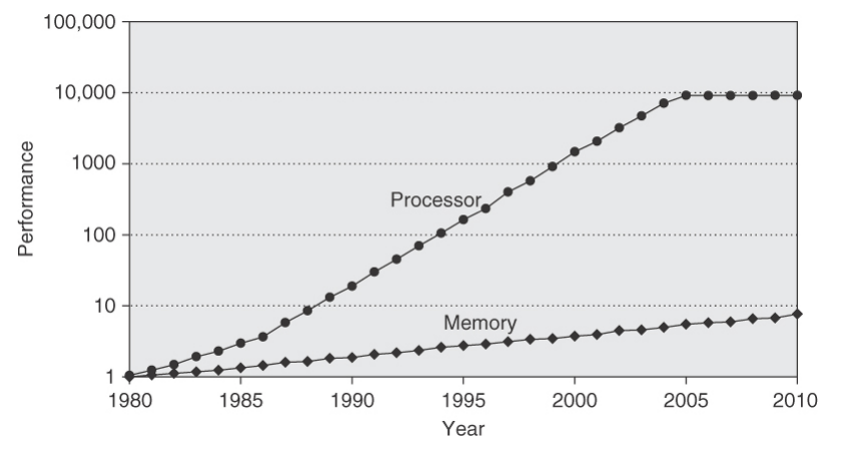
\includegraphics[width=0.7\linewidth]{fig/cpuvsmemory.jpg}
\caption{\it{The gap in performance, measured as the difference in the time 
between processor memory requests (for a single processor or core) and the 
latency of a DRAM access, is plotted over a $30$ year span~\cite{comparchbook}.}}
\label{fig:cpuvsmemory}
\end{figure}
%---------------------------
In multi-core systems, shared memory access conflicts between cores result in large access request queues. Figure~\ref{fig:multicore_arch}  illustrates a general multi-core architecture. The bank queues are served every memory clock cycle and the acknowledgement with data is sent back to the corresponding processor. In scenarios where multiple cores request access to memory locations in the same bank, the memory controller arbitrates them using bank queues. This contention between cores to access from the same bank is known as a {\em bank conflict}. As the number of bank conflicts increases, the resultant increases in memory access latency causes the multi-core system to slow.

%---------------------------
\begin{figure}[t!]
\centering
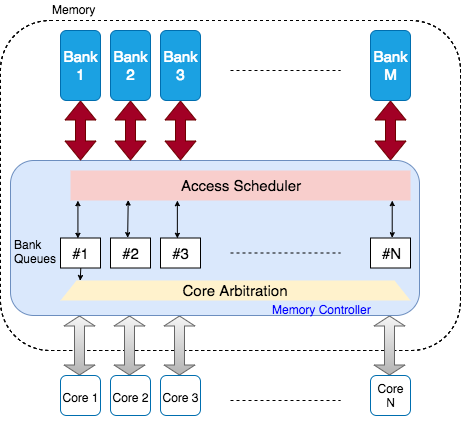
\includegraphics[width=\linewidth]{fig/fig-2-memory-controller.png}
\caption{\it{General multi-core architecture with a shared memory. $N$ processor cores share a memory consisting of $M$ banks.}}
\label{fig:multicore_arch}
\end{figure}
%---------------------------
We address the issue of increased latency by introducing a coded memory design. The main principle behind our memory design is to distribute accesses intended for a particular bank across multiple banks. We redundantly store encoded data, and we decode memory for highly requested memory banks using idle memory banks. This approach allows us to simultaneously serve multiple read requests intended for a particular bank. Figure~\ref{fig:example_xor} shows this with an example. Here, Bank 3 is redundant as its content is a function of the content stored on Banks 1 and 2. Such redundant banks are also referred to as {\em parity banks}. Assume that the information is arranged in $L$ rows in two first two banks, represented by $[a(1),\ldots, a(L)]$ and $[b(1),\ldots, b(L)]$, respectively. Let $+$ denote the XOR operation, and additionally assume that the memory controller is capable of performing simple decoding operations, \textit{i.e.} recovering $a(j)$ from $b(j)$ and $a(j) + b(j)$. Because the third bank stores $L$ rows containing $[a(1) + b(1),\ldots, a(L) + b(L)]$, this design allows us to simultaneously serve any two read requests in a single memory clock cycle.   

%---------------------------
\begin{figure}[t!]
\centering
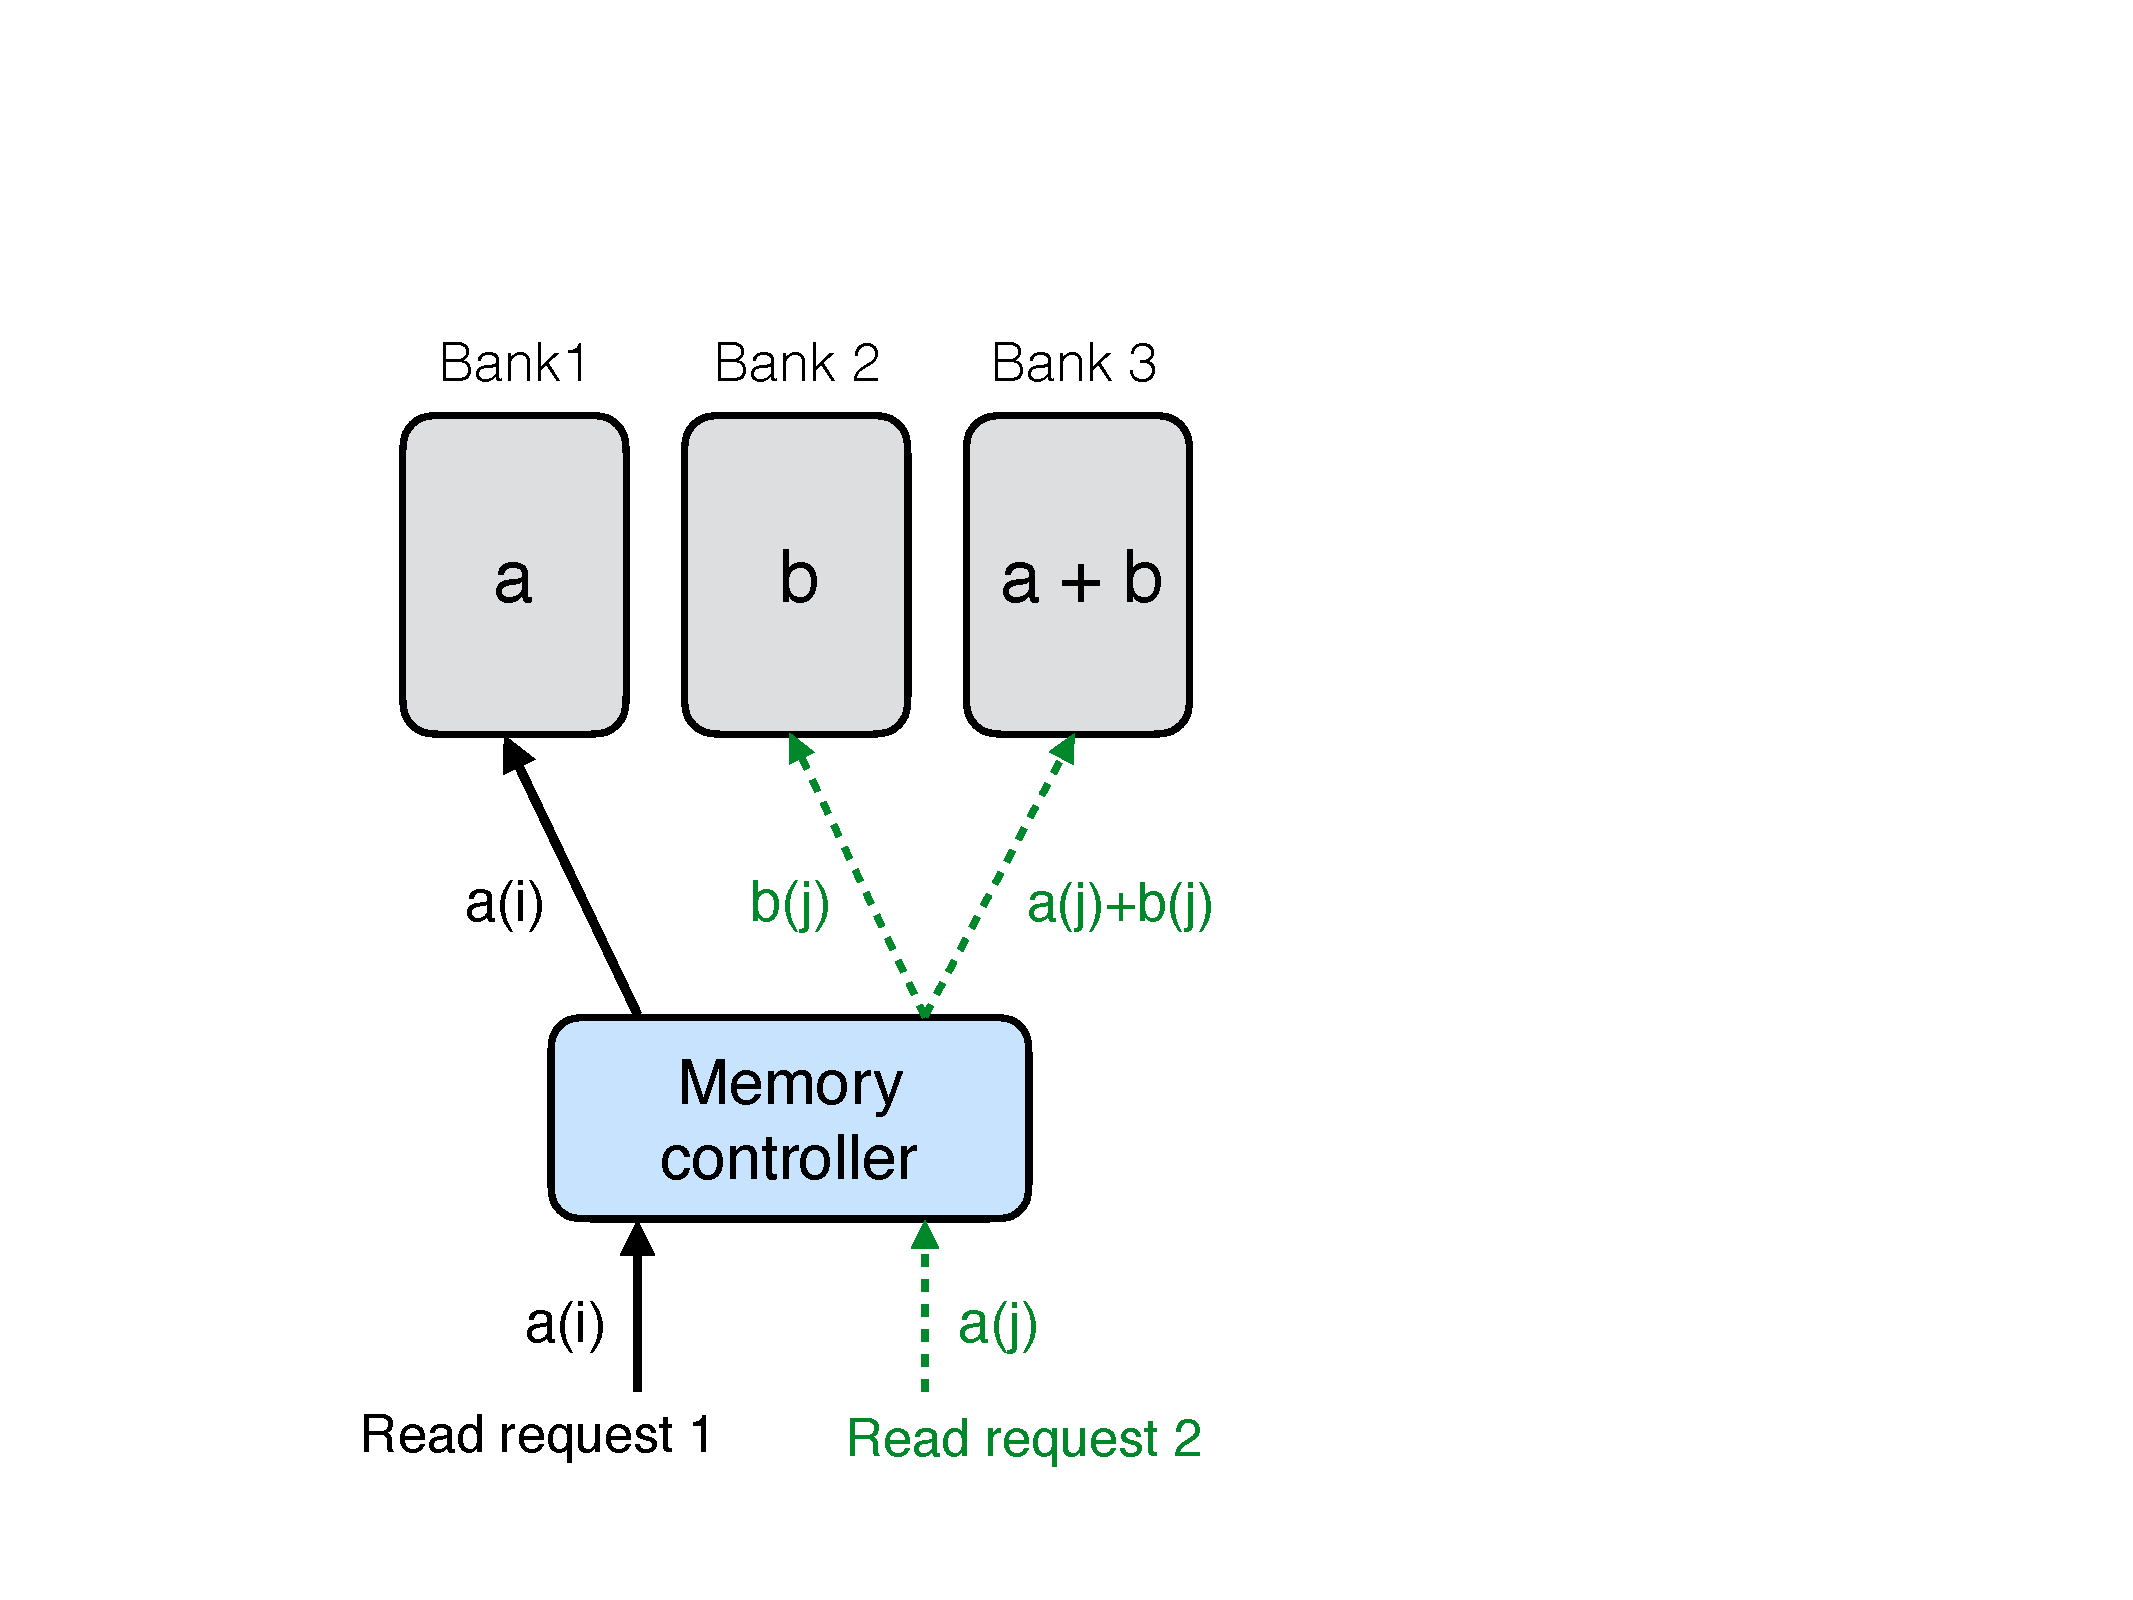
\includegraphics[width=0.395\linewidth]{fig/example-xor.pdf}
\caption{\it{Here the redundant memory in Bank 3 enables multiple read accesses to Bank 1 or 2. Given two read requests $\{a(i), a(j)\}$ directed to Bank $1$, we can deal with bank conflict in the following manner: 1) The first request for $a(i)$ is directly served by Bank $1$ itself.  2) The read request for $a(j)$ is served by downloading $b(j)$ and $a(j) + b(j)$ from Bank 2 and Bank 3, respectively. Another case where two read requests corresponding to two different banks, e.g., $\{a(i), b(j)\}$, can be simultaneously served from their respective banks without utilizing Bank $3$.}}
\label{fig:example_xor}
\end{figure}
%---------------------------
Hybrid memory designs such as the one in Figure~\ref{fig:example_xor} have additional requirements on top of serving read requests. The presence of redundant parity banks raises a number of challenges while serving write requests. The memory overhead of redundant memory storage adds to the overall cost of such systems, so efforts must be made to minimize this overhead. Finally, the heavy memory access request rate possible in multi-core scenarios necessitates sophisticated scheduling strategies to be performed by the memory controller. In this paper we address these design challenges and evaluate potential solutions in a simulated memory environment. 

\noindent \textbf{Main contributions and organization:~}In this paper we systematically address all key issues pertaining to a shared memory system that can simultaneously service multiple access requests in a multi-core setup. We present all the necessary background on realization of multi-port memories using single-port memory banks along with an account of relevant prior work in Section~\ref{sec:bg}. We then present the main contributions of the paper which we summarize below. %Here, we highlight the main contributions of the paper.
\begin{itemize}
\item We focus on the design of the storage space in Section~\ref{sec:code_design}. In particular, we employ three specific coding schemes to redundantly store the information in memory banks. These coding schemes, which are based on the literature on distributed storage systems~\cite{dimakis, Gopalan12, batchcodes, RPDV16}, allow us to realize the functionality of multi-port memories from single port memories while efficiently utilizing the storage space. Moreover, these coding schemes have low complexity encoding and decoding processes that require only simple XOR operations. %We focus on two specific memory designs that store information in memory banks based on two different coding schemes from the literature on distributed storage systems (a.k.a. cloud storage systems)~\cite{dimakis, Gopalan12, batchcodes, RPDV16}. These coding schemes allow us to realize the functionality of multi-port memories from a single port memories while efficiently utilizing the storage space. Moreover, these coding schemes have low complexity encoding and decoding processes that require only simple XOR operation.
\item We present a memory controller architecture for the proposed coding based memory system in Section~\ref{sec:memcontrol}. Among other issues, the memory controller design involves devising scheduling schemes for both read and write requests. This includes careful utilization of the redundancy present in the memory banks while maintaining the validity of information stored in them.
%In our setup, these scheduling schemes need to take the underlying coding scheme into account in order to utilize the redundancy present in the array of memory banks in the best possible manner. Furthermore, we also address the issue of keeping track of the validity of the information stored in various banks. Note that, due to unserved previous write requests, some of the stored data might have become outdate as far as a particular read request is concerned.
%able to serve the masecond main component of a shared memory system, i.e., memory controller, in Section~\ref{sec:memcontrol}. The memory controller design We also design the memory controllers for the proposed memory systems based on the storage pattern in different memory banks. Note that the memory controller design involves devising buffering and arbitration (scheduling) schemes for both read and write requests.
\item Focusing on applications where memory traces might exhibit favorable access patterns, we explore two ways to improve the efficiency of our coding based memory design in Sections~\ref{sec:dynamicCoding} and~\ref{sec:prefetching}. First, we propose a dynamic coding scheme which is based on detection of continuous heavily accessed regions of memory. 
%The dynamic coding scheme only encode these heavily access regions at a particular time instance. As different (uncoded) regions begin receiving more accesses, the dynamic coding scheme updates the content of parity (redundant) memory banks by encoding these regions. 
The second solution involves predicting the patterns of memory addresses over time. 
%Based on this prediction, the data from free bank is prefetched to serve subsequent request for information with the help of the prefetched data. This creates the opportunities to serve a large number of access requests in a given memory clock cycle. We note that the design of such prefacing schemes crucially depends on the underlying coding scheme.
%with Accompanied the design using dynamic coding where data is moved between coded and uncoded states. Utilized the coded memory system to perform useful data prefetching.
\item Finally, we conduct a detailed evaluation of the proposed designs of shared memory systems in Section~\ref{sec:experimentalmethodology}. We implement our memory designs by extending Ramulator, a DRAM simulator.~\cite{Ramulator}. We use the gem5 simulator~\cite{parsec_2_1_m5} to create memory traces of the PARSEC benchmarks~\cite{bienia09parsec2} which are input to our extended version of Ramulator. We then observe the execution-time speedups our memory designs yield.%a Implementation of the proposed solution using system C. Performance evaluation of the proposed solution on real memory traces with the help the system C implementation.  evaluate each
%of them for their cost. We also implement these designs using systemC and regress it throughmemory traces from real multi-core system.
\end{itemize}

%problem of concentrated accesses to a particular bank by normalizing it across 
%several banks. The solution is to use coding theory techniques to create 
%redundancy across banks, increasing the number of parallel accesses per cycle.  
%The queue build up on a bank is serviced through parallel access to several 
%additional banks, known as parity banks. The additional bank accesses results in 
%a decrease in number of contended memory accesses between cores, therefore 
%reducing the overall latency of the system. The reduction in the latency can be 
%seen directly as an increase in the overall system performance. 
%We present various design to store the redundancy across the parity banks and evaluate each
%of them for their cost. We also implement these designs using systemC and regress it through
%memory traces from real multi-core system.
%We show that 
%with a memory overhead of 15 $\%$; we can enable 4 extra read accesses / 2 extra 
%write accesses to a bank while remaining within the given design parameters. 

%{\color{blue}
%\subsection{Main contributions}
%
%Here, we summarize the main contributions of this paper. 
%\begin{itemize}
%\item Taking a coding theoretic approach to address the issue of realizing multi-port memories from single port memories. 
%\item Designed the memory controller accordingly:
%\begin{itemize}
%\item Involves devising scheduling schemes for both read and write requests.
%\end{itemize}
%\item Accompanied the design using dynamic coding where data is moved between coded and uncoded states. 
%\item Utilized the coded memory system to perform useful data prefetching.
%\item Implementation of the proposed solution using system C. Performance evaluation of the proposed solution on real memory traces with the help the system C implementation. 
%\end{itemize}
%}

%\noindent \textbf{Organization:~} The rest of the paper is organized as follows.

%\textbf{Key issues that need to be addressed}

%\begin{itemize}
%\item Design of storage space, i.e., how the data is distributed among different memory banks. This includes generation of redundancy (parity bits) based on the original data and allocation of these parity bits to the memory banks.
%\item Keeping track of the validity of the data stored in various banks. Note that, due to unserved previous write requests, some of the stored data might have become outdate as far as a particular read request is concerned.
%\item Resource allocation/arbitration among the different read and write requests originated from the same or different processors. The arbitration mechanism should take multiple criterion into account, including performance (i.e., the latency viewed by the processors), efficient utilization of the storage space (i.e., minimize the unused memory bank during a given period of time), and fairness (i.e., no processor should unnecessarily suffer due to requests from other processors getting prioritized).
%\end{itemize}

%%%%%%%%%%%%

%%%%%%%%%%%%%%%%%%%%%%%%%%%%%%%%%%%%%%%%%%%%%%%%%%%%%%%%
% Background and Related Work
%%%%%%%%%%%%%%%%%%%%%%%%%%%%%%%%%%%%%%%%%%%%
\section{Background and Related Work}
%\section{Preliminaries and Related Work}
\label{sec:bg}

\subsection{Emulating multi-port memories}
\label{sec:emulation}

The multi-port memories are essential to provide seamless memory accesses in a multi-core setup as these memories can support simultaneous accesses to data elements (which are potentially stored on the same memory bank) by multiple cores. However, designing a true multi-port comes at a large cost. Besides complex circuit implementation for I/O, the area requirements for multi-port bit-cells is significantly higher than that for single-port bit-cells~\cite{Suzuki,WLCH14}. This motivates the exploration of algorithmic and system level designs to emulate multi-port memories using simple and area efficient single-ported memory banks~\cite{ACP88, EMY91, RG91,Memoir_xor, Memoir_xor_virtual}. Attempts have been made to emulate multi-port memory by \cite{CCES93}, however they use replication based design that makes the resulting architecture very large in memory. \Ethan{Move some of this earlier?}

%\Ankit{This patent by  Chappell, Chappell, Ebcioglu and Schuster\cite{CCES93} arguing against both multi-port RAMs and their emulation using single-port RAMs. But the emulation is replication based so we can make a case here for coding based emulation.....}

Due to space limitations we focus on specific, illustrative request patterns. We invite the reader to verify that our designs indeed handle the set of all possible requests.

\subsubsection{Read-only Support} 
\label{sec:read_only}
Replication-based designs are the most prevalent candidates in this design space. Assuming that a memory design is required to support only read requests, say $r$ read requests per memory clock cycle, one can simply store $r$ copies of each data element on $r$ different single-port memory banks. In every memory clock cycle, the $r$ read requests can be served in a straightforward manner by mapping all read request to distinct memory banks (see Figure~\ref{fig:read_replication}). This way, the $r$-replication-based design completely avoids bank conflicts for up to $r$ read request in a memory clock cycle. 

\begin{remark}
\label{rem:read_only}
If we compare the memory design in Figure~\ref{fig:read_replication} with that of Figure~\ref{fig:example_xor}, we notice that both designs can simultaneously serve $2$ read requests without causing any bank conflicts. Note that the design in Figure~\ref{fig:example_xor} consumes smaller storage space as it needs only $3$ single-port memory banks while the design in  Figure~\ref{fig:read_replication} requires $4$ single-port memory banks. However, for the design in Figure~\ref{fig:example_xor}, the access process involves some computation. {\color{red}This observation indeed generalizes to the conclusion that the sophisticated coding schemes allow for better storage efficient designs as compare to the replication based design~\cite{MacSlo}. However, this comes at the expense of increased computation (XOR decoding). Therefore, it is important to employ those coding schemes that enable storage efficiency with as small computational overhead as possible.}
\end{remark}

%---------------------------
\begin{figure}[t!]
\centering
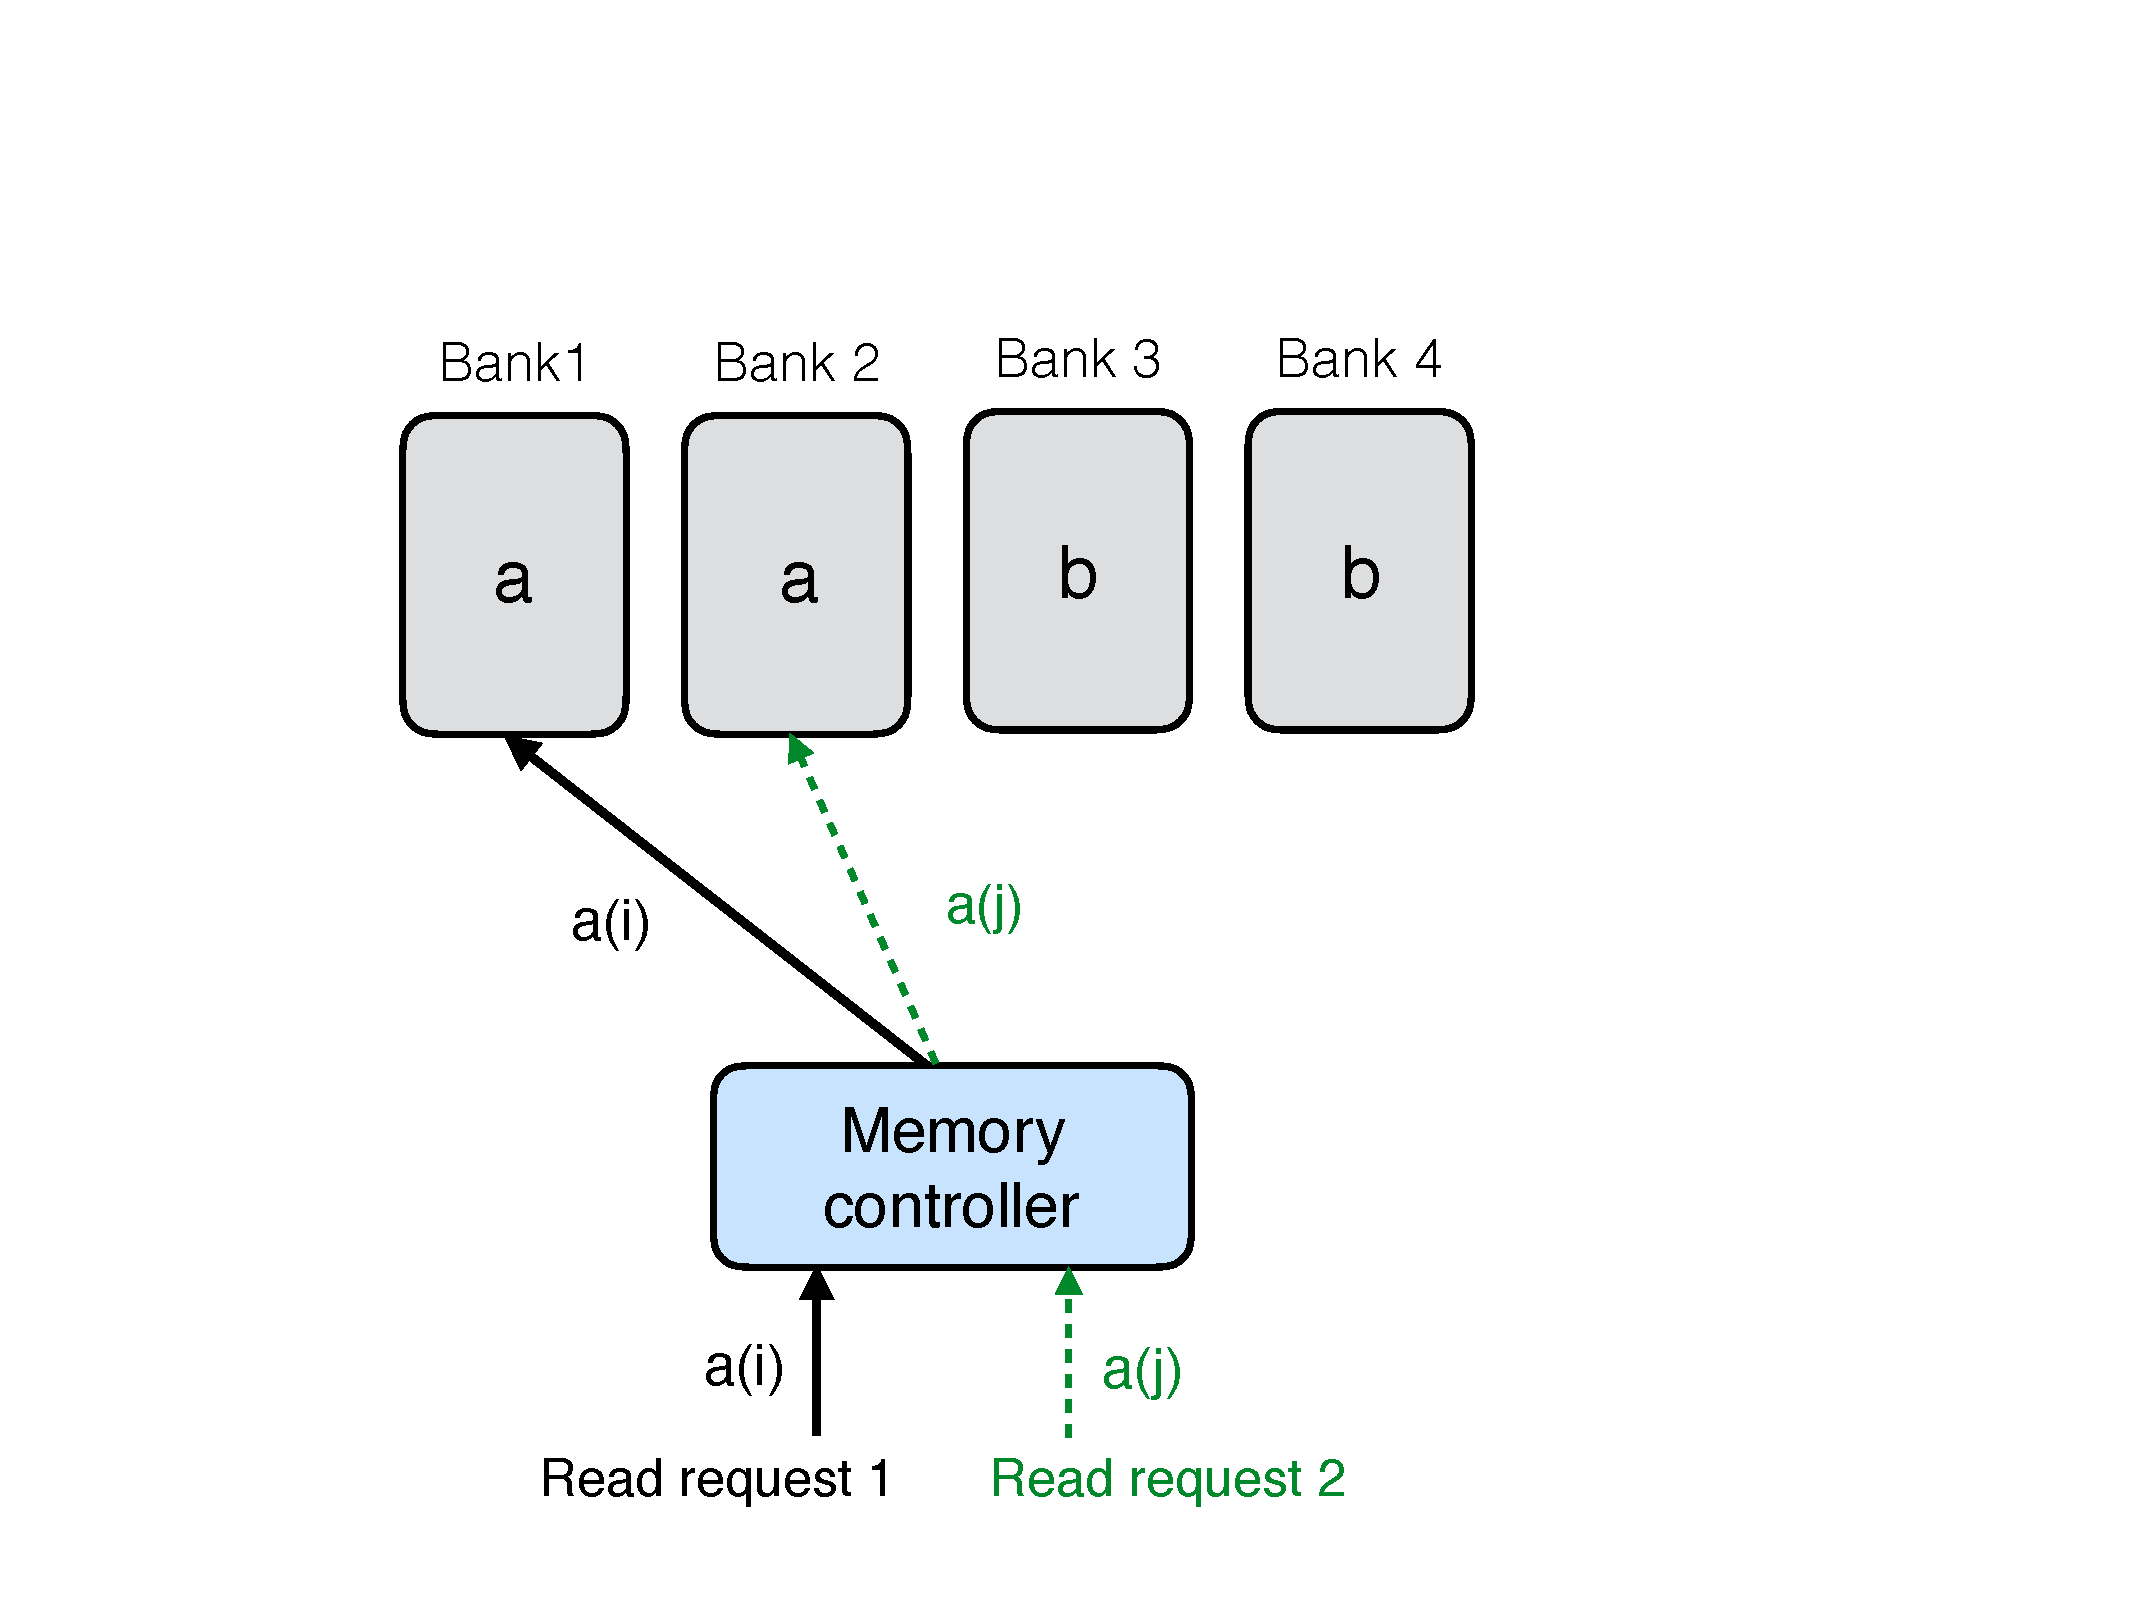
\includegraphics[width=0.425\linewidth]{fig/read-replication.pdf}
\caption{$2$-replication based design to support multiple $2$ read requests in the same memory clock cycle. The two banks' worth of data $\mathbf{a} = [a(1),\ldots, a(L)]$ and $\mathbf{b} = [b(1),\ldots, b(L)]$, all the data elements are stored on two distinct memory banks. Note that any $2$ read requests to distinct memory banks. For example, the figure considers the scenario with $2$ read requests for elements $\{a(i), a(j)\}$. Since both $a(i)$ and $a(j)$ are stored on $2$ banks, one of those banks can be used to serve each request without causing any bank conflicts. It's straightforward to verify that this memory design avoids bank conflicts for any other set of $2$ read requests.}
\label{fig:read_replication}
\end{figure}
%---------------------------

%---------------------------
\begin{figure}[t!]
\centering
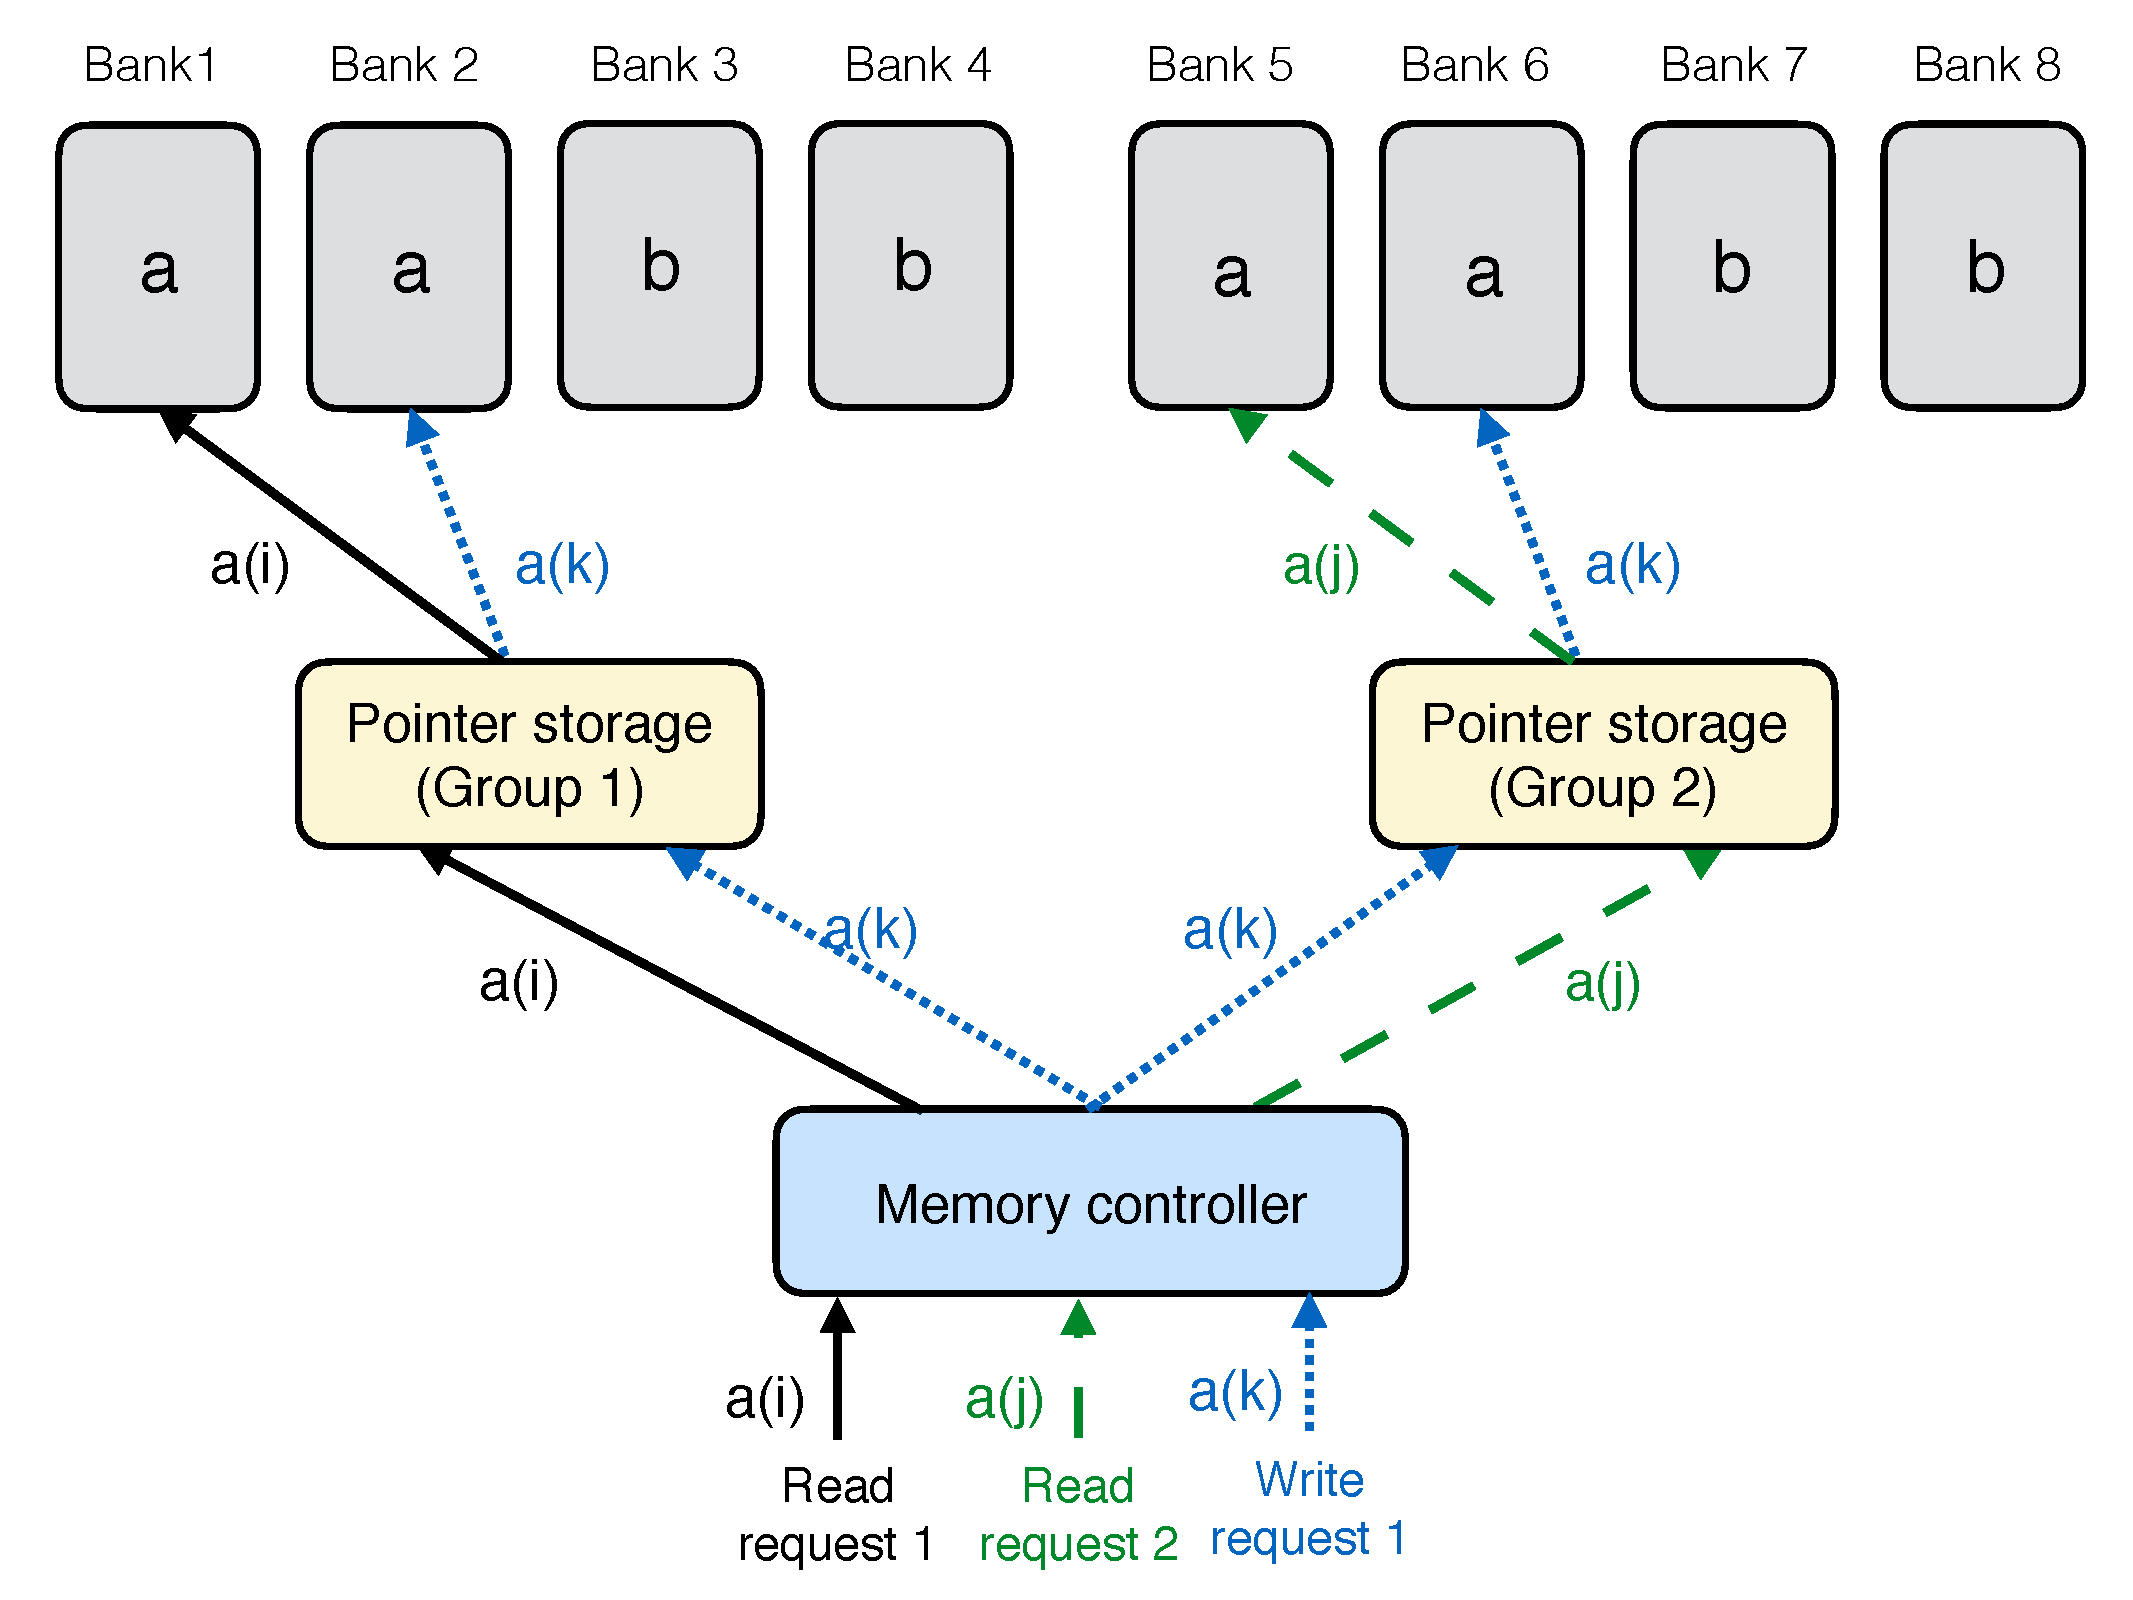
\includegraphics[width=0.86\linewidth]{fig/rw-replication.pdf}
\caption{$4$-replication based design to support $r = 2$ read requests and $w = 1$ write request in one memory clock cycle. Both collections of information elements $\mathbf{a} = [a(1),\ldots, a(L)]$ and $\mathbf{b} = [b(1),\ldots, b(L)]$ are replicated on $r\cdot (w + 1) = 4$ different single-port memory banks. These banks are then partitioned into $r = 2$ disjoint groups. We utilize each group to serve one read request. In a given memory clock cycle, we focus on the specific access pattern with the read requests for $\{a(i), a(j)\}$ and the write request for $\{a(k)\}$. Assuming that Bank $1$ (from Group $1$) and Bank $5$ (from Group $2$) have the updated versions of the data elements $a(i)$ and $a(j)$, respectively, we serve the read requests for $a(i)$ and $a(j)$ from Bank $1$ and Bank $5$, respectively. As for the write request for the data element $a(k)$, we need to perform this write request in at least one memory bank in each of the two groups. This will enable both groups to continue serving any possible set of $r = 2$ read requests during future accesses. Since we have one memory bank storing $a(k)$ in each of the groups that is not busy serving write request, we write the updated $a(k)$ in these non-busy banks (Bank $2$ and Bank $3$ in this case). During the writing process, we also need to modify the pointer storage accordingly to keep track of the banks in each group that are storing the most updated values of different data elements.}
\label{fig:rw_replication}
\end{figure}
%---------------------------
\subsubsection{Read and Write Support}
\label{sec:rw}
\Ankit{Mainly describing the results from the work of Auerbach, Chen, and  Paul\cite{ACP88}.} 
% It is evident from the discussion so far that we can indeed emulate the behavior of a multi-port memory on read requests by storing data on single-port memory banks in a redundant manner. 
The redundancy mechanism can vary from simple replication-based strategy to more sophisticated coding schemes. However, a successful memory design necessarily need to address the issues of (potentially multiple) write requests as well. A challenge that arises in the presence of write requests is that one also need to ensure consistency across different requests. This requires managing multiple versions of the same information across all the memory banks and making sure that stale information is not supplied in response to a particular read request. 

Restricting ourselves to replication-based designs, a multi-port memory that simultaneously supports $r$ read requests and $w$ write requests in a memory cycle can be emulated by  using a $r\cdot(w + 1)$ replication scheme, where $r\cdot(w+1)$ copies of each data element are stored on $r\cdot(w + 1)$ different single-port memory banks. We illustrate this scheme for $r = 2$ and $w = 1$ in Figure~\ref{fig:rw_replication}. According to all of our previous illustrations, we assume that we have two symbols' worth of information $\mathbf{a} = [a(1),\ldots, a(L)]$ and $\mathbf{b}  = [b(1),\ldots, b(L)]$. We store $4$ copies each of data elements $\mathbf{a}$ and $\mathbf{b}$ and partition the banks that store a data element into $r = 2$ disjoint groups with each group containing $(w + 1) = 2$ memory banks. In Figure~\ref{fig:rw_replication}, Banks $1$ -- $4$ and Banks $5$ -- $8$ correspond to Group $1$ and Group $2$, respectively. For the underlying replication-based scheme, we also require additional storage space to keep track of the versions of different copies of the information elements. This space is referred to as the pointer storage. In Figure~\ref{fig:rw_replication}, we illustrate how this design serves a particular set of $2$ read requests and $1$ write request.\\

\noindent \textbf{Additional cost to support write requests:~} Let's look at the additional cost associated with the requirement of being able to support write requests. Recall that the $r$-replication enables us to serve any set of $r$ read requests in a memory clock cycle. Demanding that we also support $w$ write requests, the required replication factor of the replication-based design jumps to $r\cdot(w + 1)$. This follows as we use $r$ different groups of banks to serve $r$ different read requests. In order to avoid bank conflicts this requires that, for every data element, there should be at least one memory bank that store the most update version of that data element at the beginning of every memory clock cycle. Thus, we should be able to perform $w$ write requests in each of the groups of memory banks. Since we have $w$ write and $1$ read operations to perform in every group, we require at least $(w + 1)$ memory banks in each of the $r$ groups. This amounts to the replication factor of $r\cdot(w +1)$. Furthermore, the memory design also requires additional storage space to keep track of the locations of the updated versions of each of the data element. This storage space is referred to as pointed storage in Figure~\ref{fig:rw_replication}. \Ethan{condense the beginning of this paragraph, and move the end of this paragraph later since it's not really background} Note that in order to ensure that the pointer storage space is small, we need to continuously update all the replicas of each data element. For data elements that do not have an entry corresponding to them in the pointer storage, we assume that all of their replicas are storing their current version. This process of synchronization across the replicas of a data element is opportunistically performed on the different banks storing the replicas when these banks are not busy serving access requests from the cores. Therefore, we have two components of the additional cost for the ability to support write requests: 1) Storage space for more replicas and pointer storage and  2) Continuous background maintenance task of synchronizing all the replicas of a data element with its current version. 

\begin{remark}
\label{rem:rw}
As illustrated above, an $r$-replication based design to serve $r$ read request can be modified to an $r\cdot(w+1)$-replication based design to support $r$ read and $w$ write requests. If we focus on memory design that supports multiple read requests by using sophisticated coding schemes (e.g., the design in Figure~\ref{fig:example_xor}), we can modify it to support both read and write requests as well. A generic approach that can be used to support $r$ read requests and $w$ write requests is as follows\footnote{We note that depending on the specific coding scheme, one can present a more storage-efficient design. Here, we present a universal scheme that works for any coding scheme.}.Take a coding scheme based memory design that can serve any set of $r$ read requests. Now replicate this whole design $(r + w)$ times. These $(r + w)$ copies of the original design are considered as $(r + w)$ different groups. Now, given $r$ read requests we look for minimum number of groups that store the most updated version of the data elements associated with these read requests and serve all the read requests. In the worst case this would require using $r$ different groups. For the $w$ write requests, we commit these $w$ requests to $w$ different groups that are not used to serve read requests. Note that there are at least $w$ such groups. While performing a write request inside a group, we update all the memory banks of the group according to the write request. Similar to the $r\cdot(w + 1)$-replication based design, this design also requires additional storage space to store pointers to keep track of the groups storing the most  updated version of the data elements. Furthermore, In order to keep this storage space small, we again need to opportunistically synchronize all the banks with the most recent version of the data elements.\Ethan{rewrite}
\end{remark}

%\subsection{Better emulation of multi-port memories}
\subsection{Storage-efficient emulation of multi-port memories}
\label{sec:efficient_emulation}

As described in Section~\ref{sec:emulation}, by utilizing various ways to introduce redundancy (ranging from simple replication to more sophisticated coding schemes) it's possible to design a memory based on only single-port memory banks that emulate the behavior of a multi-port memory. In a setup where only read requests need to be served (cf. Section~\ref{sec:read_only}) such an emulation is less costly to achieve, both in terms of storage and computational cost. In particular, by careful selection of the underlying coding scheme, it's possible to serve multiple read requests by incurring both small storage and computational overhead (cf.~Remark~\ref{rem:read_only}). \Ethan{remove?}

However, the emulation become much more costlier in the scenario when write requests also needs to be performed (cf. Section~\ref{sec:rw}). Besides the increment in the number of single-port memory banks, the ability to serve write requests also requires the installation of pointer storage to keep track of the various versions of the data elements present in the memory banks. As highlighted in Section~\ref{sec:rw}, it's necessary to continuously synchronize all the memory banks storing a particular data element in order to keep the pointer storage space small. \Ethan{remove above this line, put below this line somewhere earlier?} Furthermore, the presence of varying version in the banks also complicates the process of arbitration, \textit{i.e.} mapping access requests to memory banks, as read requests need to be served by the bank storing the current version of the data element. Since most of the programs in a multi-core would involve significant amount of write requests, any design to emulate multi-port memory using single-port memory needs to take these overheads into account. 

{\color{red}We believe that various tasks that arise in the presence of write requests and contribute to computational overhead of the memory design, including synchronization among memory banks and complicated arbitration, can be better managed at the algorithmic level.\Ethan{good point!} Note that these tasks are performed at memory controller. It's possible to reduce the effect of these tasks on the overall performance of memory system by relying on the increasing available computational resources while designing the memory controller. On the other hand, we believe that the storage overhead is a more fundamental issue that needs to be addressed for the emulation of the multi-port memories to be viable and appealing. In particular, the large replication factor in a naive design (cf.~Remark~\ref{rem:rw}) limits the applicability of the obtained memory in practice due to large storage overhead and the associated large area requirement resulting from this.}

In order to reduce the storage overhead, we avoid the two step (naive) memory design process highlighted in Remark~\ref{rem:rw}: 1) First, employ a coding scheme that can serve multiple read requests, and 2) Then replicate the obtained memory bank arrangement multiple times in order to support write requests as well. We instead encode the data elements using specific coding schemes which create parity banks by encoding over a multiple data banks and have reasonably high rate. We select the underlying coding scheme to support multiple read requests in the worst case. Instead of replicating the obtained design, we exploit the fact we do not always encounter worst case pattern for read request and the obtained design can potentially serve access patterns with much larger number of read requests. In other words, for many access patterns with a given number of read requests, there are many memory banks that remain unused. These unused banks are generally available to perform (part of) pending write requests. Therefore, if one aims at performing arbitration among access requests arising over a slightly longer duration as opposed to focusing on requests arriving at each memory clock cycle, all the requests can be served without\Ethan{with? also rewrite this paragraph} good latency. In this way, instead of designing various components of the memory system, e.g., bank array and memory controller, independently, taking the holistic view of the entire memory system allows us to not commit unnecessary storage space in terms of large number of bank which only provide small amount of utility in terms of performance of the system. We recognize that this approach leads to increased complexity at the memory controller. {\color{red} {\em However, we show that the increment in the complexity can be kept within the acceptable level while insuring storage-efficient emulation of multi-port memories with the help of better algorithmic design.}}

\subsection{Related work}

Coding theory is one of the well studied field which deals with mitigating the adversarial effects of the underlying medium in an information processing system~\cite{MacSlo, Cover}. In particular, the developments in the field have enabled both reliable communication across noisy channel and storage over fault-prone storage units in resource efficient manners. Recently, we have witnessed intensive efforts towards the applications of coding theoretic ideas to design large scale distributed storage systems~(see e.g., \cite{Azure, SAPDVCB13, Rashmi14}). In this domain of coding for distributed storage systems, the issue of access efficiency has also received attention, especially the ability to support multiple simultaneous read accesses with small storage overhead~\cite{batchcodes, RPDV16, RSDG16, Wang2017} and references therein. In this paper, we rely on the coding techniques developed under in this domain to realize emulation of multi-port memories using single-port memory banks. However, we note that the existing work on batch codes~\cite{batchcodes} only focuses on the read requests. On the other hand, the successful emulation of multi-port memory also requires handling write requests in an efficient manner. Furthermore, the design presented in this paper also needs to address the entire memory system which also involves memory controller design as opposed to just focusing on the storage array. 


Here, we note that the issue of designing coding schemes that have low update complexity, \textit{i.e.} that can be modified with low overhead as the information gets updated, have also received some attention in the literature (see e.g.,~\cite{ASV10, MCW14}). However, this treatment is extensive enough to address the update issues that arise in the context of our memory systems, where write requests may be very frequent and a large portion of the bank array needs to get updated. Again, the key issue that distinguish our work from the majority of the literature on coding for distributed storage is that we need to take the interplay among read and write requests and its effect on the overall performance (latency) into account.\Ethan{good point} Furthermore, we  are not allowed to encode across a very large number of storage units (memory banks in our case), which is very much feasible in today's large scale cloud storage systems.

In this paper, we also explore the idea of proactively prefetching the information from memory banks to improve the access efficiency of our memory design. The idea of prefetching in realizing fast data transfer between processors and memory has been previously explored in the literature (see \cite{Kim2016, Kadjo2014, Shevgoor2015, JL2013} and references therein). 
%However, our work addresses the issue of data prefetching in the context of coded memory system which is not addressed earlier in the literature. 
More recently, an LSTM-based recurrent neural network was used to predict future memory access requests on the SPEC 2006 benchmark dataset \cite{lstm2018}. This deep learning method may be used in addition to our proposed frequency-based approach.
Our combination of coded memory and prefetching also shares some similarity with the recent line of work on coded caching~\cite{MN16a} which aims to reduce the data downloaded from servers in a communication network by utilizing the cache available at the end users. Here, we would like to point out that there are many key differences in the our setup with coded memory banks with that considered in \cite{MN16a}. Our setup has data stored in an encoded form stored across memory banks and caching is enabled by the memory controller, which is a centralized unit. In contrast, the setup of coded caching has a centralized storage system (server) and cache units that store encoded information distributed across users.

{\color{red} {\bf The work which is closest to our solution for emulating a multi-port memory is by Iyer and Chuang~\cite{Memoir_xor, Memoir_xor_virtual}, where they also employ XORing based coding schemes to redundantly store information in an array of single-port memory banks. However, we note that our work significantly differers from \cite{Memoir_xor, Memoir_xor_virtual} as we specifically rely on different coding schemes arising under the framework of batch codes~\cite{batchcodes}. Additionally, due to the employment of distinct coding techniques, the design of memory controller in our work also differs from that in \cite{Memoir_xor, Memoir_xor_virtual}.}}

\Ankit{Also cite the work by Rivest et al.~\cite{RG91} and Endo, Matsumura and Yamada~\cite{EMY91}.}

%\section{Motivation}
%
%\subsection{Dual port RAM}
%
%\subsubsection{Replication}
%Because the size of the dual-ported SRAM bit-cell is almost double that of the single-ported SRAM bit-cell, a more versatile way (i.e., can do 2 reads in one cycle or one write) to implement dual-ported SRAM is by duplicating SRAM banks, as shown in Figure 3. In this way the bandwidth does not suffer from any loss for performing 2 simultaneous read operations, but only suffers 1 arbitration loss when performing simultaneous read and write operations (i.e., cannot perform 1 read and 1 write in the same cycle). The area is similar to that used in dual-ported circuit implementations. The advantage of this implementation is simplicity while the disadvantage is that if frequent write access is required the performance (bandwidth) is not as good as the true 1R1W SRAMs which can do a simultaneous read and write in one cycle.
%
%\subsubsection{Replication with pointer storage}
%
%Replication scheme $r + w$ replications...for $rRwW$ multipart memory.
%
%\subsubsection{Bank interleaving and arbitration}
%
%Another alternative is to use bank interleaving and arbitration circuits to allow for simultaneous access of different banks of memory. Occasional stalls are necessary in this approach if the arbitration circuit finds conflicting access to the same memory banks. Its operation is illustrated in Figure 4.
%
%Figure 4. Multiple accesses to SRAM by Bank interleaving with lower address bits. A large SRAM bank is sub-divided into n (n ? 2) smaller single-ported SRAM banks to support 2 or more simultaneous accesses. An arbitration unit is used in case conflicting addresses want to access the same bank, in which case one of the accesses is delayed.
%
%
%
%
%{\color{red}
%SRAMs can be categorized as single-ported or multi-ported. The single-ported SRAM is the most common type of SRAM with the best area efficiency and is used for most compiler memories due to its modular approach. Multi-ported memories are either not area efficient or with limited storage capability. Logical implementation of multi-ported memories with interleaved banks can be area efficient (because there is no memory duplication), but requires arbitration and flow-control circuits. Duplicating single-ported memory banks can support 2 reads and 1 write type of accesses with no additional delays and 1 read and 1 write type of access with 1.5 times the delay of read access;  Also its size is competitive relative to the true dual-ported memories. True multi-ported memories can be implemented with single-ported memories by replicating the memories multiple times. The area cost is r(w+1) times the number of bank replications.  Algorithmic approaches of multi-port memory design (such as Memoir) include caches and different ways of buffering of read and write data, with advantages being area efficiency and disadvantages including design complexity. Algorithmic memories can be statistical with lower areas or deterministic with higher areas, depending on the application.}



%%%%%%%%%%%%%%%%%%%%%%%%%%%%%%%%%%%%%%%%%%%%%%%%%%%%%%%%
% Code design
%%%%%%%%%%%%%%%%%%%%%%%%%%%%%%%%%%%%%%%%%%%%
\section{Codes to Improve Accesses}
\label{sec:code_design}

%In this section, we discuss one of the main components of the memory design proposed in this paper. 
Introducing redundancy into a storage space comprised of single-port memory banks enables simultaneous memory access. In this section we propose memory designs that utilize coding schemes which are designed for access-efficiency. We first define some basic concepts with an illustrative example and then describe $3$ coding schemes in detail.

\begin{comment}
Coding theory is the study of codes and their applications  to specific fields.  
Coding has been used in a variety of computer  science applications,  from error 
correction in the transmission of data  to increased compression for data  
storage.  We aim to extend the benefits of coding theory  to improve the 
efficiency of random-access  memory systems.  We propose a memory scheme in 
which a small portion of memory is reserved for the efficient coding of 
pre-existing data.  In essence, this allows the data of one bank to be 
duplicated and stored in an additional memory location.  Traditionally, when 
multiple  requests  to a single bank  are issued by the processor, a stall is 
generated.  These types of stalls, known as bank conflicts, result from the fact 
that  only one address from a single bank can be accessed at a time.  The 
processor must wait for the result from the first bank access to return  before 
it can serve additional  requests to the same bank.  This lag can be a major 
bottleneck in a computer's processing speed. With a coded memory scheme, data 
present in multiple data banks will be compressed and stored in extra banks, 
known as a parity banks.  These parity banks will then be accessed concurrently 
with corresponding data  banks to help alleviate stalls from bank conflicts.  
Ultimately,  with the addition  of a single parity  bank we are able to generate 
a single additional  access to any arbitrary bank  without  implementing  any 
further  logic to the bank  itself.  In the following sections, we first 
describe the design parameters used to design the coding system.  We then 
describe each of the three code schemes explored in this project.
\end{comment}

\subsection{Coding for memory banks}
\label{sec:coding_mb}

A coding scheme defines how memory is encoded to yield redundant storage. The memory structures which store the original memory elements are known as {\em data banks}. The elements of the data banks go through an {\em encoding process} which generates a number of {\em parity banks}.  The parity banks contain elements constructed from elements drawn from two or more data banks. A linear encoding process such as XOR may be used to minimize computational complexity. The following example further clarifies these concepts and provides some necessary notation.

\begin{example}
Consider a setup with two data banks $\mathbf{a}$ and $\mathbf{b}$. We assume that each of the banks store $L \cdot W$ binary data elements\footnote{It is possible to work with data elements over larger alphabets/finite fields. However, assuming data elements to be binary suffices for this paper as only work with coding schemes defined over binary field.} which are arranged in an $L \times W$ array. In particular, for $i \in [L] \triangleq \{1,\ldots, L\}$, $a(i)$ and $b(i)$ denote the $i$-th row of the bank $\mathbf{a}$ and bank $\mathbf{b}$, respectively. Moreover, for $i \in [L]$ and $j \in [W] \triangleq \{1,\ldots, W\}$, we use $a_{i, j}$ and $b_{i, j}$ to denote the $j$-th element in the rows $a(i)$ and $b(i)$, respectively. Therefore, for $i \in [L]$, we have 
\begin{align}
a(i) = \big(a_{i,1}, a_{i,2},\ldots, a_{i, W}\big) \in \{0, 1\}^W\nonumber \\
b(i) = \big(b_{i,1}, b_{i,2},\ldots, b_{i, W}\big) \in \{0, 1\}^W. \nonumber
\end{align}
Now, consider a linear coding scheme that produces a parity bank $\mathbf{p}$ with $L'W$ bits arranged in an $L' \times W$ array such that for $i \in [L'] \triangleq \{1,\ldots, L'\}$, 
\begin{align}
p(i) &= \big(p_{i, 1},\ldots, p_{i,W}\big) = a(i) + b(i) \nonumber \\
&\triangleq \left(a_{i,1} + b_{i,1}, a_{i,1} + b_{i,1},\ldots, a_{i,1} + b_{i,1}\right). 
\end{align}
\end{example}
\begin{remark}
Figure~\ref{fig:example1} illustrates this coding scheme. Because the parity bank is based on those rows of the data banks that are indexed by the set $[L'] \subseteq [L]$, we use the following concise notation to represent the encoding of the parity bank. 
$$
\mathbf{p} = \mathbf{a}([L']) +  \mathbf{b}([L']).
$$
In general, we can use any subset $\mathcal{S} = \{i_1, i_2,\ldots, i_{L'}\} \subseteq [L]$ comprising $L'$ rows of data banks to generate the parity bank $\mathbf{p}$. In this case, we have $\mathbf{p} = \mathbf{a}(\mathcal{S}) +  \mathbf{b}(\mathcal{S})$, or
\begin{align*}
p(l) = a(i_l) + b(i_l)~\text{for}~l \in [L'].
\end{align*}
%Figure~\ref{fig:example1_case2} illustrates the case with a generic set $\mathcal{S}$.% $ = [L - L'  + 1,\ldots, L]$.
\end{remark}

%%%%%%%%%%%%%%%%%%%%%%%%%%%%%%%%%%%
%\begin{figure}[t!]
%\centering
%\begin{subfigure}[b]{0.48\linewidth}
%  \centering
%  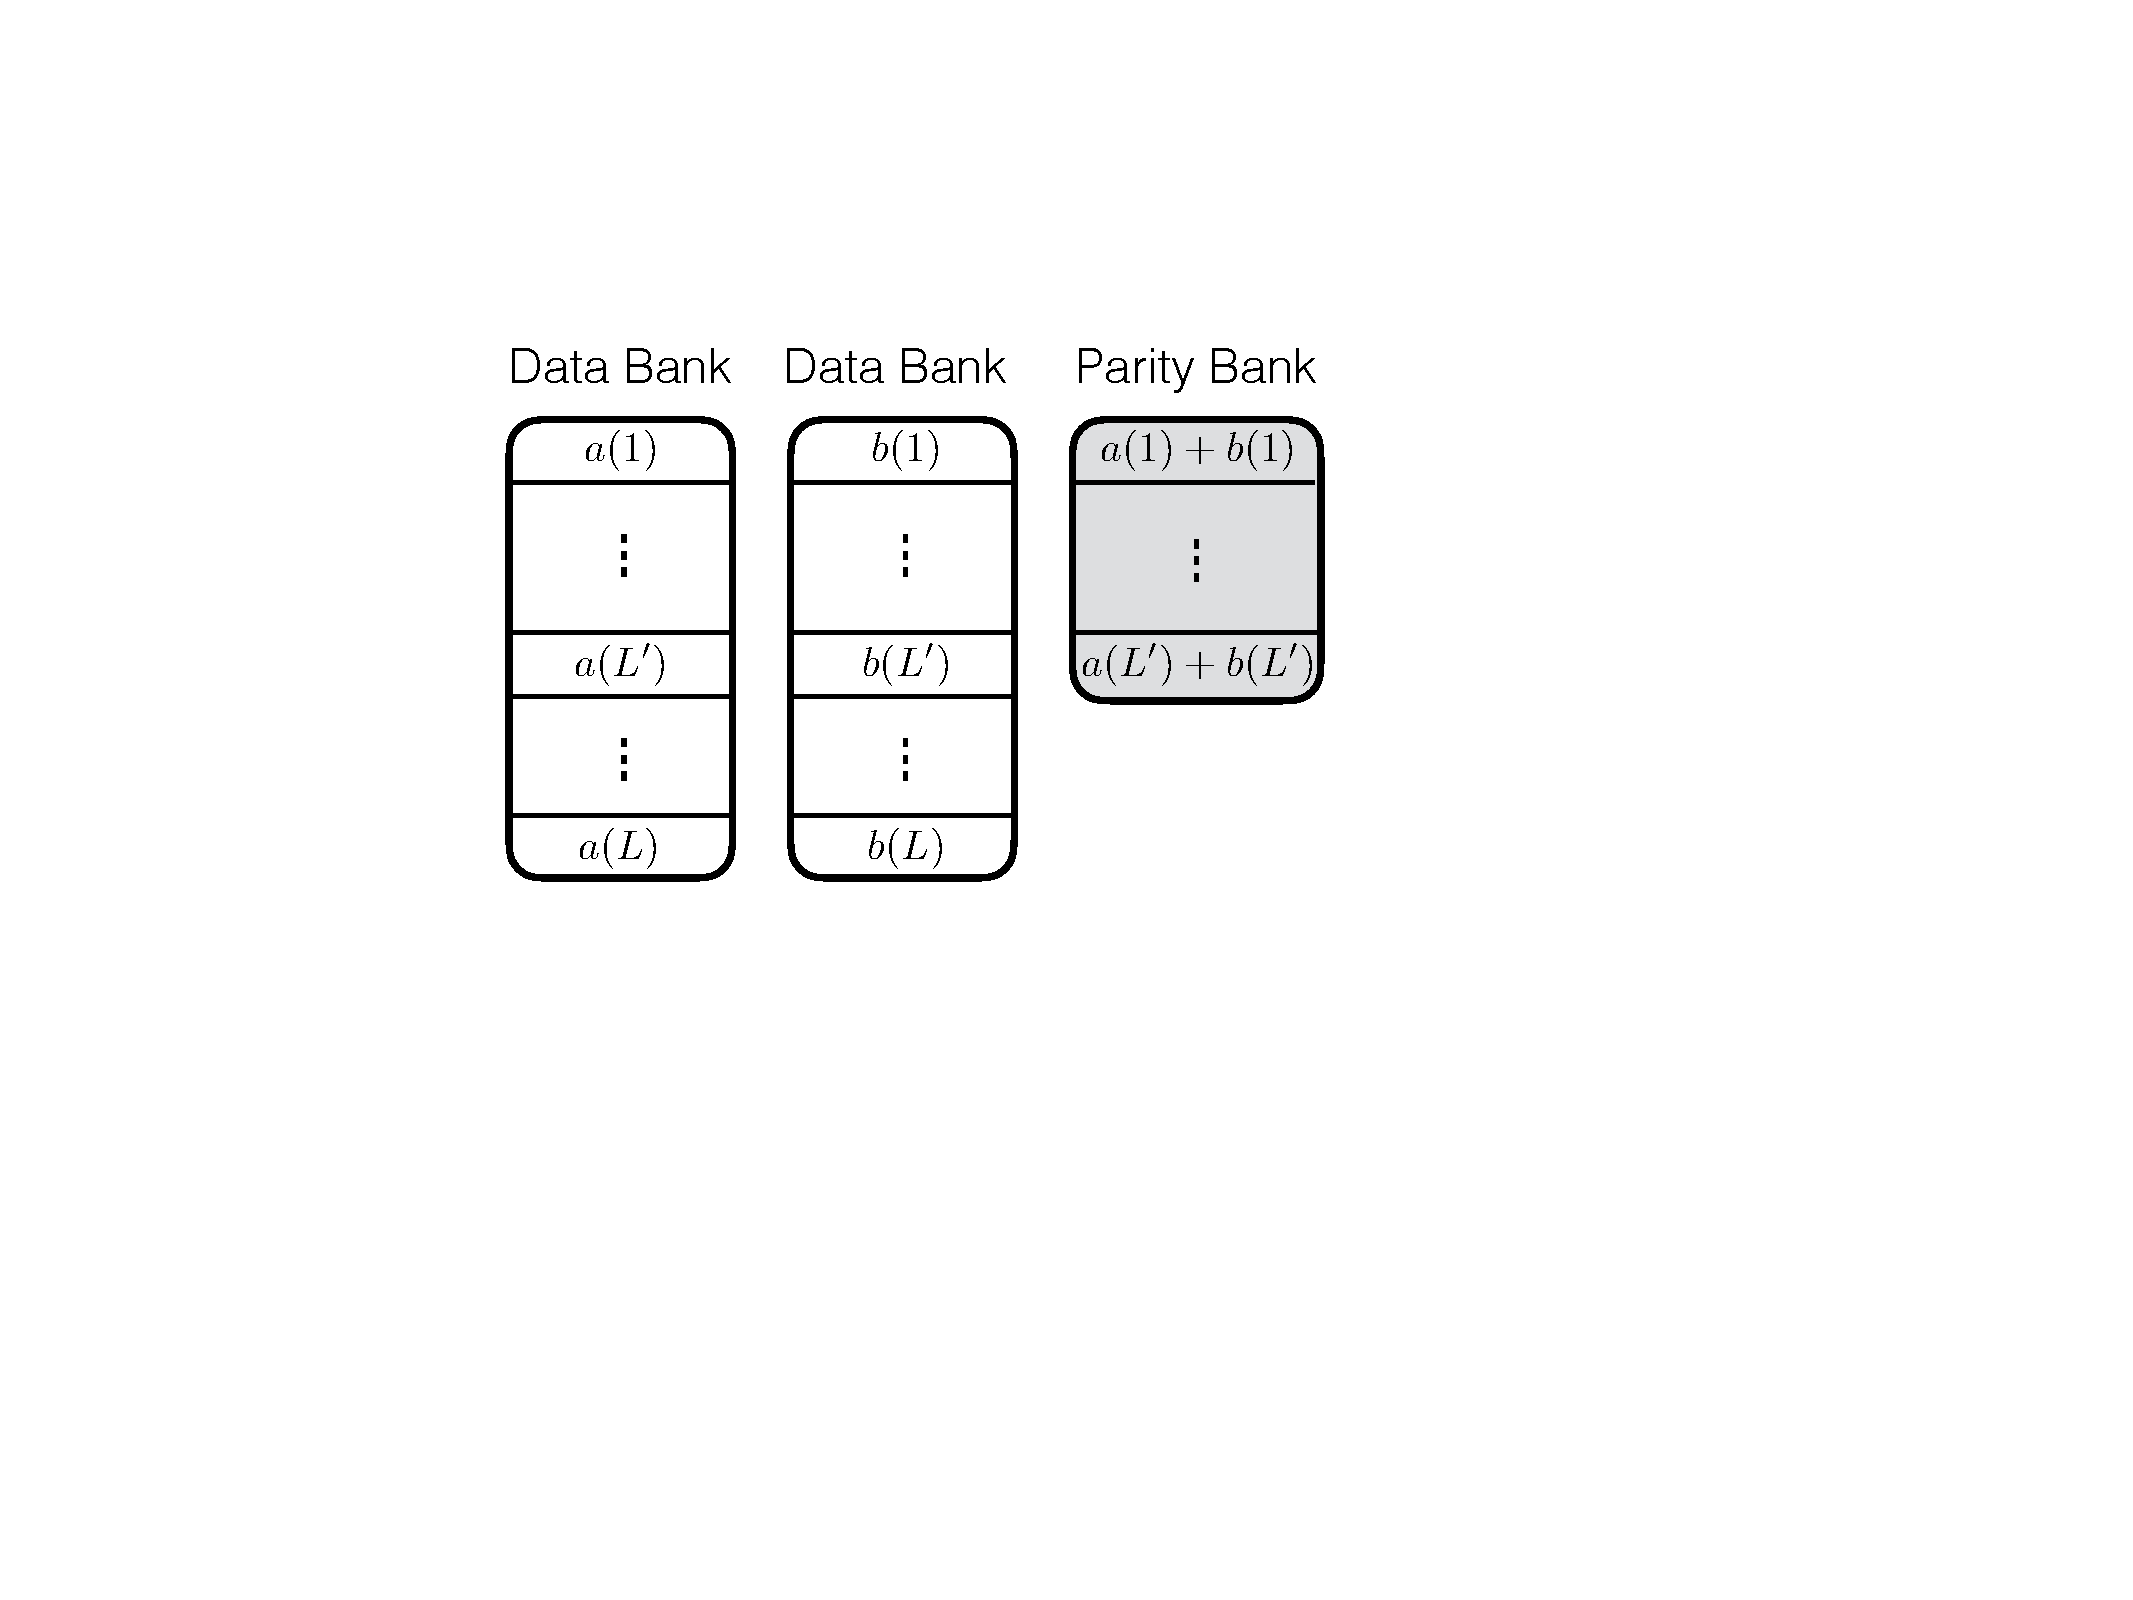
\includegraphics[width=0.95\linewidth]{fig/example-inter-bank.pdf} 
%  \caption{{\color{red}Parity.}}
%  \label{fig:example1_case1}
%\end{subfigure}
%\begin{subfigure}[b]{0.48\linewidth}
%  \centering
%  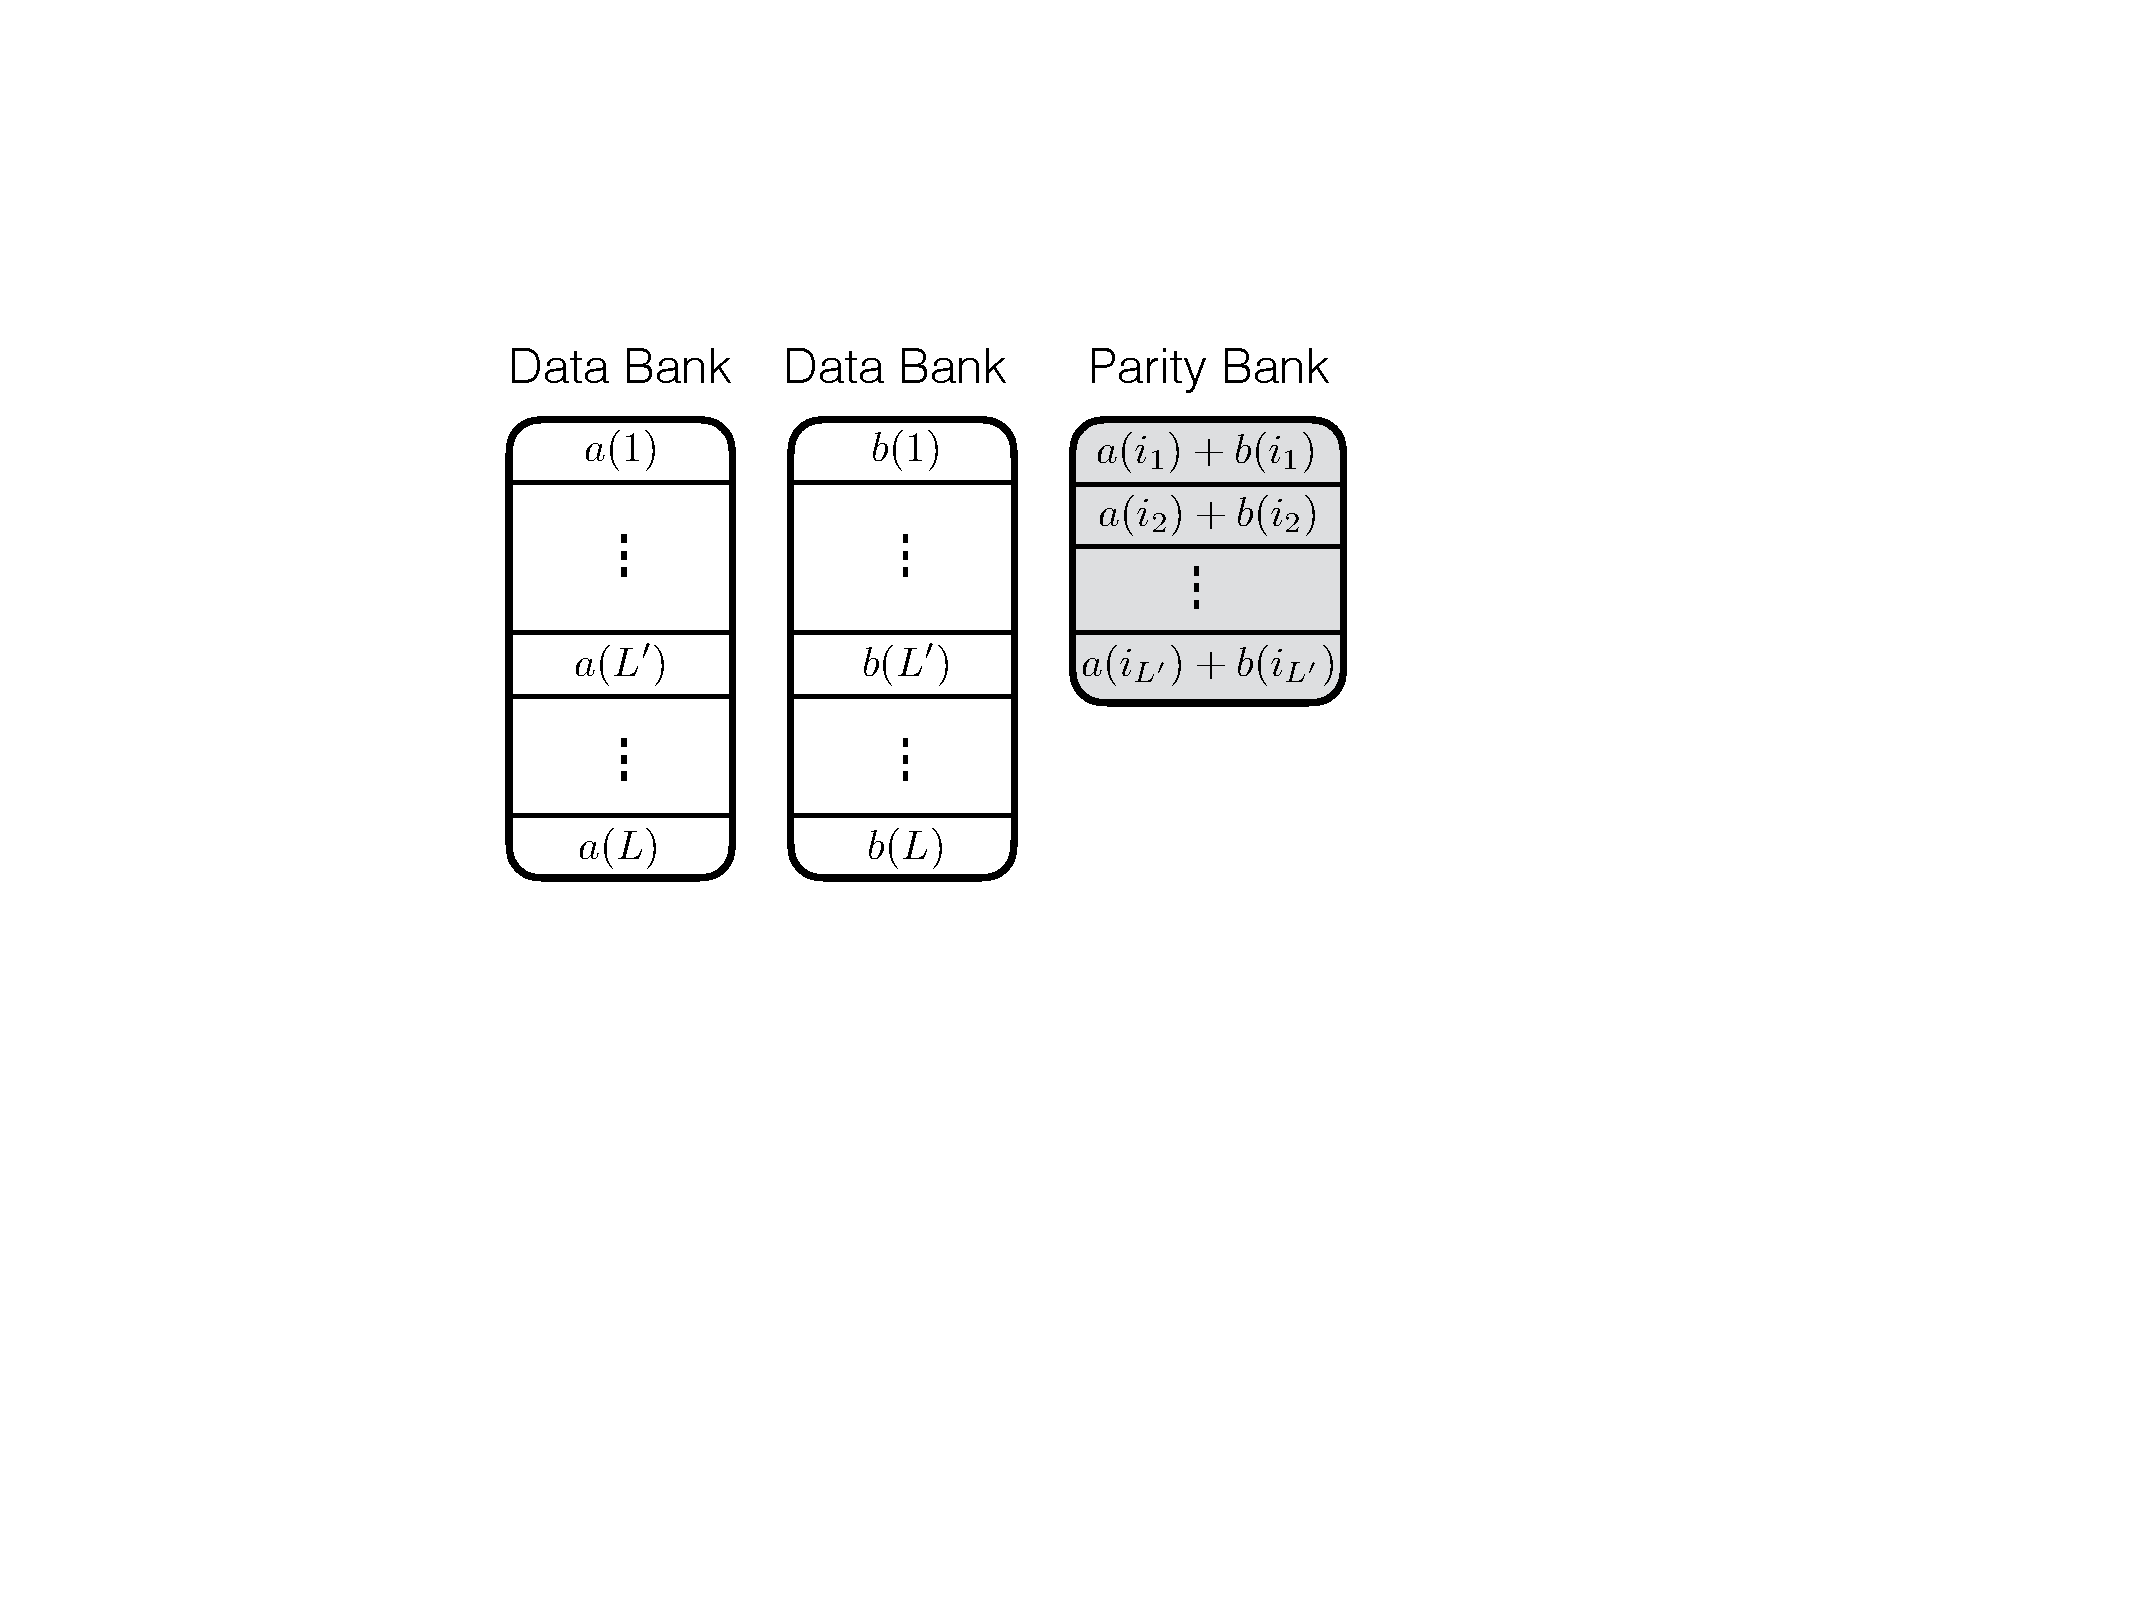
\includegraphics[width=0.98\linewidth]{fig/example-inter-bank-2.pdf} 
%  \caption{{\color{red}Parity.}}
%  \label{fig:example1_case2}
%\end{subfigure}
%\caption{{\color{red}Design.}}
%\label{fig:example1}
%\end{figure}
\begin{figure}[t!]
\centering
  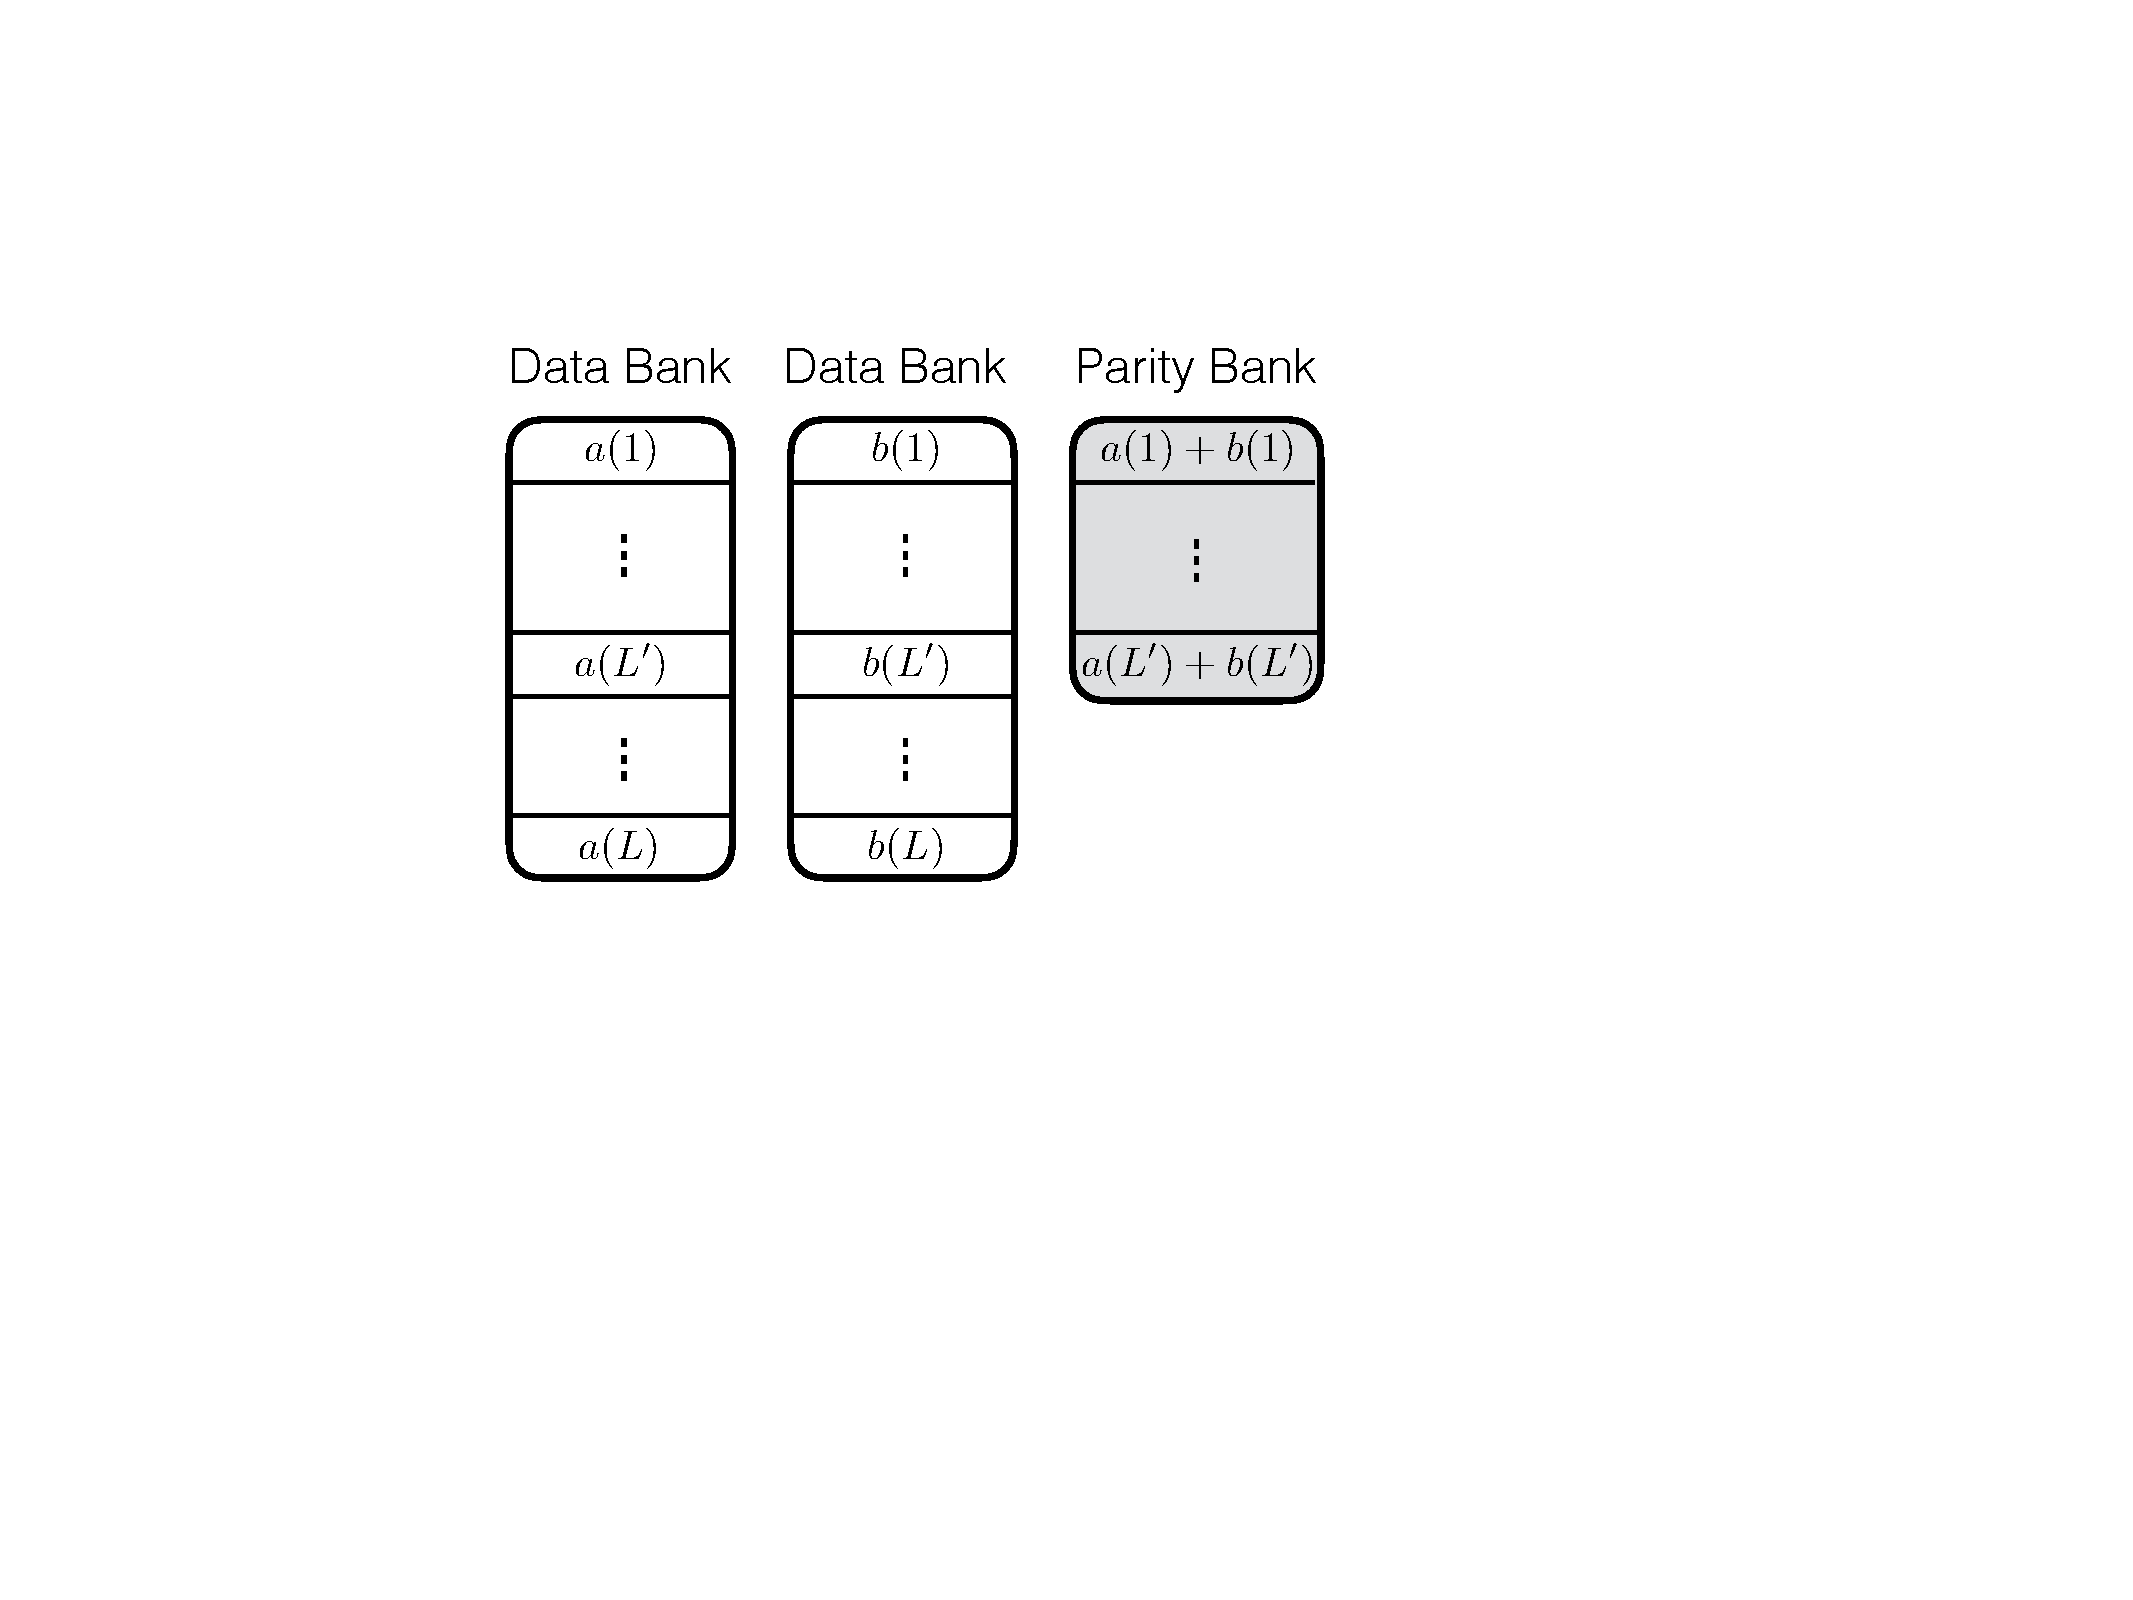
\includegraphics[width=0.45\linewidth]{fig/example-inter-bank.pdf} 
\caption{\it{This illustration is an example parity design.}}
\label{fig:example1}
\end{figure}
%%%%%%%%%%%%%%%%%%%%%%%%%%%%%%%%%%%%%%


\begin{remark}
Note that we allow for the data banks and parity banks to have different sizes, \textit{i.e.} $L \neq L'$. This freedom in memory design can be utilized to reduce the storage overhead of parity banks based on the underlying application. If the size of a parity bank is smaller than a data bank, \textit{i.e.} $L' < L$, we say that the parity bank is a {\em shallow bank}. We note that it is reasonable to assume the existence of shallow banks, especially in proprietary designs of integrated memories in a system on a chip (SoC).
\end{remark}

\begin{remark}
\label{rem:design1}
Note that the size of shallow banks is a design choice which is controlled by the parameter $0 < \alpha \leq 1$. A small value of $\alpha$ corresponds to small storage overhead. The choice of a small $\alpha$ comes at the cost of limiting parity memory accesses to certain memory ranges. In Section~\ref{sec:dynamicCoding} we discuss techniques for choosing which regions of memory to encode. In scenarios where many memory accesses are localized to small regions of memory, shallow banks can support many parallel memory accesses for little storage overhead. For applications where memory access patterns are less concentrated, the robustness of the parity banks allows one to employ a design with $\alpha = 1$.
\end{remark}

\subsubsection{Degraded reads and their locality}
\label{sec:degraded}

The redundant data generated by a coding scheme mitigates bank conflicts by supporting multiple read accesses to the original data elements. Consider the coding scheme illustrated in Figure~\ref{fig:example1} with a parity bank $\mathbf{p} = \mathbf{a}([L']) + \mathbf{b}([L'])$. In an uncoded memory system simultaneous read requests for bank $\mathbf{a}$, such as $a(1)$ and $a(5)$, result in a bank conflict. The introduction of $\mathbf{p}$ allows both read requests to be served. First, $a(1)$ is served directly from bank  $\mathbf{a}$. Next, $b(5)$ and $p(5)$ are downloaded. $a(5) = b(5) + p(5)$, so $a(5)$ is recovered by means of the memory in the parity bank. A read request which is served with the help of parity banks is called a {\em degraded read}. Each degraded read has a parameter {\em locality} associated with it which corresponds to the total number of banks used to serve it. In this case, the degraded read for $a(5)$ using $\mathbf{b}$ and $\mathbf{p}$ has locality $2$.

%In order to further illustrate the notion of locality, let's consider a setup where we generate a parity bank $\mathbf{p}$ by combining three data banks $\mathbf{a}$, $\mathbf{b}$, and $\mathbf{c}$ as $\mathbf{p} = \mathbf{a} + \mathbf{b} + \mathbf{c}$. Now, a degraded read for $a(1)$ using the parity bank as $$a(1) = b(1) + c(1) + p(1) = b(1) + c(1) + \big(a(1) + b(1) + c(1)\big)$$
%has locality $3$ as the degraded read is served using three memory banks.

\subsection{Codes to emulate multi-port memory}
\label{sec:designs}

We will now describe the code schemes proposed for the emulation of multi-port memories. Among a large set of possible coding schemes, we focus on three specific coding schemes for this task. We believe that these three coding schemes strike a good balance among various quantitative parameters, including storage overhead, number of simultaneous read requests supported by the array of banks, and the locality associated with various degraded reads. Furthermore, these coding schemes respect the practical constraint of encoding across a small number of data banks. In particular, we focus on the setup with $8$ memory banks, which contrasts with communications applications where encoding typically occurs with blocks of $1024$ or more information symbols. 

In the rest of this section, we present three code schemes and discuss the number of simultaneous read requests supported by these schemes in the best and worst case. We summarize all the relevant parameters associated with these schemes in Table~\ref{table:codedesigncomparison}.
%
%We discuss the design of the codes for creating extra accesses to memory in this 
%section. First we discuss the code schemes explored during Phase I. Second, we discuss 
%specific execution strategies to efficiently implement the designs.\\
%In the following sub-sections, we discuss 3 designs for storing coded data.  
%Table~\ref{table:codedesigncomparison} compares these designs for various 
%parameters and associated costs.  
%\begin{table*}[t]
%\centering
%	\begin{tabular}{|m{1cm}|m{2 cm}|m{1cm}|m{1cm}|m{1cm}|m{1cm}|m{1cm}|}
%\hline
%Design & Max Read per bank & Max Write per bank & Locality & Rate & Memory 
%Overhead & Logical Complexity \\ \hline
%I & 4 & 2 & 2 & $2/5$ & 1.5 $\alpha$ & Low \\ \hline
%II & 5 & 2 & 2 & $2/5$ & 2.5 $\alpha$ & Medium \\ \hline
%III & 4 & 2 & 3 & $1/2$ & \text{      } $\alpha$ & Medium \\ \hline
%	\end{tabular}
%	\caption{Comparison of design with respect to the performance parameters 
%	and associated cost}
%	\label{table:codedesigncomparison}
%\end{table*}


%\begin{tiny}
%\begin{table}[t!]
%  \centering
%  \begin{tabular}{|c|c|c|c|c|c|c|}
%    \hline
%    \textbf{Design} & \textbf{Max reads} & \textbf{Max writes} & \textbf{Locality} & \textbf{Rate} & \textbf{Storage overhead} & \textbf{Logical complexity} \\
%    & \textbf{(per bank)} & \textbf{(per bank)} & & & & \\
%    \hline
%    \hline
%    I & 4 & 2 & 2 & $2/5$ & 1.5 $\alpha$ & Low \\ \hline
%II & 5 & 2 & 2 & $2/5$ & 2.5 $\alpha$ & Medium \\ \hline
%III & 4 & 2 & 3 & $1/2$ & \text{      } $\alpha$ & Medium \\ 
%\hline                                   
%  \end{tabular}
%	\caption{Comparison of the code schemes with respect to the performance parameters and associated cost}
%	\label{table:codedesigncomparison}
%\end{table}
%\end{tiny}

\begin{comment}
\begin{table}[t!]
  \centering
  \begin{tabular}{|c|c|c|c|c|c|}
    \hline
   {\small Design} & {\small  Max reads} &{\small  Locality} & {\small  Rate} & {\small  Storage} & {\small  Logical } \\
    & {\small  (per bank)} & & &{\small  overhead} & {\small  complexity} \\
    \hline
    \hline
    {\small I} & {\small$4$ } & {\small$2$} & {\small ${2}/{5}$} & {\small $1.5\alpha$} & {\small Low} \\ \hline
{\small II} & {\small$5$}  & {\small$2$} & {\small ${2}/{5}$} & {\small $2.5\alpha$} & {\small Medium} \\ \hline
{\small III }& {\small$4$}  & {\small$3$} & {\small$1/2$} & {\small $\alpha$} & {\small Medium} \\ 
\hline                                   
  \end{tabular}
	\caption{\it{Comparison of the code schemes with respect to the performance parameters and associated cost. $\alpha$ is the fraction of storage overhead in comparison to the data bank. $\alpha = 1$ when size of parity bank is equal to size of data bank.}}
	\label{table:codedesigncomparison}
\end{table}
\end{comment}

\begin{table}[ht!]
  \centering
  \begin{tabular}{|c|c|c|c|c|c|}
    \hline
   {\scriptsize Design} & {\scriptsize  Max reads} &{\scriptsize  Locality} & {\scriptsize  Rate} & {\scriptsize  Storage} & {\scriptsize  Logical } \\
    & {\scriptsize  (per bank)} & & {\scriptsize ($\alpha=1$)}&{\scriptsize  overhead} & {\scriptsize  complexity} \\
    \hline
    \hline
    {\scriptsize I} & {\scriptsize$4$} & {\scriptsize$2$} & {\scriptsize $\nicefrac{2}{5}$} & {\scriptsize $1.5\alpha$} & {\scriptsize Low} \\ \hline
%{\scriptsize II} & {\scriptsize$5$}  & {\scriptsize$2$} & {\scriptsize ${2}/{5}$} & {\scriptsize $2.5\alpha$} & {\scriptsize Medium} \\ \hline
{\scriptsize II} & {\scriptsize$5$}  & {\scriptsize$2$} & {\scriptsize $\nicefrac{2}{7}$} & {\scriptsize $2.5\alpha$} & {\scriptsize Medium} \\ \hline
{\scriptsize III }& {\scriptsize$4$}  & {\scriptsize$3$} & {\scriptsize$\nicefrac{1}{2}$} & {\scriptsize $\alpha$} & {\scriptsize Medium} \\ 
\hline                                   
  \end{tabular}
	\caption{\it{Comparison of the code schemes with respect to the performance parameters and associated cost.}}
	\label{table:codedesigncomparison}
\end{table}


\subsubsection{Code Scheme I}
\label{sec:design1}

This code scheme is motivated from the concept of batch codes~\cite{batchcodes} which enables parallel access to content stored in a large scale distributed storage system.
%The coding scheme is illustrated in Figure~\ref{fig:design1}. 
The code scheme involves $8$ data banks $\{\mathbf{a}, \mathbf{b},\ldots, \mathbf{h}\}$ each of size $L$ and $12$ shallow banks each of size $L' = \alpha L$. We partition the $8$ data banks into two  groups of $4$ banks. The underlying coding scheme produces shallow parity banks by separately encoding data banks from the two groups. Figure~\ref{fig:design1} shows the resulting memory banks. The storage overhead of this schemes is $12\alpha L$ which implies the rate\footnote{The information rate is a standard measure of redundancy of a coding scheme ranging from $0$ to $1$, where $1$ corresponds to the most efficient utilization of storage space.} of the coding scheme is $$\frac{8L}{8L + 12\alpha L} = \frac{2}{2 + 3\alpha}.$$


We now analyze the number of simultaneous read requests that can be supported by this code scheme. \\
%This allows us to serve multiple accesses to the coded 
%region using the parity banks. With this scheme, we guarantee that any 4 read 
%requests to the coded region can be served at any given time. As shown in 
%figure~\ref{fig:design1}, 8 banks are divided into two regions.  Each region 
%consists of 4 banks. Each region has 6 parallel shallow  banks to store the 
%parity. The colored regions shown in the banks 1-8 are the coded region. These 
%regions are assumed to be of $\alpha $ fraction of the memory. \\

\noindent \textbf{Best case analysis:~}This code scheme achieves maximum 
performance when sequential accesses to the coded regions are issued. During the 
best case access, we can achieve up to $10$ parallel accesses to a particular coded region in one access cycle.
Consider the scenario when we receive accesses to the following $10$ rows:
\begin{align*}
&\left\{a(1),b(1),c(1),d(1),a(2),b(2),c(2),d(2),c(3),d(3)\right\} .
\end{align*}
Note that we can serve the read requests for the rows \\ $\{a(1),b(1),c(1),d(1)\}$ using the data bank $\mathbf{a}$ and the three parity banks storing $\{a(1)+b(1), b(1)+c(1),c(1)+d(1)\}$. The requests for $\{a(2),c(2),d(2)\}$ can be served by downloading $b(2)$ from the data bank $\mathbf{b}$ and $\{a(2)+d(2), b(2)+d(2),a(2)+c(2)\}$ from their respective parity banks. Lastly, in the same memory clock cycle, we can serve the requests for $\{c(3), d(3)\}$ using the data banks $\mathbf{c}$ and $\mathbf{d}$.\\
%------------------------------
\begin{figure}[ht!]
\centering
	%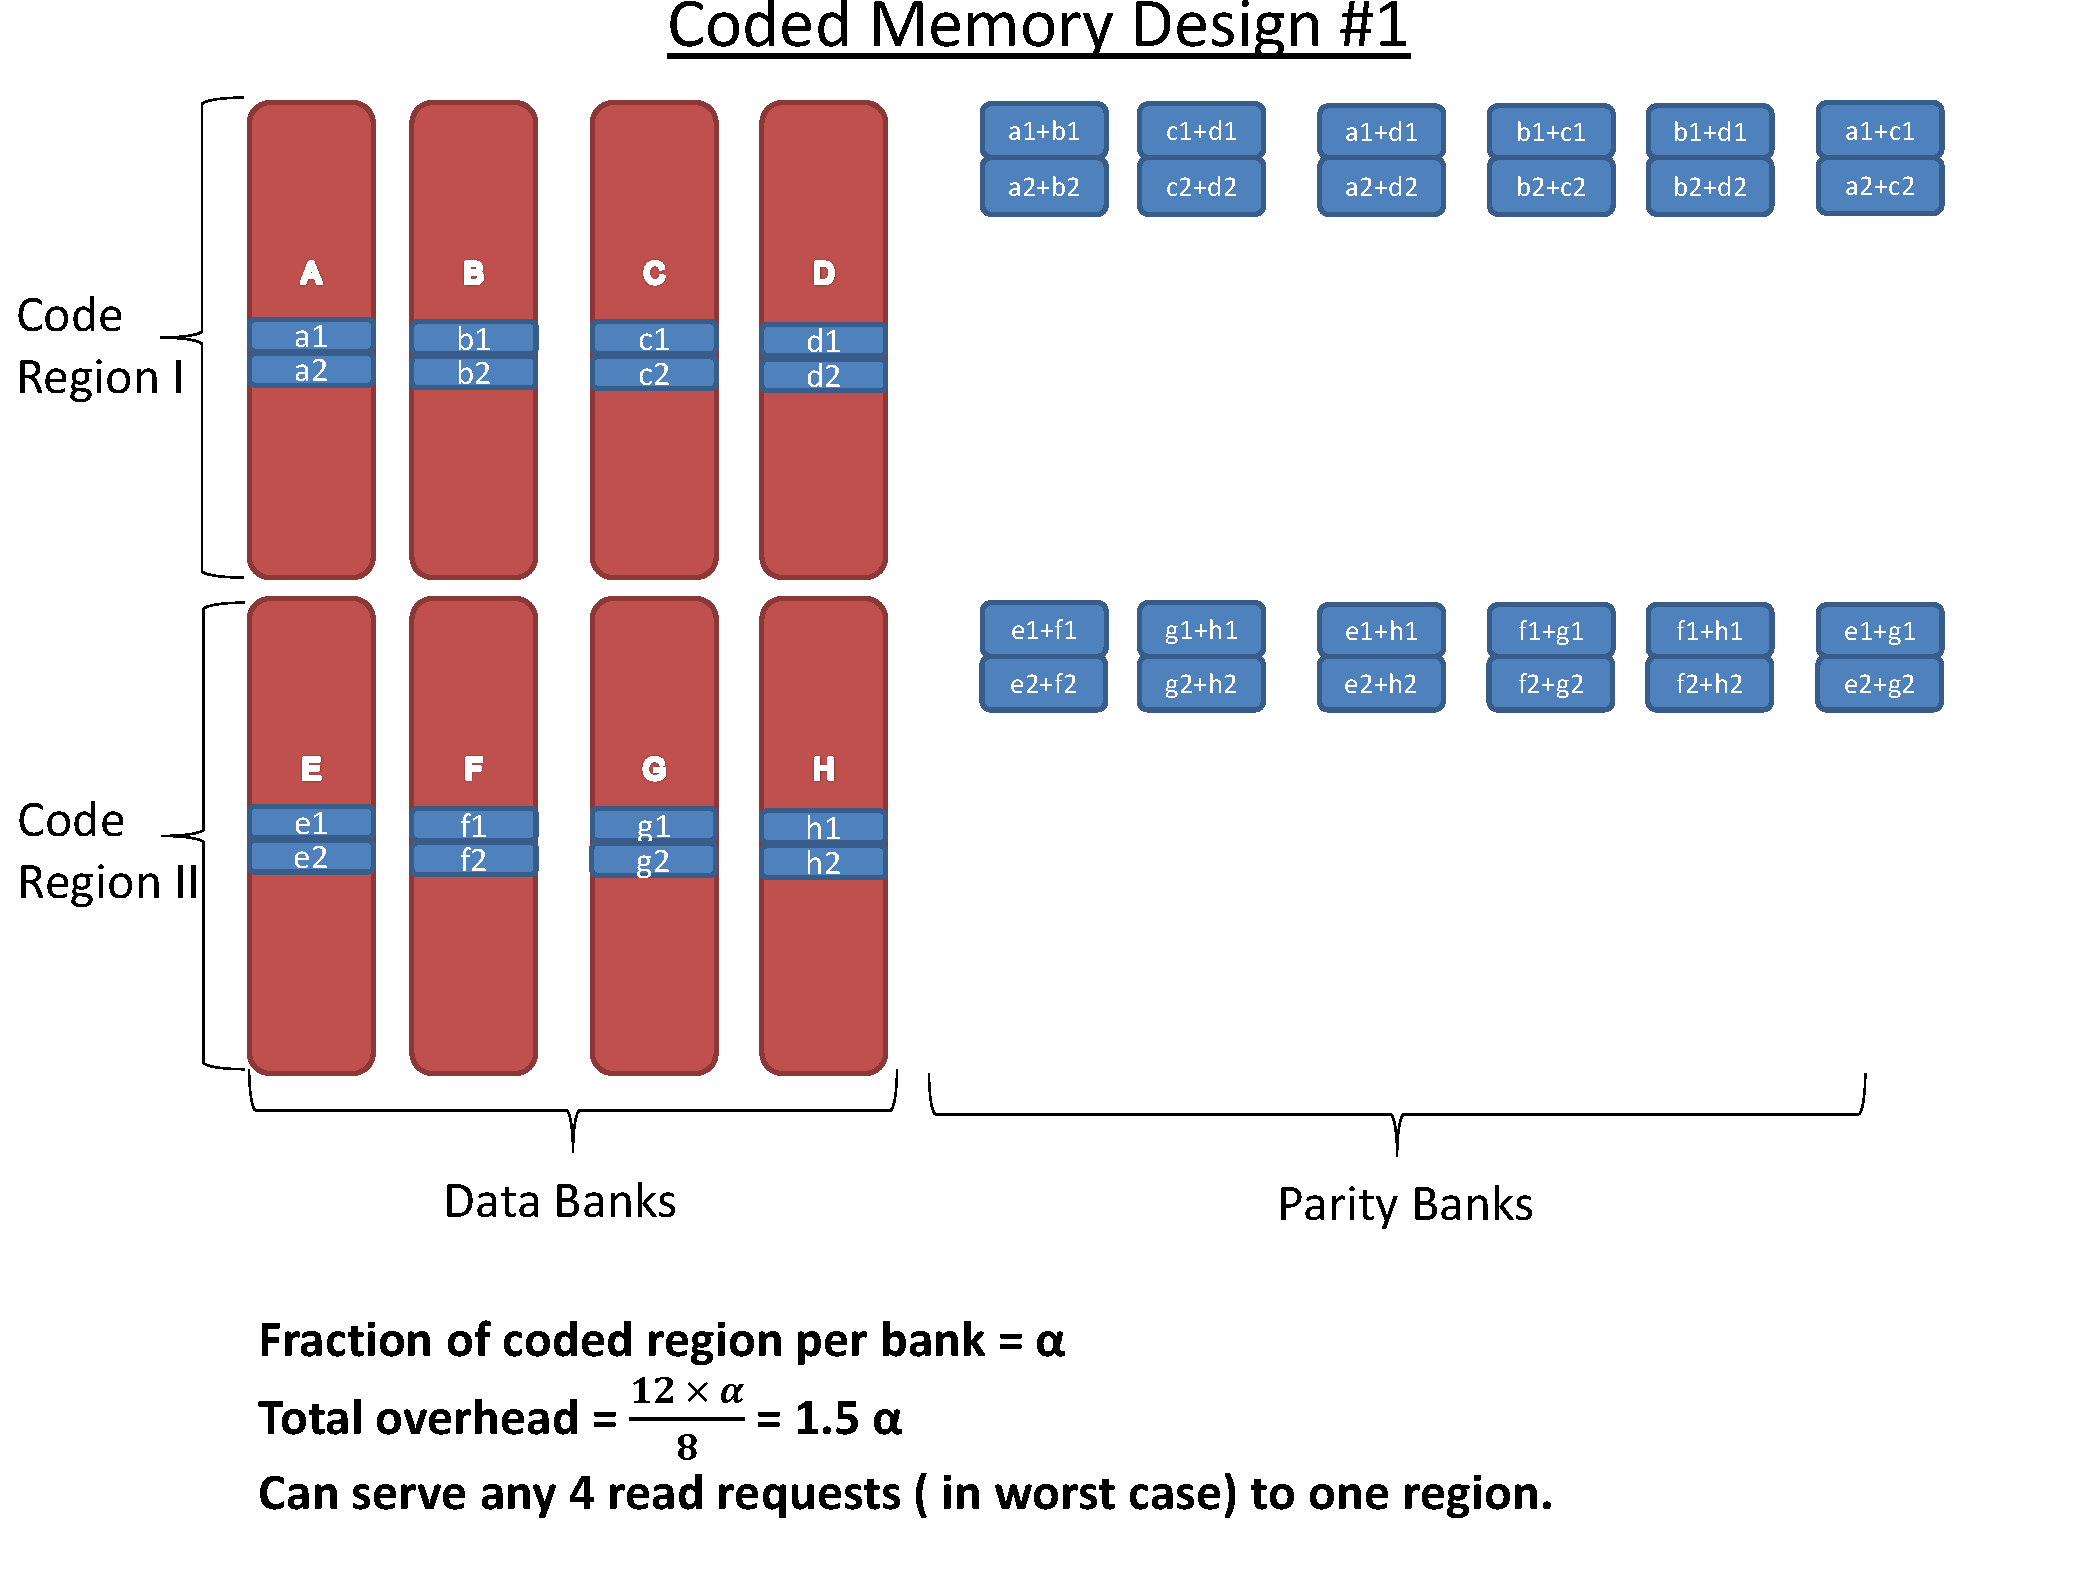
\includegraphics[width=0.8\linewidth]{fig/designI.pdf}
	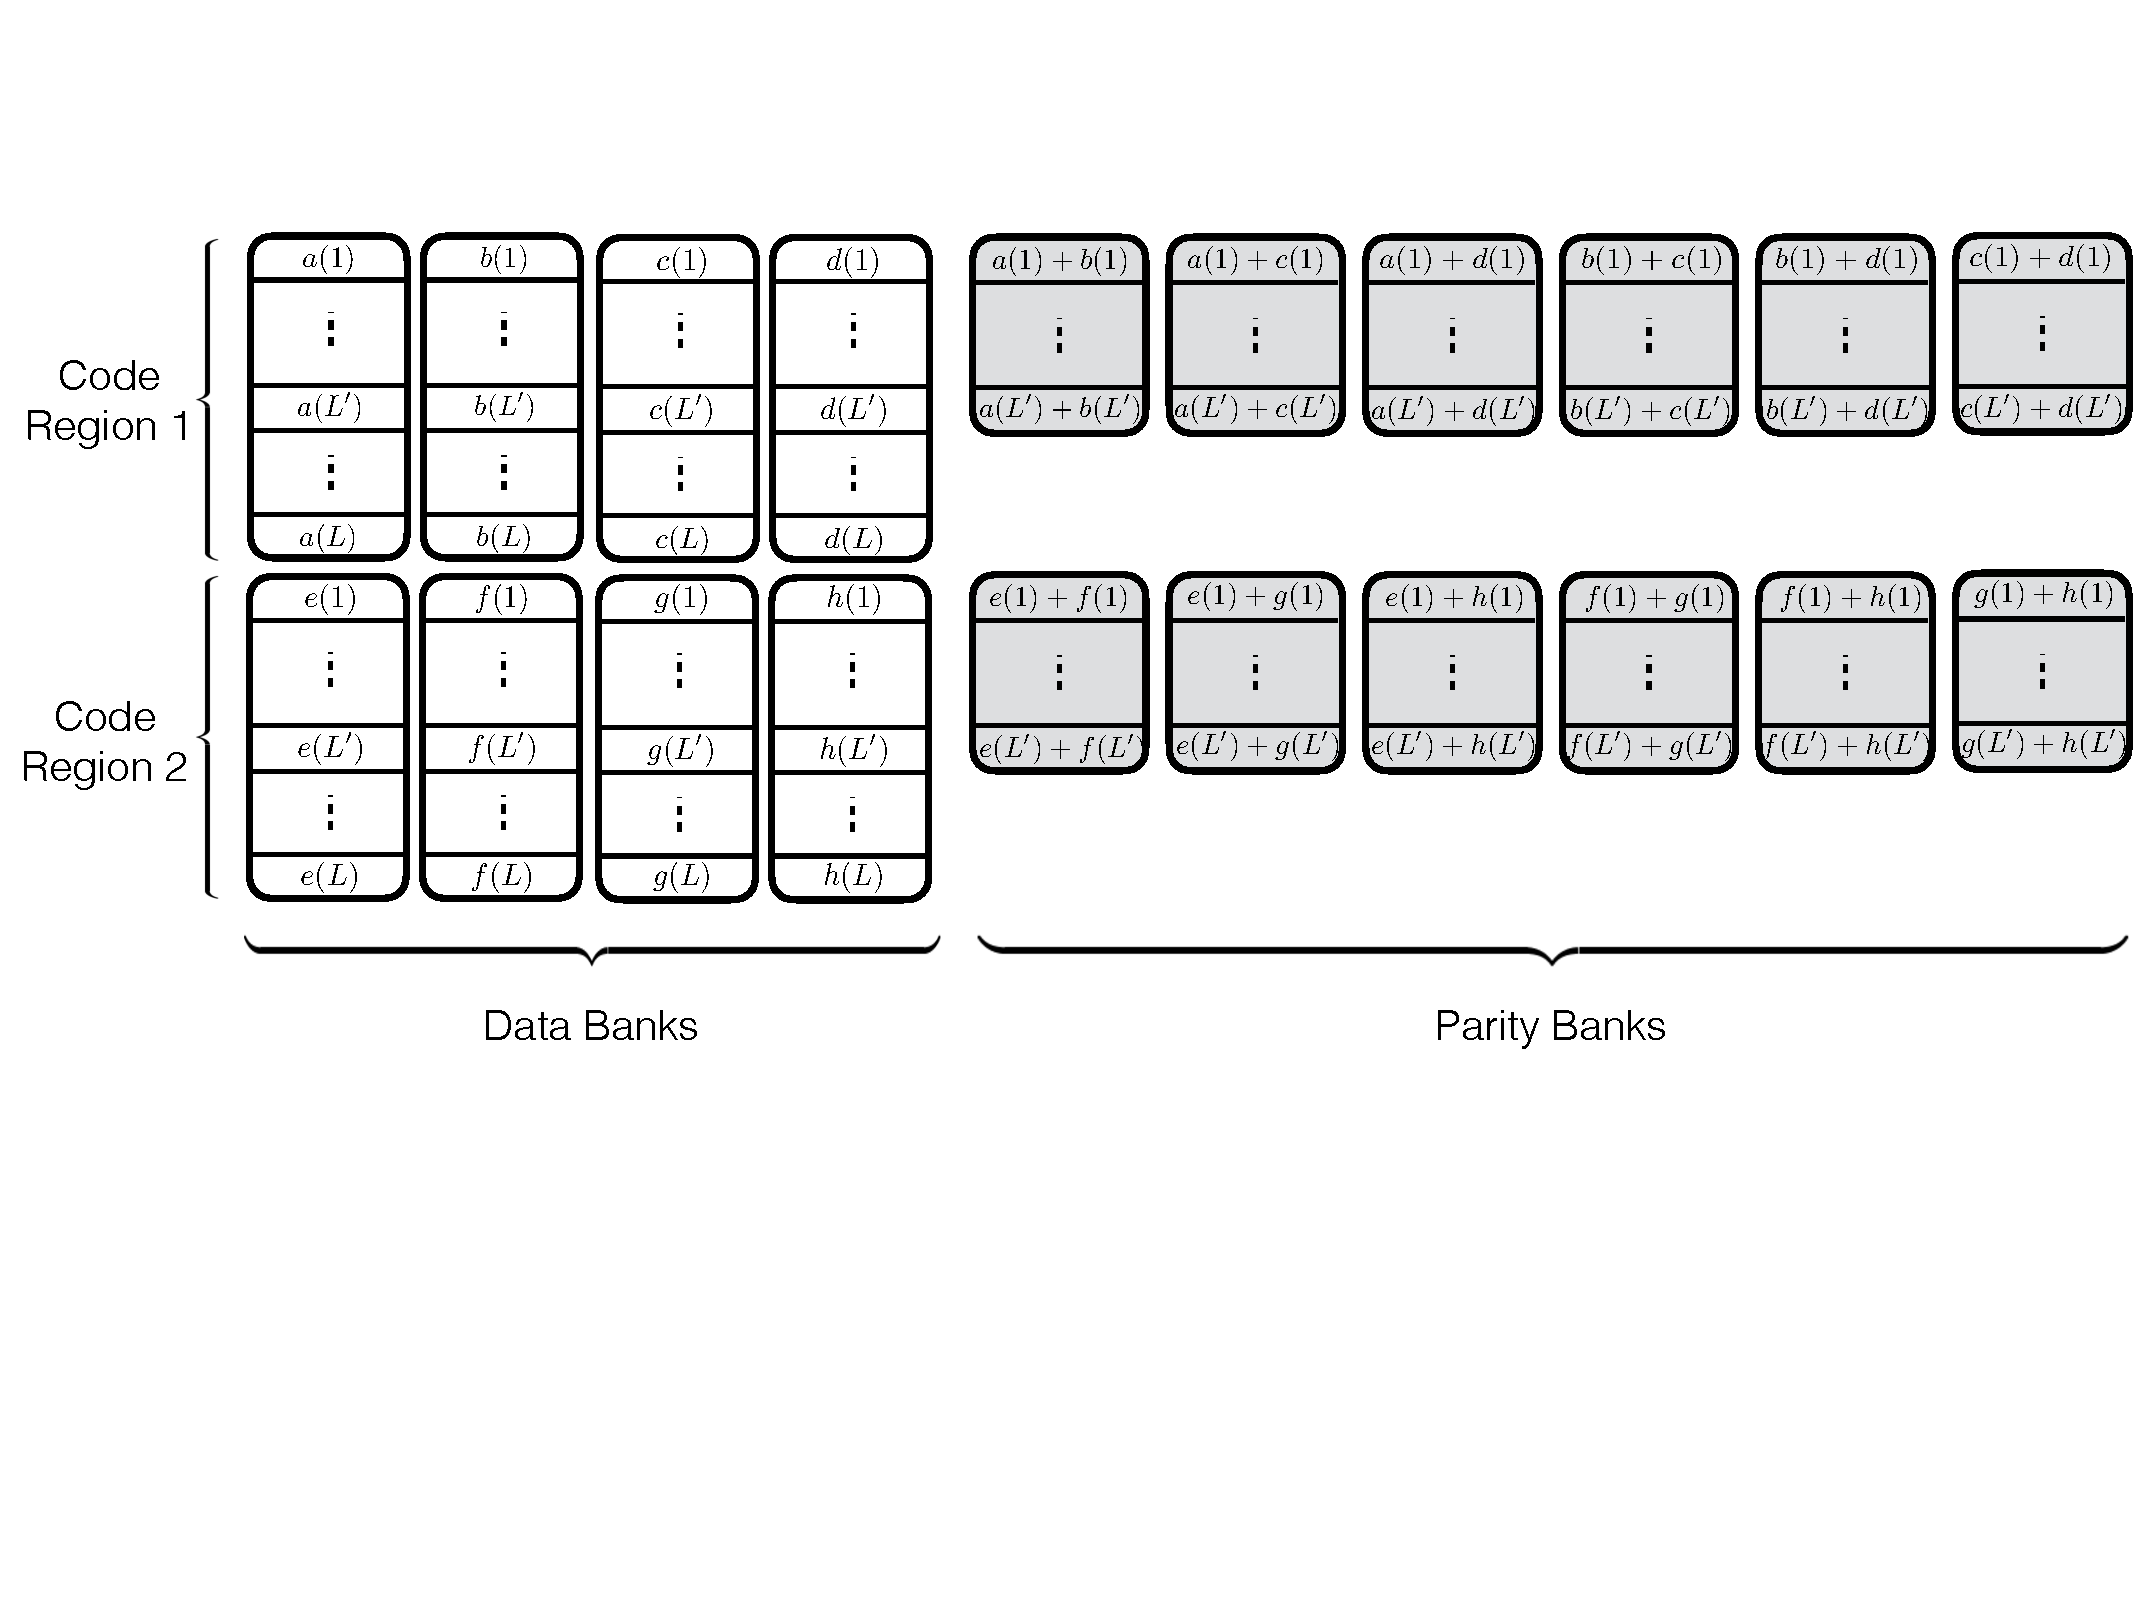
\includegraphics[width=1\linewidth]{fig/Code-Design-1.pdf}
	\caption{\it{Pictured here is an illustration of code scheme I.}}
	\label{fig:design1}
%\caption{Code Schemes}
\end{figure} 
%------------------------------
\ignore{
%------------------------------
\begin{figure}[ht!]
\centering
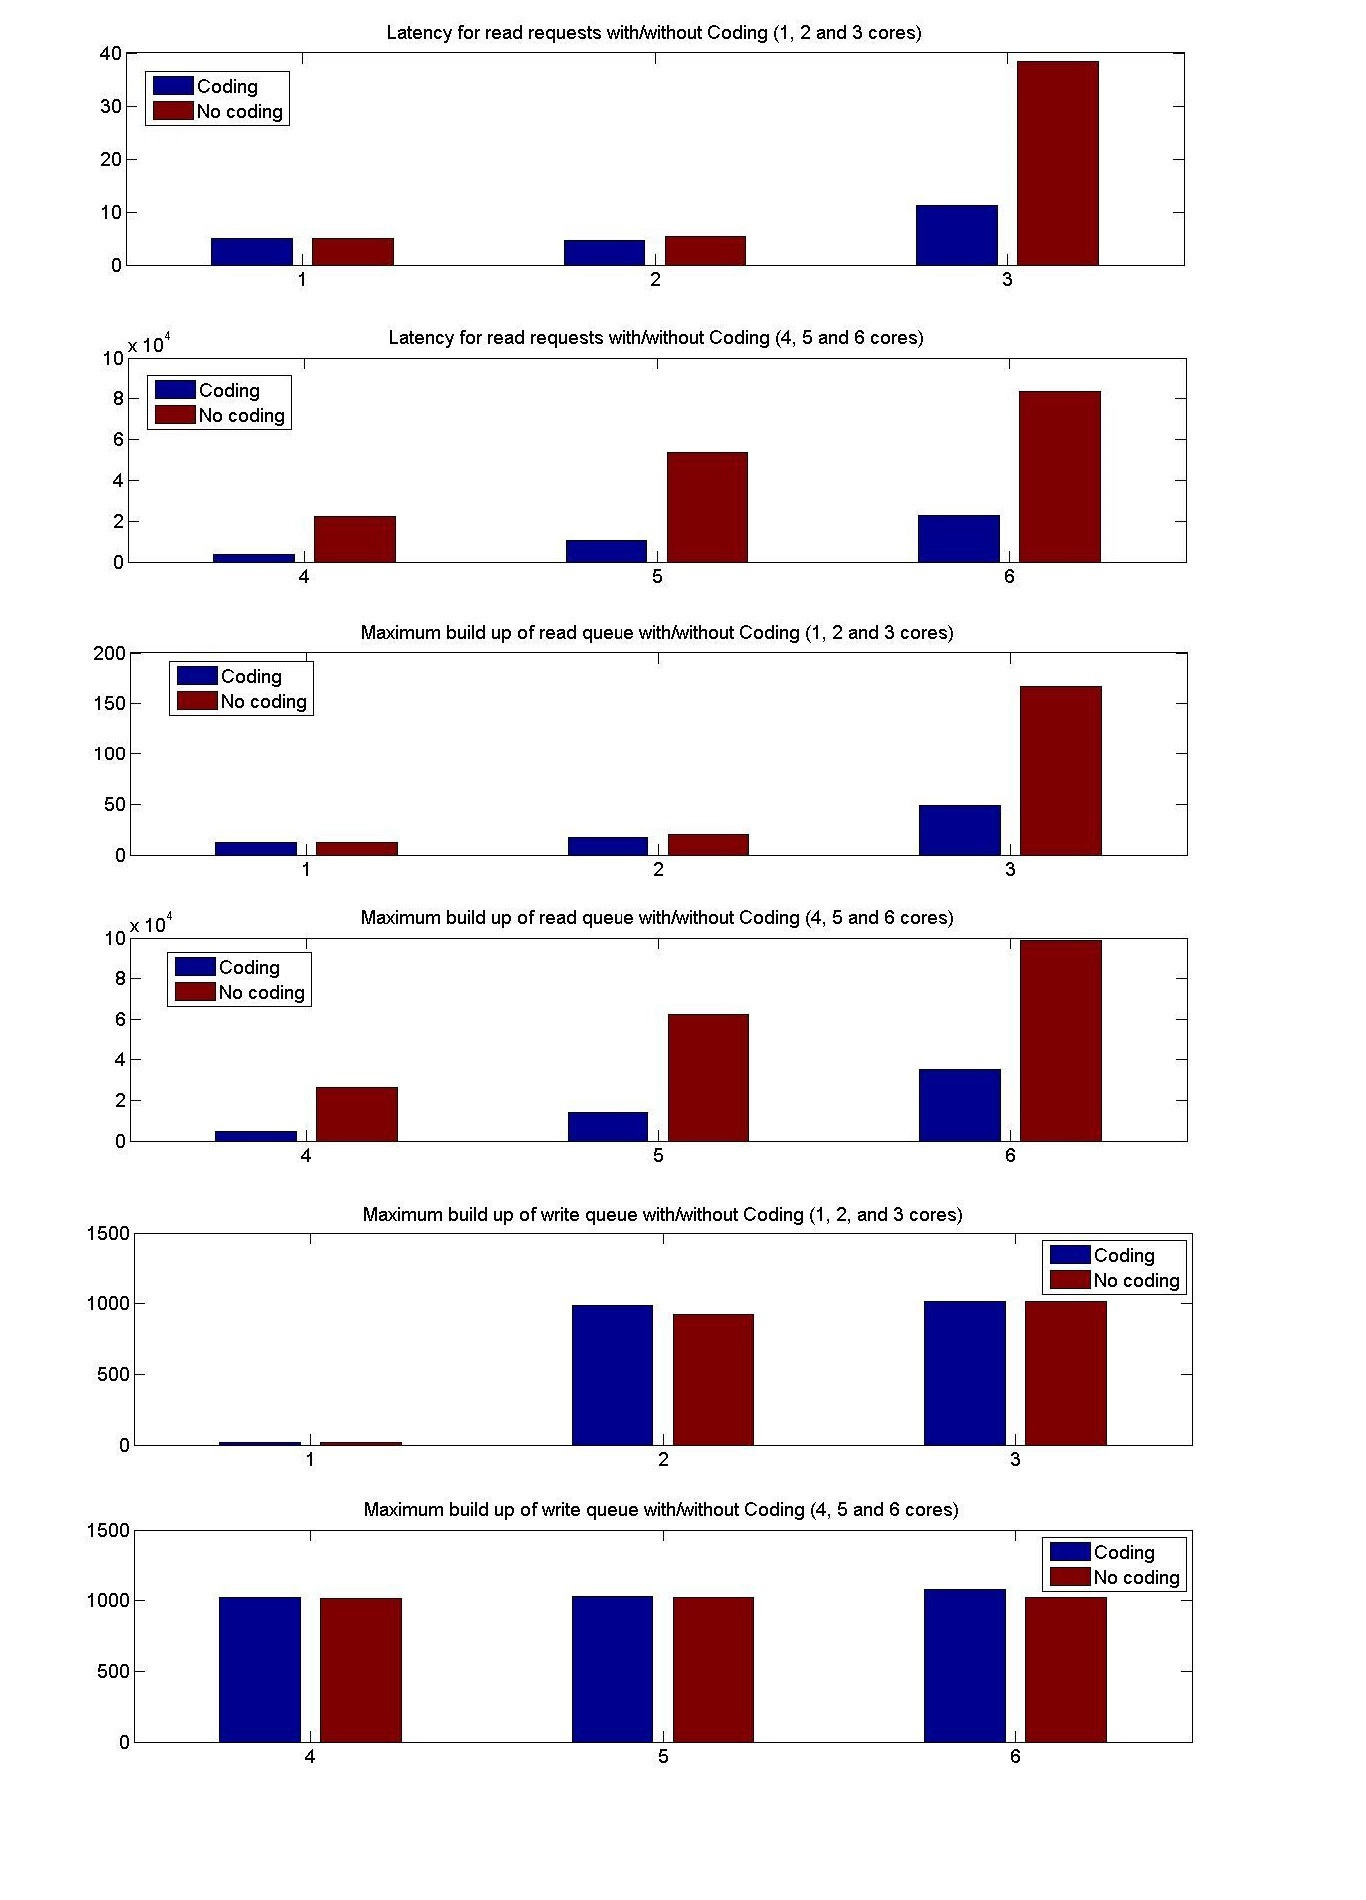
\includegraphics[width=150mm,natwidth=610,natheight=642]{fig/result_design1.jpg}
\caption{ }
\label{fig:result_design1}
\end{figure}
%------------------------------
}
\noindent \textbf{Worst case analysis}: This code scheme  (cf.~Figure~\ref{fig:design1}) may fail to utilize any parity banks depending on the requests waiting to be served. The worst case scenario for this code scheme is when there are non-sequential and non-consecutive access to the memory 
banks. Take for example a scenario where we only consider the first four banks of the code scheme. The following read requests are waiting to be served:  
\begin{align*}
\{a(1), a(2), b(8), b(9), c(10),c(11), d(14), d(15)\}. 
\end{align*}
Because none of the requests share the same row index, we are unable to utilize the parity banks. However, we still benefit from the prefetching mechanism discussed in Section~\ref{sec:prefetching}. The worst case number of reads per cycle is equal to the number of data banks. 
%In Figure~\ref{fig:result_design1} , we explore the worst case scenario when 
%the accesses are random. The results show that the queue build up for reads and 
%writes does fall back to no-coding scenario. This asserts that the worst case 
%scenario for a coding scheme performs similar to no-coding scheme.In the second 
%scheme, we augment the code storage by cross storing the codes from region 1 to 
%region 2 and vice-versa.We do this in addition to coding the consecutive memory 
%addresses in a bank. This provides two benefits, first it increases the overall 
%redundancy, and second it allows us to use the parity banks of the other region 
%in case the first region�s parity banks are in use. 
\ignore{
\begin{figure}[!ht]
\centering
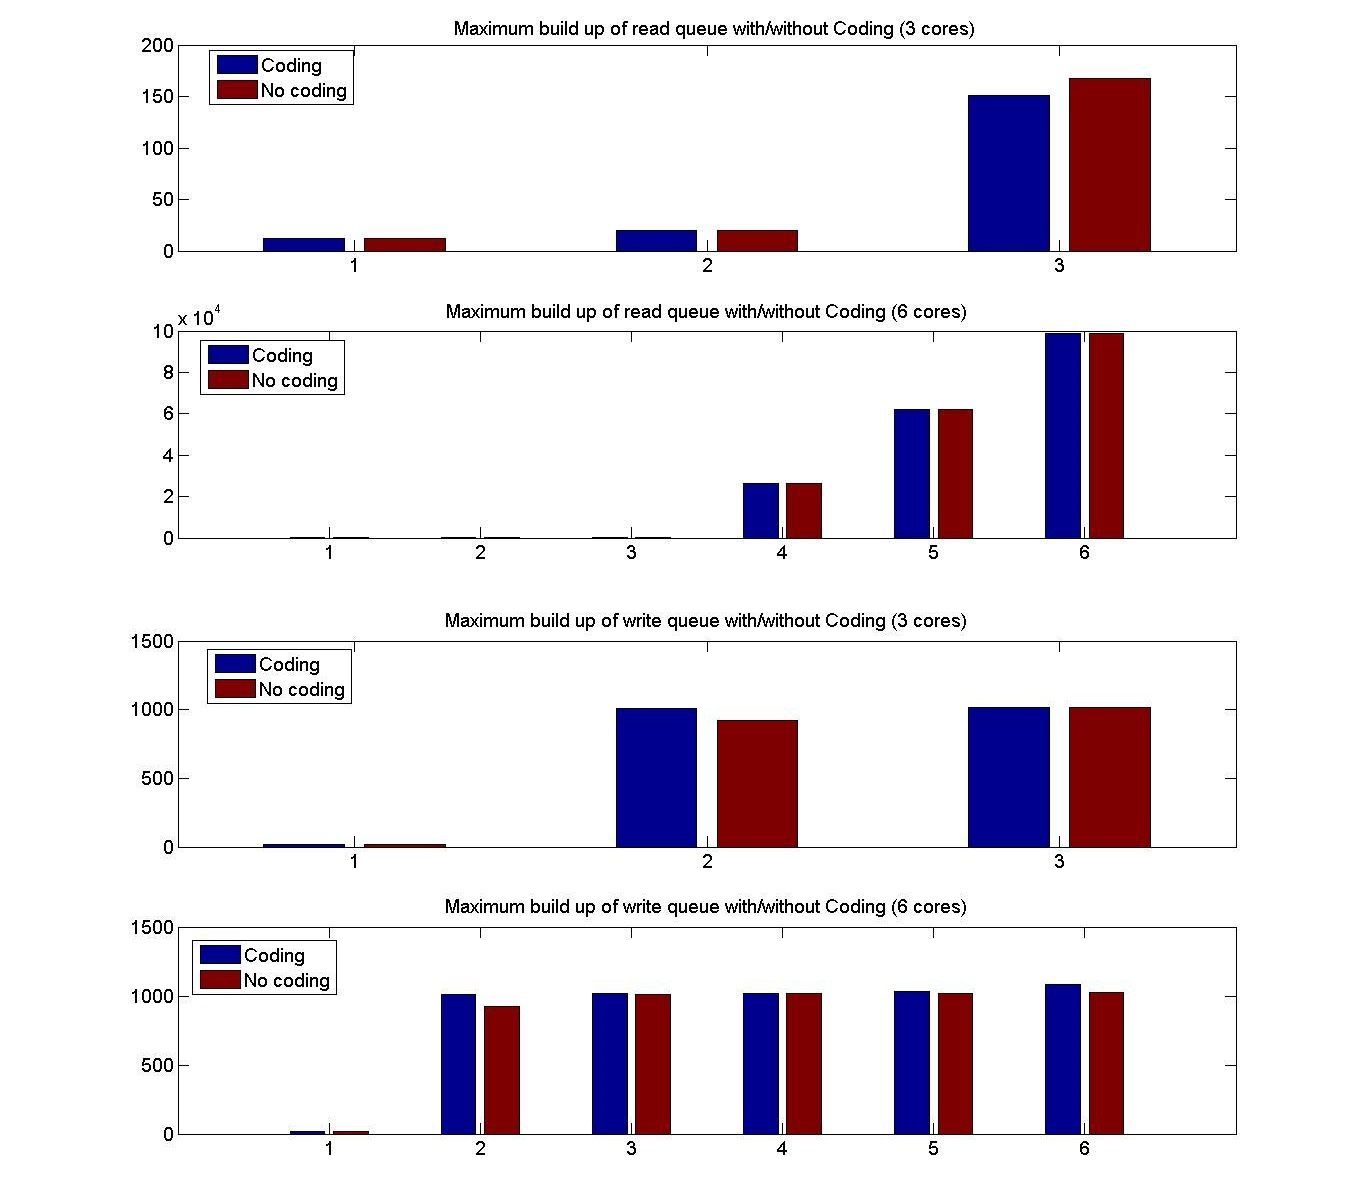
\includegraphics[width=150mm,natwidth=610,natheight=642]{fig/result_design2.jpg}
\caption{ Comparison of Design II with No coding case }
\label{fig:result_design2}
\end{figure}
}
\subsubsection{Code Scheme II}
\label{sec:design2}

Figure~\ref{fig:design2} illustrates the second code scheme explored in this paper. Again, the $8$ data banks $\{\mathbf{a}, \mathbf{b},\ldots, \mathbf{h}\}$ are partitioned into two groups containing $4$ data banks each. These two groups are then associated with two code regions. The first code region is similar to the previous code scheme, as it contains parity elements constructed from two data banks. The second code region contains data directly duplicated from single data banks. This code scheme further differs from the previous code scheme (cf. Figure~\ref{fig:design1}) in terms of the size and arrangement parity banks. Even though $L' = \alpha L$ rows from each data bank are stored in a coded manner by generating parity elements, the parity banks are assumed to be storing $2\alpha L > L'$ rows.

For a specific choice of $\alpha$, the storage overhead of this scheme is $20\alpha L$ which leads to a rate of $$\frac{8L}{8L + 20\alpha L} = \frac{2}{2 + 5\alpha}.$$ Note that this code scheme can support $5$ read accesses per data bank in a single memory clock cycle as opposed to $4$ read requests supported by the code scheme from Section~\ref{sec:design1}. However, this is made possible at the cost of extra storage overhead. Next, we discuss the performance of this code scheme in terms of the number of simultaneous read requests that can be served in the best and worst case.

%
%The second design, presented in figure 4, improves over first design by allowing 
%5 read accesses per bank per cycle. This design also divides banks into two 
%regions. The first region is
%Bank 1 to Bank 4 and 5 corresponding Parity banks. The two regions in figure 4 
%are upper 9 banks forming one region and lower 9 banks forming another. This 
%design allows intermix storage of parity among regions. The design uses 5 parity 
%banks per region. The data in this scheme is coded for both inter bank and 
%intra-bank. The intra-bank codes are stored in the alternate parity bank region. 
%This allows usage of parity banks from other region if they are available. \\
\begin{figure}[!ht]
%\centering
%\begin{minipage}[!t]{\linewidth}
	%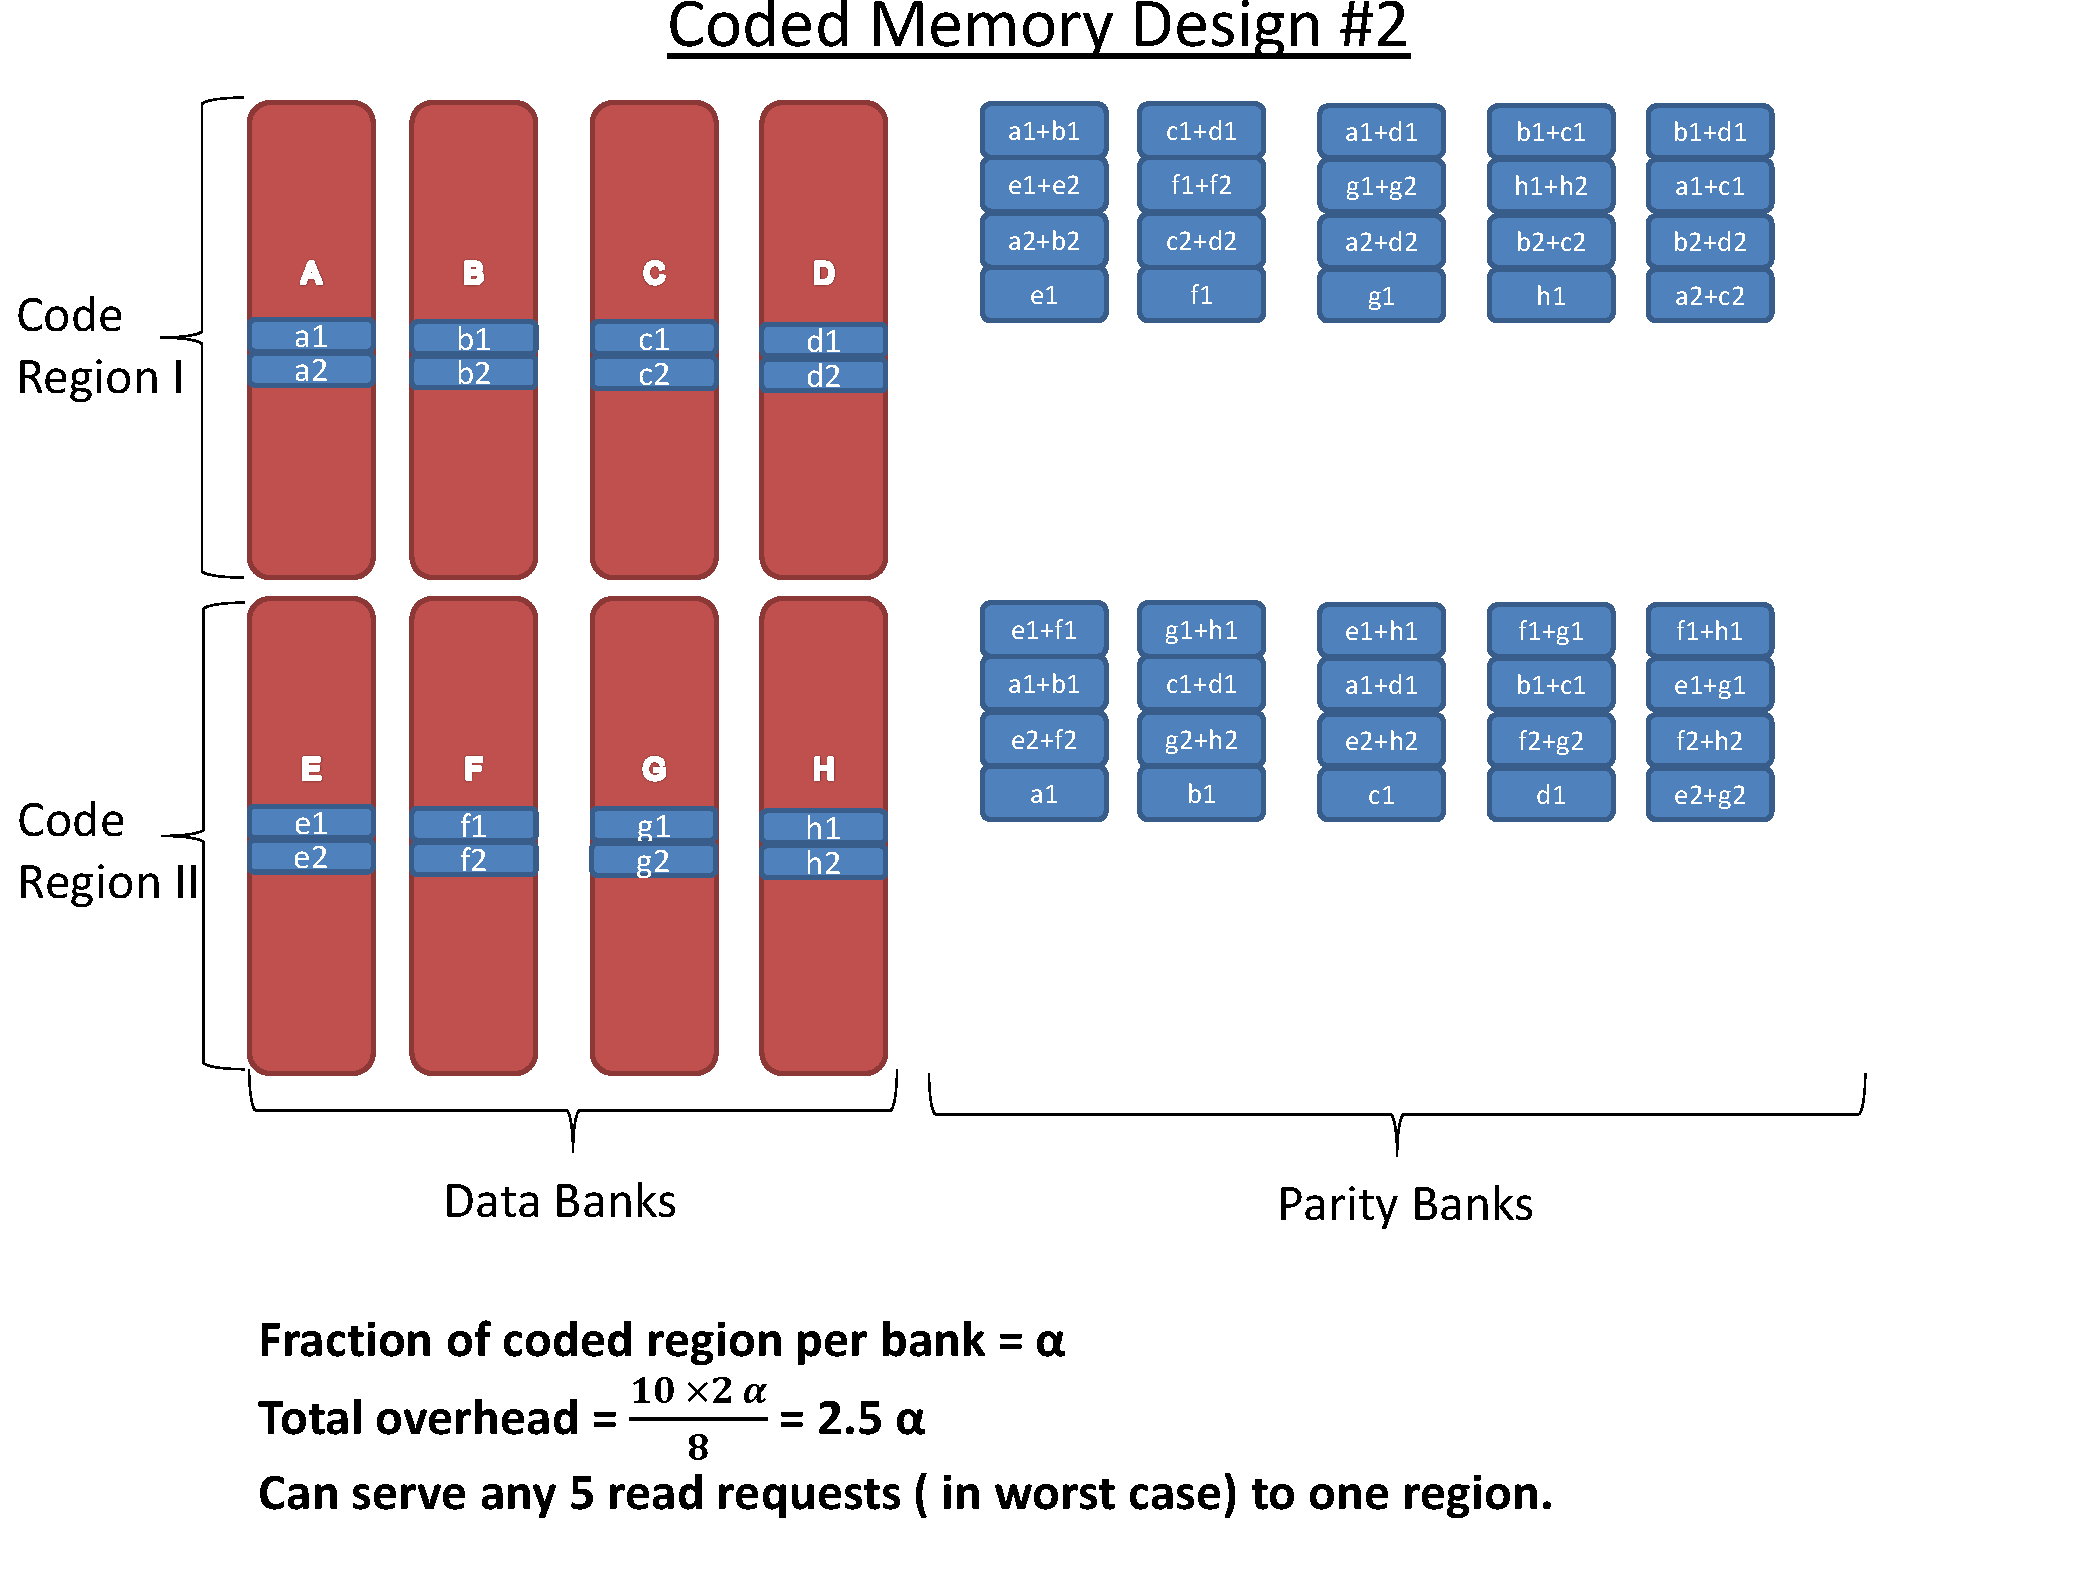
\includegraphics[width=1\linewidth]{fig/designII.pdf}
	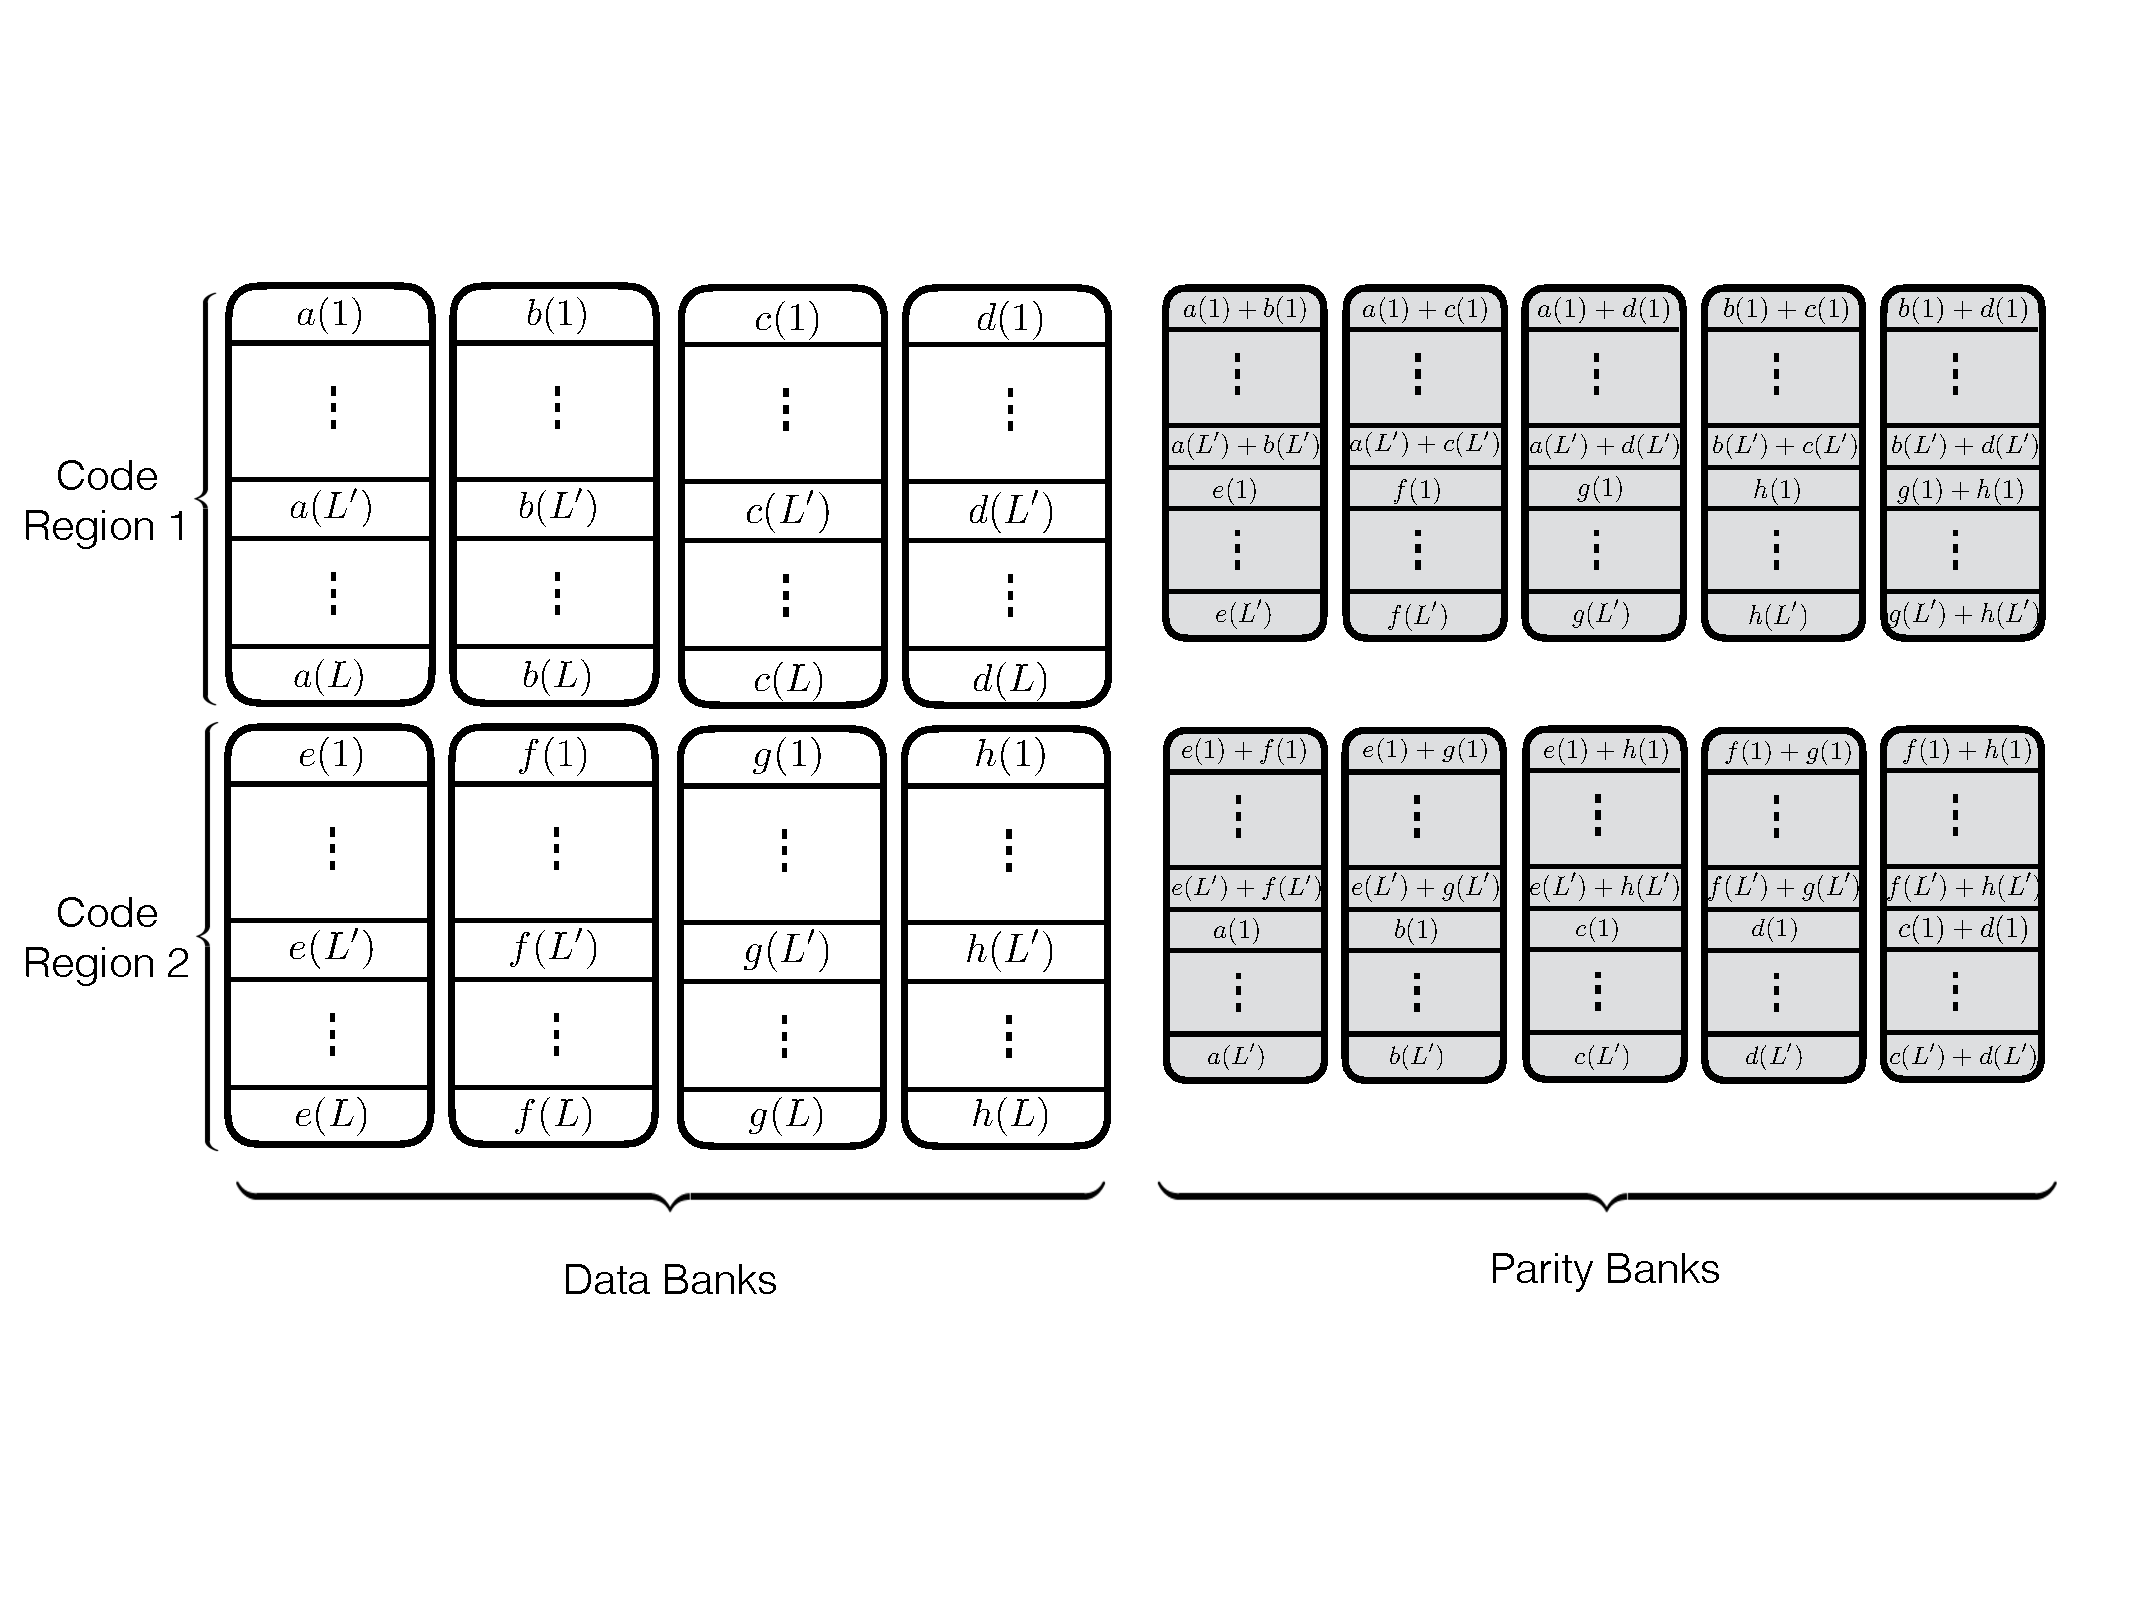
\includegraphics[width=1\linewidth]{fig/Code-Design-2.pdf}
	\caption{\it{Pictured here is an illustration of code scheme II.}}
	\label{fig:design2}
%\end{minipage}
\end{figure}

\noindent \textbf{Best case analysis:~} This code scheme achieves the best access performance when sequential accesses to the data banks are issued. In particular, this scheme can support up to $9$ read requests in a single memory clock cycle. Consider the scenario where we receive read requests for the following rows of the data banks. 
$$
\big\{a(1),b(1),c(1),d(1),a(2),b(2),c(2),d(2),a(3),b(3),c(3)\big\}
$$ Here, we can serve 
$\{a(1), b(1), c(1), d(1)\}$ using the data bank $\mathbf{a}$ with the parity banks storing the parity elements $\{a(1) + b(1),b(1)+c(1),c(1)+d(1)\}$. Similarly, we can serve the requests for the rows $\{a(2),b(2),d(2)\}$ using the data bank $\mathbf{b}$ with the parity banks storing the parity elements $\{a(2)+d(2), b(2)+d(2)\}$. Lastly, the request for the rows $c(2)$ and $d(3)$ is served using the data banks $\mathbf{c}$ and $\mathbf{d}$.\\


\noindent \textbf{Worst case analysis:~}The code scheme can enable $5$ simultaneous accesses in a single memory clock cycle in the
worst case. These are non-sequential and non-consecutive accesses to the memory banks. For 
example, when the access pattern corresponds to the rows $\{a(1),b(6),c(9),d(15),e(20)\}$, we can simultaneously serve 
these $5$ read requests with the help of our coded memory. In order to better utilize the unused banks in this case, we can use the prefetching 
mechanisms (cf. Section~\ref{sec:prefetching}) to look ahead in the queue and proactively download elements from the unused banks for future accesses.


% This design employs both inter-bank and intra-bank encoding in order to generate the content to be stored on the parity banks. In order to illustrate another flexibility that can be utilized while designing the storage space for a memory system, even though this code scheme encodes $\alpha L$ rows from each data bank, the parity banks are assumed to be storing $2\alpha L$ rows.


\subsubsection{Code Scheme III}
The next code scheme we discuss has locality 3, so each degraded read requires two parity banks to be served. This code scheme works with $9$ data bank $\{\mathbf{a}, \mathbf{b},\ldots, \mathbf{h}, \mathbf{z}\}$ and generates $9$ shallow parity banks. Figure~\ref{fig:design3} shows this scheme.
%The two designs discussed above achieve a rate of $2/5$. Here, we explore a code scheme which achieves a rate of $1/2$. 
%This design requires 9 data banks and 9 parity banks as shown in figure 5. It 
%also has a comparatively higher locality of 3. That is, it requires the memory 
%controller to "know" two out of three data elements to decode the third. 
The storage overhead of this scheme is $9\alpha L$ which corresponds to the rate of $\frac{1}{1 + \alpha}$. We note that this scheme possesses higher logical complexity as a result of its increased locality. 

This scheme supports $4$ simultaneous read access per bank per memory clock cycle as demonstrated by the following example. Suppose rows $\{a(1), a(2), a(3), a(4)\}$ are requested. $a(1)$ can be served directly from $\mathbf{a}$. $a(2)$ is served by means of a parity read and reads to banks $\mathbf{b}$ and $\mathbf{c}$, $a(3)$ is served by means of a parity read and reads to banks $\mathbf{d}$ and $\mathbf{g}$, and $a(4)$ is served by means of a parity read and reads to banks $\mathbf{e}$ and $\mathbf{z}$.

\noindent \textbf{Best case analysis:~} Following the analysis similar to Code Schemes I and II, the best case number of reads per cycle will be equal to the number of data and parity banks.

\noindent \textbf{Worst case analysis:~} Similar to coding schemes I and II, the number of reads per cycle is equal to the number of data banks. 
%The memory overhead here is less (just $\alpha$) compared to the previous designs. However, it possesses higher logical complexity because of increased locality. Example cases for this design are described below :
%\begin{itemize}
%
%	\item 4 reads for $a_0$: 1 read from $a_0$, 1 read from ($a_1$, $a_2$, 
%		$a_0$ + $a_1$ + $a_2$), 1 read from ($a_3$, $a_6$, $a_0$ + $a_3$ 
%		+ $a_6$), and the 4th read from ($a_4$, $a_8$, $a_0$ + $a_4$ + 
%		$a_8$).
%	\item 3 reads for $a_0$: 1 read from $a_0$, 1 read from ($a_3$, $a_6$, 
%		$a_0$ + $a_3$ + $a_6$), and the 3rd read from ($a_4$, $a_8$, 
%		$a_0$ + $a_4$ + $a_8$). \\
%	      1 read for $a_1$:  1 read from $a_1$.
%	\item 2 reads for $a_0$: 1 read from $a_0$ and the 2nd read from ($a_3$, 
%		$a_6$, $a_0$ + $a_3$ + $a_6$). \\
%	      2 reads for $a_1$: 1 read from $a_1$ and the 2nd read from ($a_4$, 
%	      $a_7$, $a_1$ + $a_4$ + $a_7$).
%	\item 2 reads for $a_0$: 1 read from $a_0$ and the 2nd read from ($a_3$, 
%		$a_6$, $a_0$ + $a_3$ + $a_6$). \\
%	      1 read for $a_1$: 1 read from $a_1$. \\
%	      1 read for $a_2$: 1 read from $a_2$.
%    \end{itemize}
%---------------------------------------
\begin{figure}[!ht]
	\centering
	\begin{minipage}[!t]{\linewidth}
		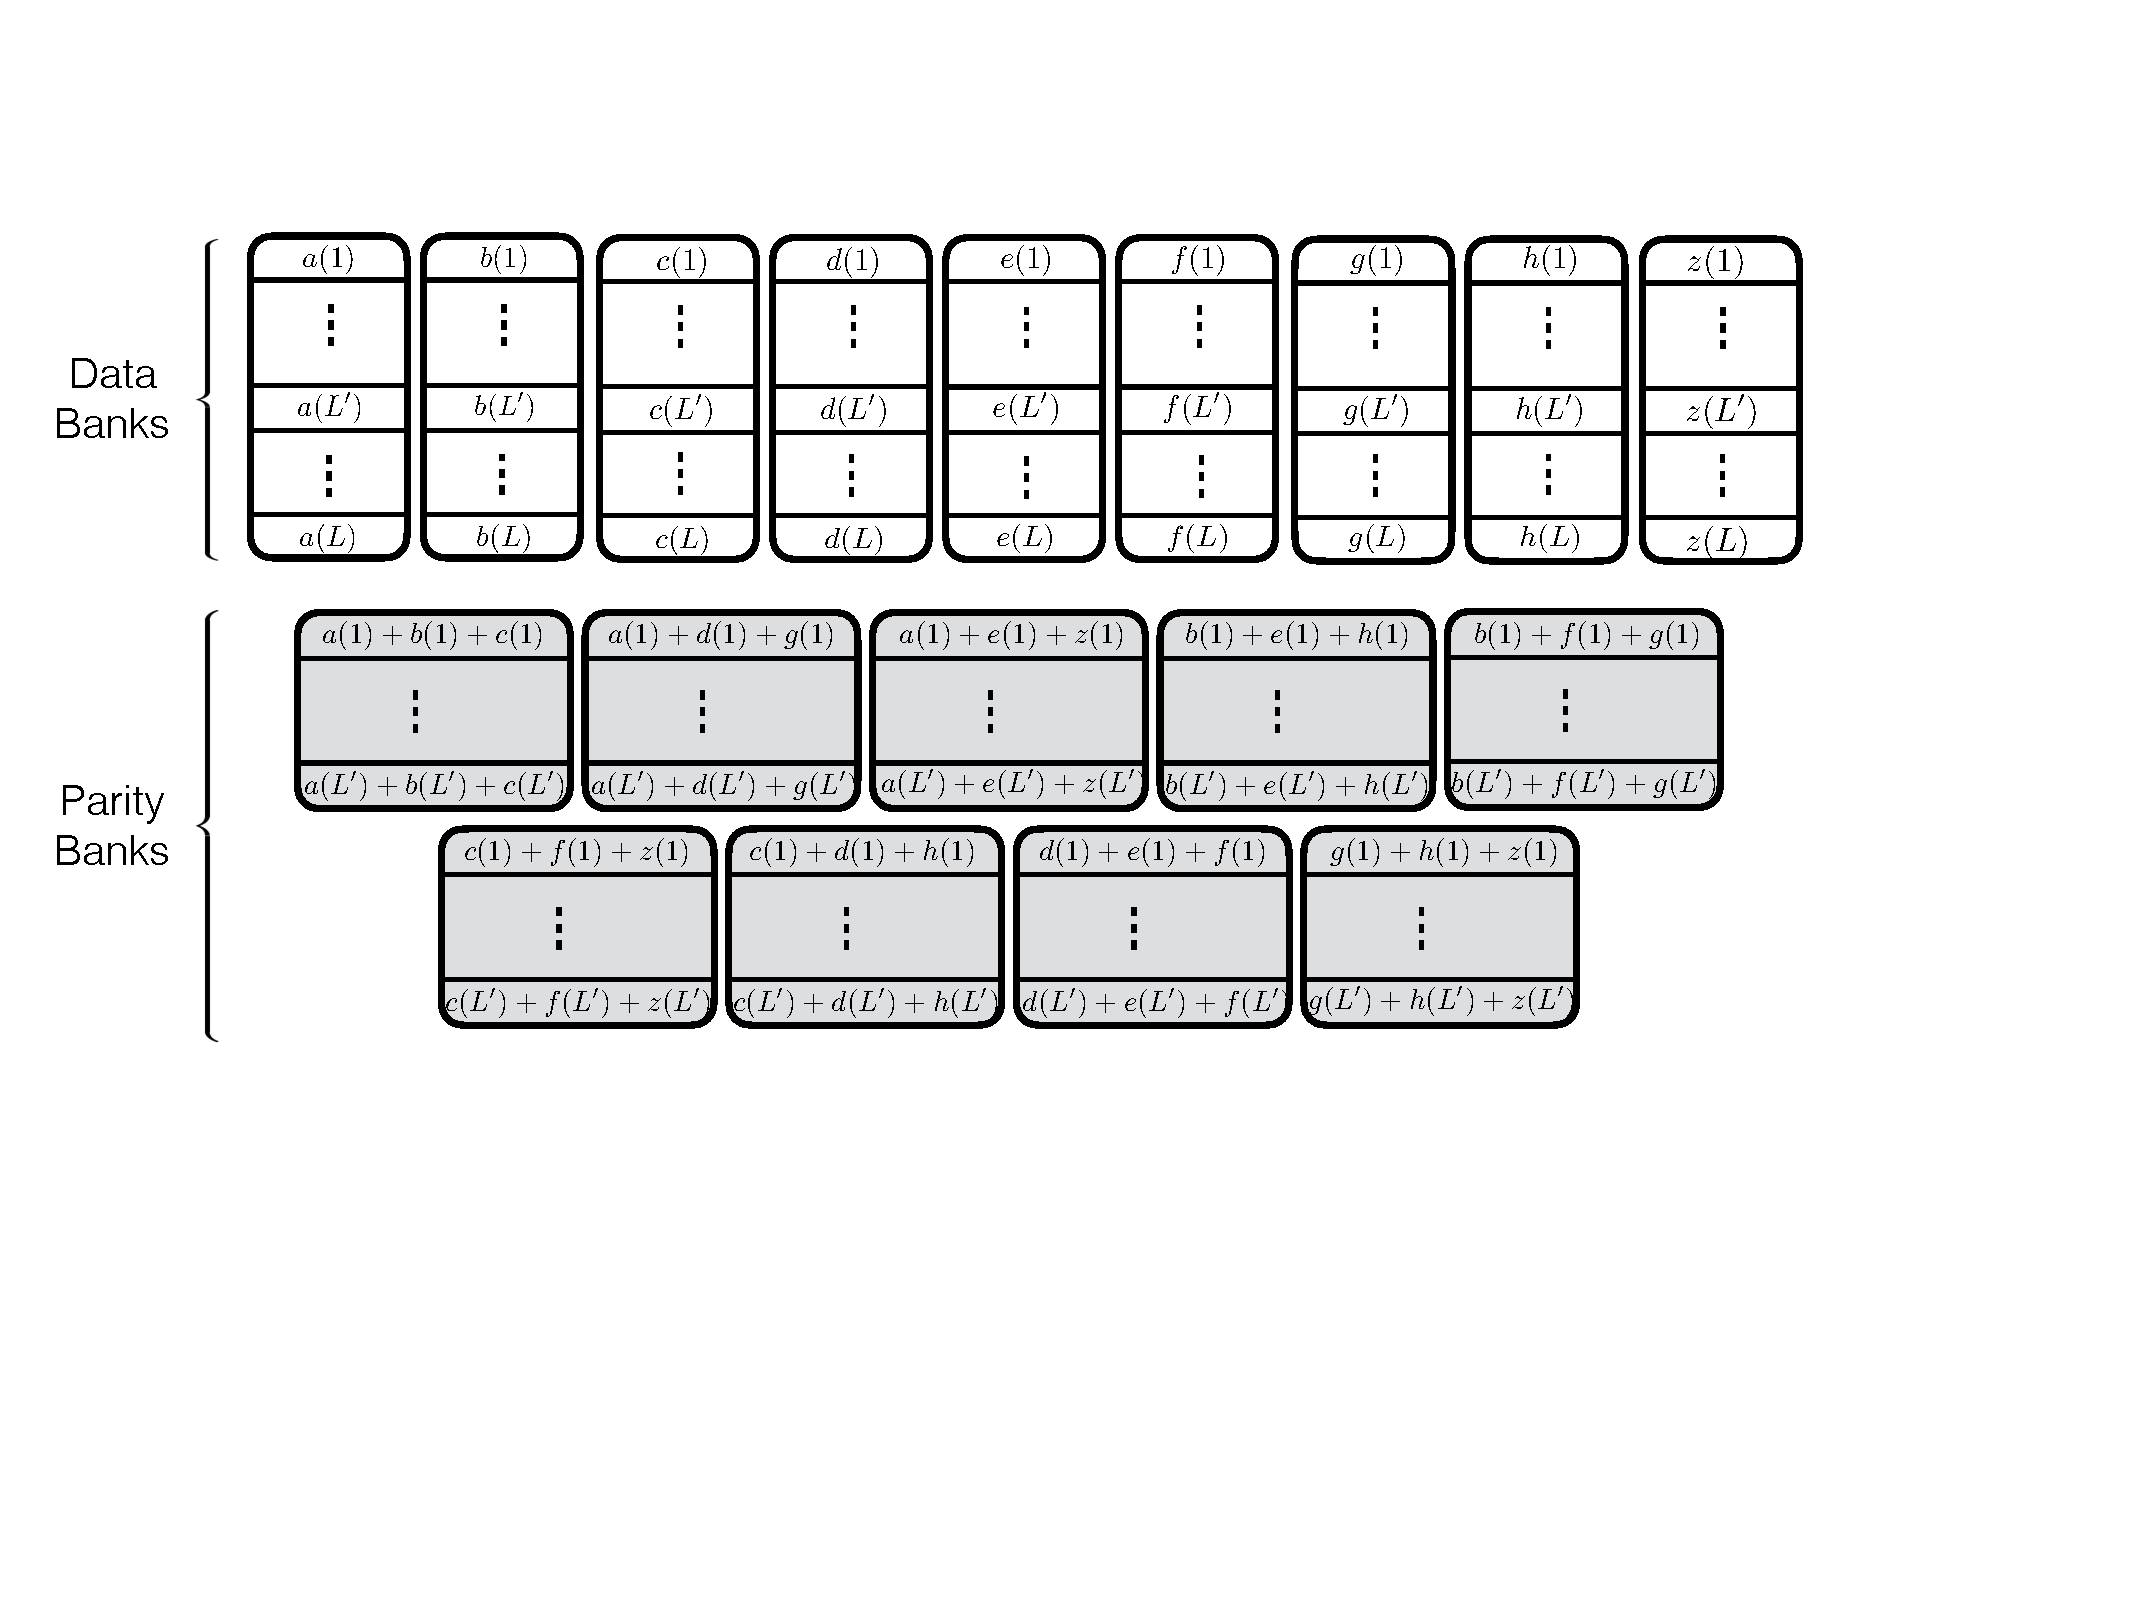
\includegraphics[width=\linewidth]{fig/Code-Design-3_9banks.pdf}
		\caption{\it{Pictured here is an illustration of code scheme III.}}
		\label{fig:design3}
	\end{minipage}
\end{figure}
%---------------------------------------

\begin{remark}
Note that the coding scheme in Figure~\ref{fig:design3} describes a system with $9$ data banks. However, we have set out to construct a memory system with $8$ data banks. It is straightforward to modify this code scheme to work with $8$ data banks $\{\mathbf{a}, \mathbf{b},\ldots, \mathbf{h}\}$ as shown in Figure~\ref{fig:design3_8}.
%Since most systems are implemented with number of banks as $2^n$ for some n. We present an 
%example of the code with 8 data banks in figure~\ref{fig:design3_8}. For using 8 data banks, 
%we drop the bank I. We also ignore the data from Bank I for constructing parity. So, three of 
%the parity banks have the locality of 2, while the rest of the parity banks have locality of 3.
% The new scheme for 8 data banks has 9 parity banks.
 \end{remark}
%---------------------------------------
\begin{figure}[!ht]
\centering
	\begin{minipage}[!t]{\linewidth}
		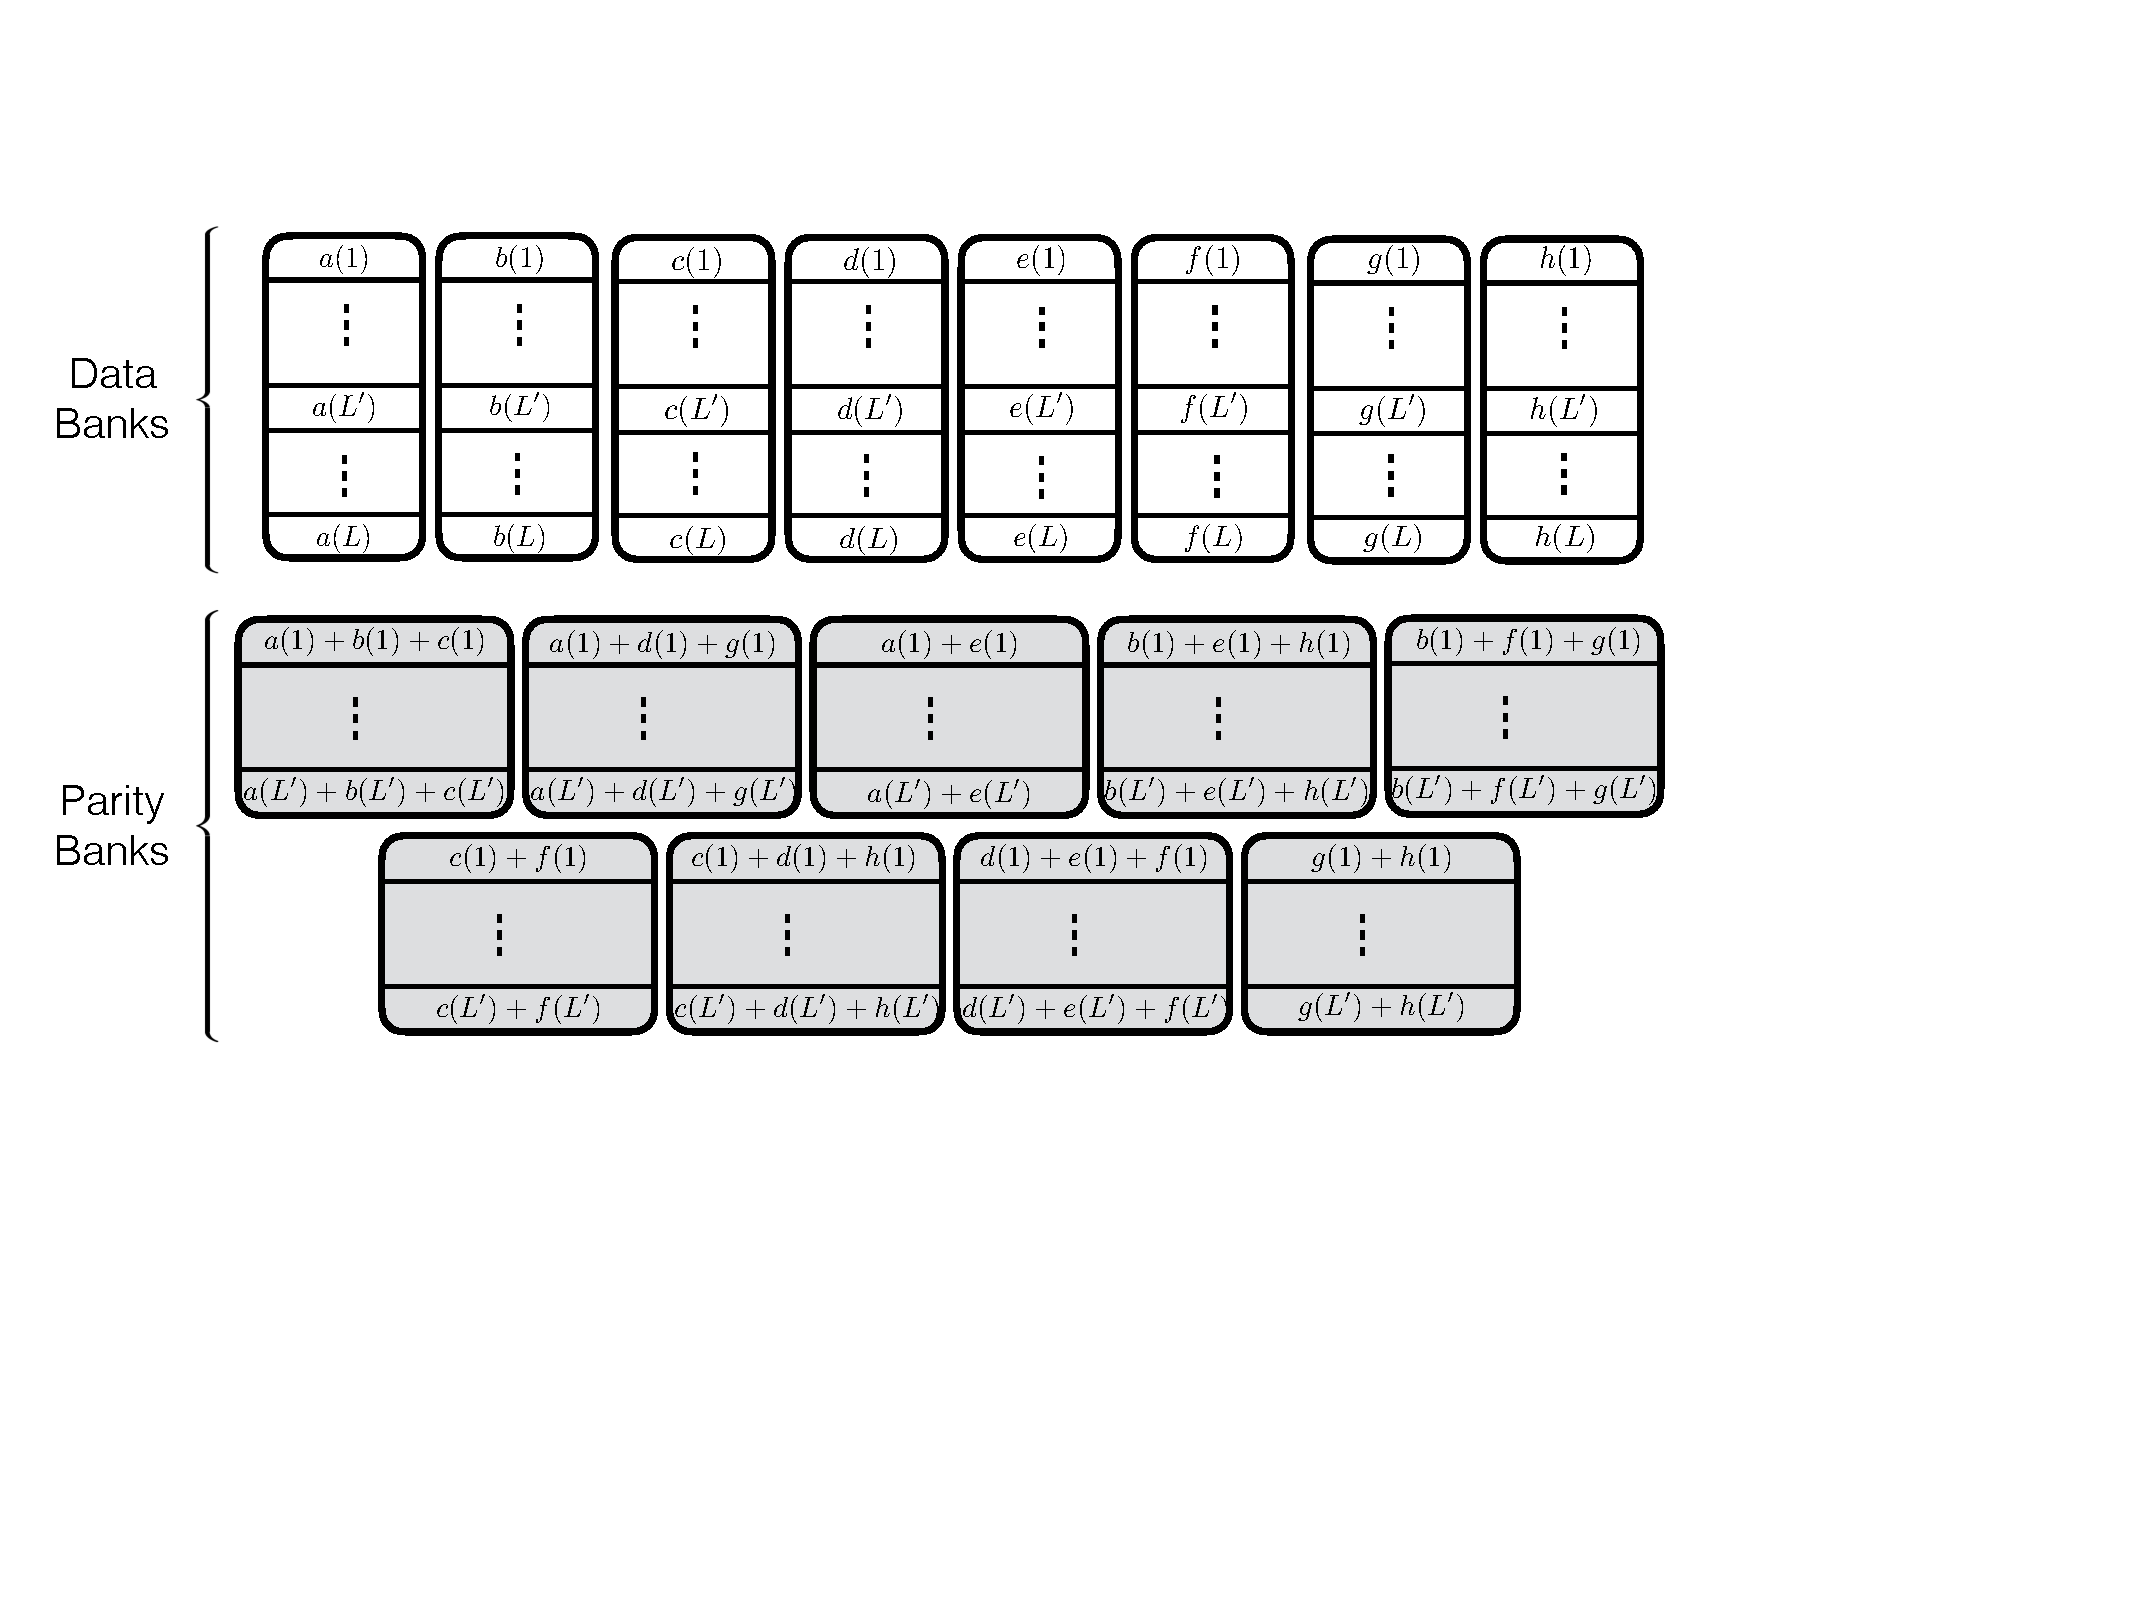
\includegraphics[width=\linewidth]{fig/Code-Design-3_8banks.pdf}
		\caption{\it{Pictured here is an illustration of code scheme III with 8 data banks.}}
		\label{fig:design3_8}
	\end{minipage}
\end{figure}
%---------------------------------------

\begin{comment}
Since the locality is 3 here in this design, i.e. , each parity is made up of combination of 3 data banks, we need to make sure that all three requests are in one line to be able to use the parity bank. 
For example parity bank 0 contains A+B+C. So, the following scenarios arise:
\begin{itemize}
	\item {\em Scenario I}: 1st request of A and 1st request of B are in same row. Then, we can search for a request in the same row for bank C by doing a look ahead. 
	\item {\em Scenario II}: 1st request of A and 1st request of C are in same row. Then, we can search for a request in the same row for bank B by doing a look ahead. 
	\item {\em Scenario III}: 1st request of B and 1st request of C are in same row. Then, we can search for a request in the same row for bank A by doing a look ahead. 
\end{itemize}
So, the simple pseudo code for doing this would be :\\
\begin{verbatim}
for each data bank 
    for each auxiliary bank1 of data bank
            Look ahead in auxiliary bank2 and check if 3 request in a row.
        end
    end
\end{verbatim}
Example: - \\
For {\bf data bank} to be {\bf A} \\
{\bf auxiliary bank1} goes from [B C D G A E] \\
{\bf auxiliary bank2} goes from [C B G D E A] \\
  The element A is just there in {\bf auxiliary bank1} and {\bf auxiliary bank2} to maintain the symmetry because A + E has locality of 2.
\end{comment}


%%%%%%%%%%%%%%%%%%%%%%%%%%%%%%%%%%%%%%%%%%%%%%%%%%%%%%%%
% Memory controller design
%%%%%%%%%%%%%%%%%%%%%%%%%%%%%%%%%%%%%%%%%%%%
\section{Memory Controller Design}
\label{sec:memcontrol}
%\Matt{BLUE: I would not mind removing this text. RED: I will likely remove this text}
The architecture of the memory controller is focused on exploiting redundant storage in the coding schemes to serve memory requests faster than an uncoded scheme.
%The memory design involves two key components: 1) storage space comprising of memory banks and 2) memory controller 
%The coding schemes discussed in previous section is implemented using systemC. 
%This section describes the architectural detail of how the schemes are 
%implemented using optimized algorithms. \\
%In this section, we explore the technique of dynamic coding in order to reduce 
%the memory and access overhead
%associated with the parity banks. We first discuss the scheme of dynamic coding 
%and follow it by discussing the potential benefits of prefetching the codes.\\
%\subsection{Memory Controller Stages}
%A general memory controller consists of three stages of processing illustrated in Figure~\ref{fig:multicore_arch}. The first stage, the {\em core arbiter}, receives memory access request from the master cores. The core arbiter then routes the requests to the proper {\em bank queue}. The bank queues are the second stage of processing, and they are responsible for storing and tracking memory requests. A memory request seeking memory located in bank $N$ will be sent to the $N$th bank queue. The {\em access scheduler} is the final stage of processing. It is responsible for scheduling the requests in the bank queues. Each memory cycle, the access scheduler generates an access pattern based on the requests present in the bank queues. The access pattern is a description of the reads or writes the memory controller will perform on the memory banks. Next, we discuss all of these three units and their functions in a greater detail.
%first level is {\em Core Arbiter }, the unit responsible for handling requests 
%from cores.  The second level is {\em Bank Arbiter} responsible for arbitrating 
%requests to banks.  The third level is {\em Access Scheduler} which schedules 
%most efficient access for each cycle.\\
% %%-----------------------
% \begin{figure}[htbp]
% \centering
% 	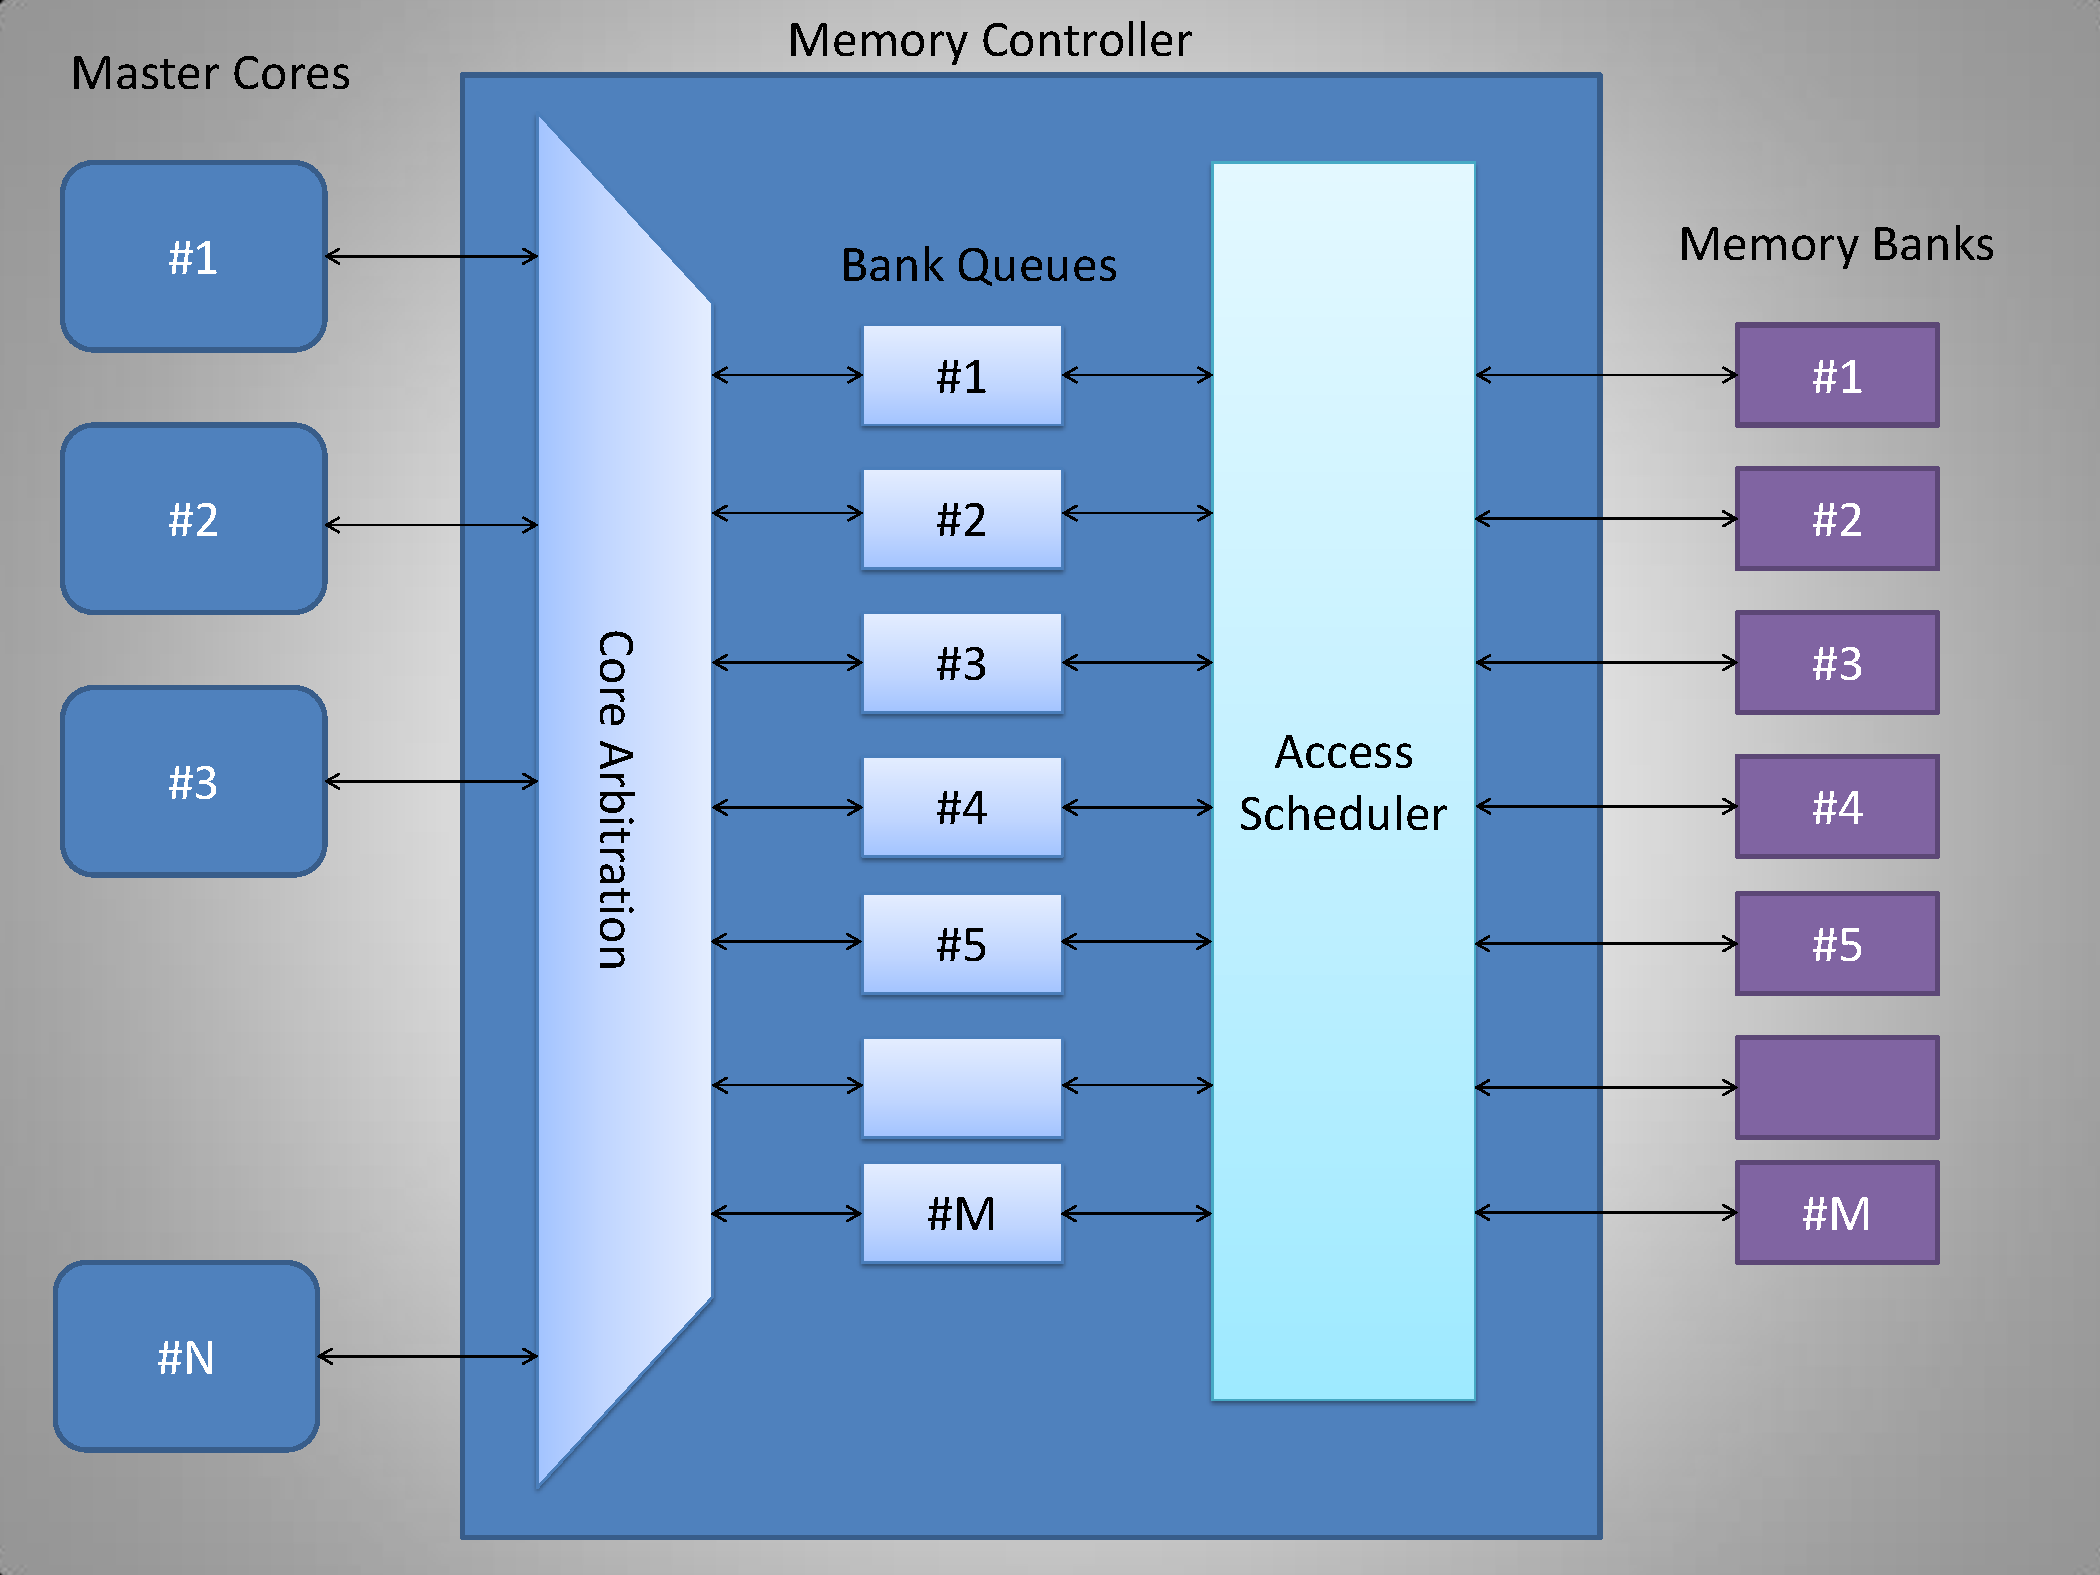
\includegraphics[width=0.7\linewidth]{fig/controllerArchitecture.pdf}
% \caption{
% {Architecture of Memory Controller} }
% \label{fig:pseudo-code}
% \end{figure}
% %-------------------------
The following three stages are illustrated in Figure~\ref{fig:multicore_arch}:
\begin{itemize}
\item \textbf{Core arbiter:~}Every clock cycle, the \textit{core arbiter} receives up to one request from each core which it stores in an internal queue. The core arbiter attempts to push these request to the appropriate bank queue. If it detects that the destination bank queue is full, the controller signals that the core is busy which stalls the core. The core arbiter also arranges the requests stored in its internal queue using a two-step priority order mechanism: first by Quality of Service (QoS) and then breaking ties with round-robin scheduling.

\item \textbf{Bank queues:~}Each data bank has a corresponding \textit{read queue} and \textit{write queue}.  The core arbiter sends memory requests to the bank queues until the queues are full. In our simulations, we use a bank queue depth of 10. There is also an additional queue which holds special requests such as memory refresh requests.

\item \textbf{Access scheduler:~}Every memory cycle, the \textit{access scheduler} chooses to serve read requests or write requests, algorithmically determining which requests in the bank queues it will schedule. The scheduling algorithms the access scheduler uses are called pattern builders. Depending on the current memory cycle's request type, the access scheduler invokes either the read or write pattern builder. A key design trade-off of the pattern builder algorithms is the relationship between the complexity of the algorithm and the number of requests the algorithm schedules.
\end{itemize}

We note that the core arbiter and bank queues should not differ much from those in a traditional uncoded memory controller. The access scheduler directly interacts with the memory banks, and therefore must be designed specifically for our coding schemes.


%-----------------------
\begin{figure}[tbp]
\centering
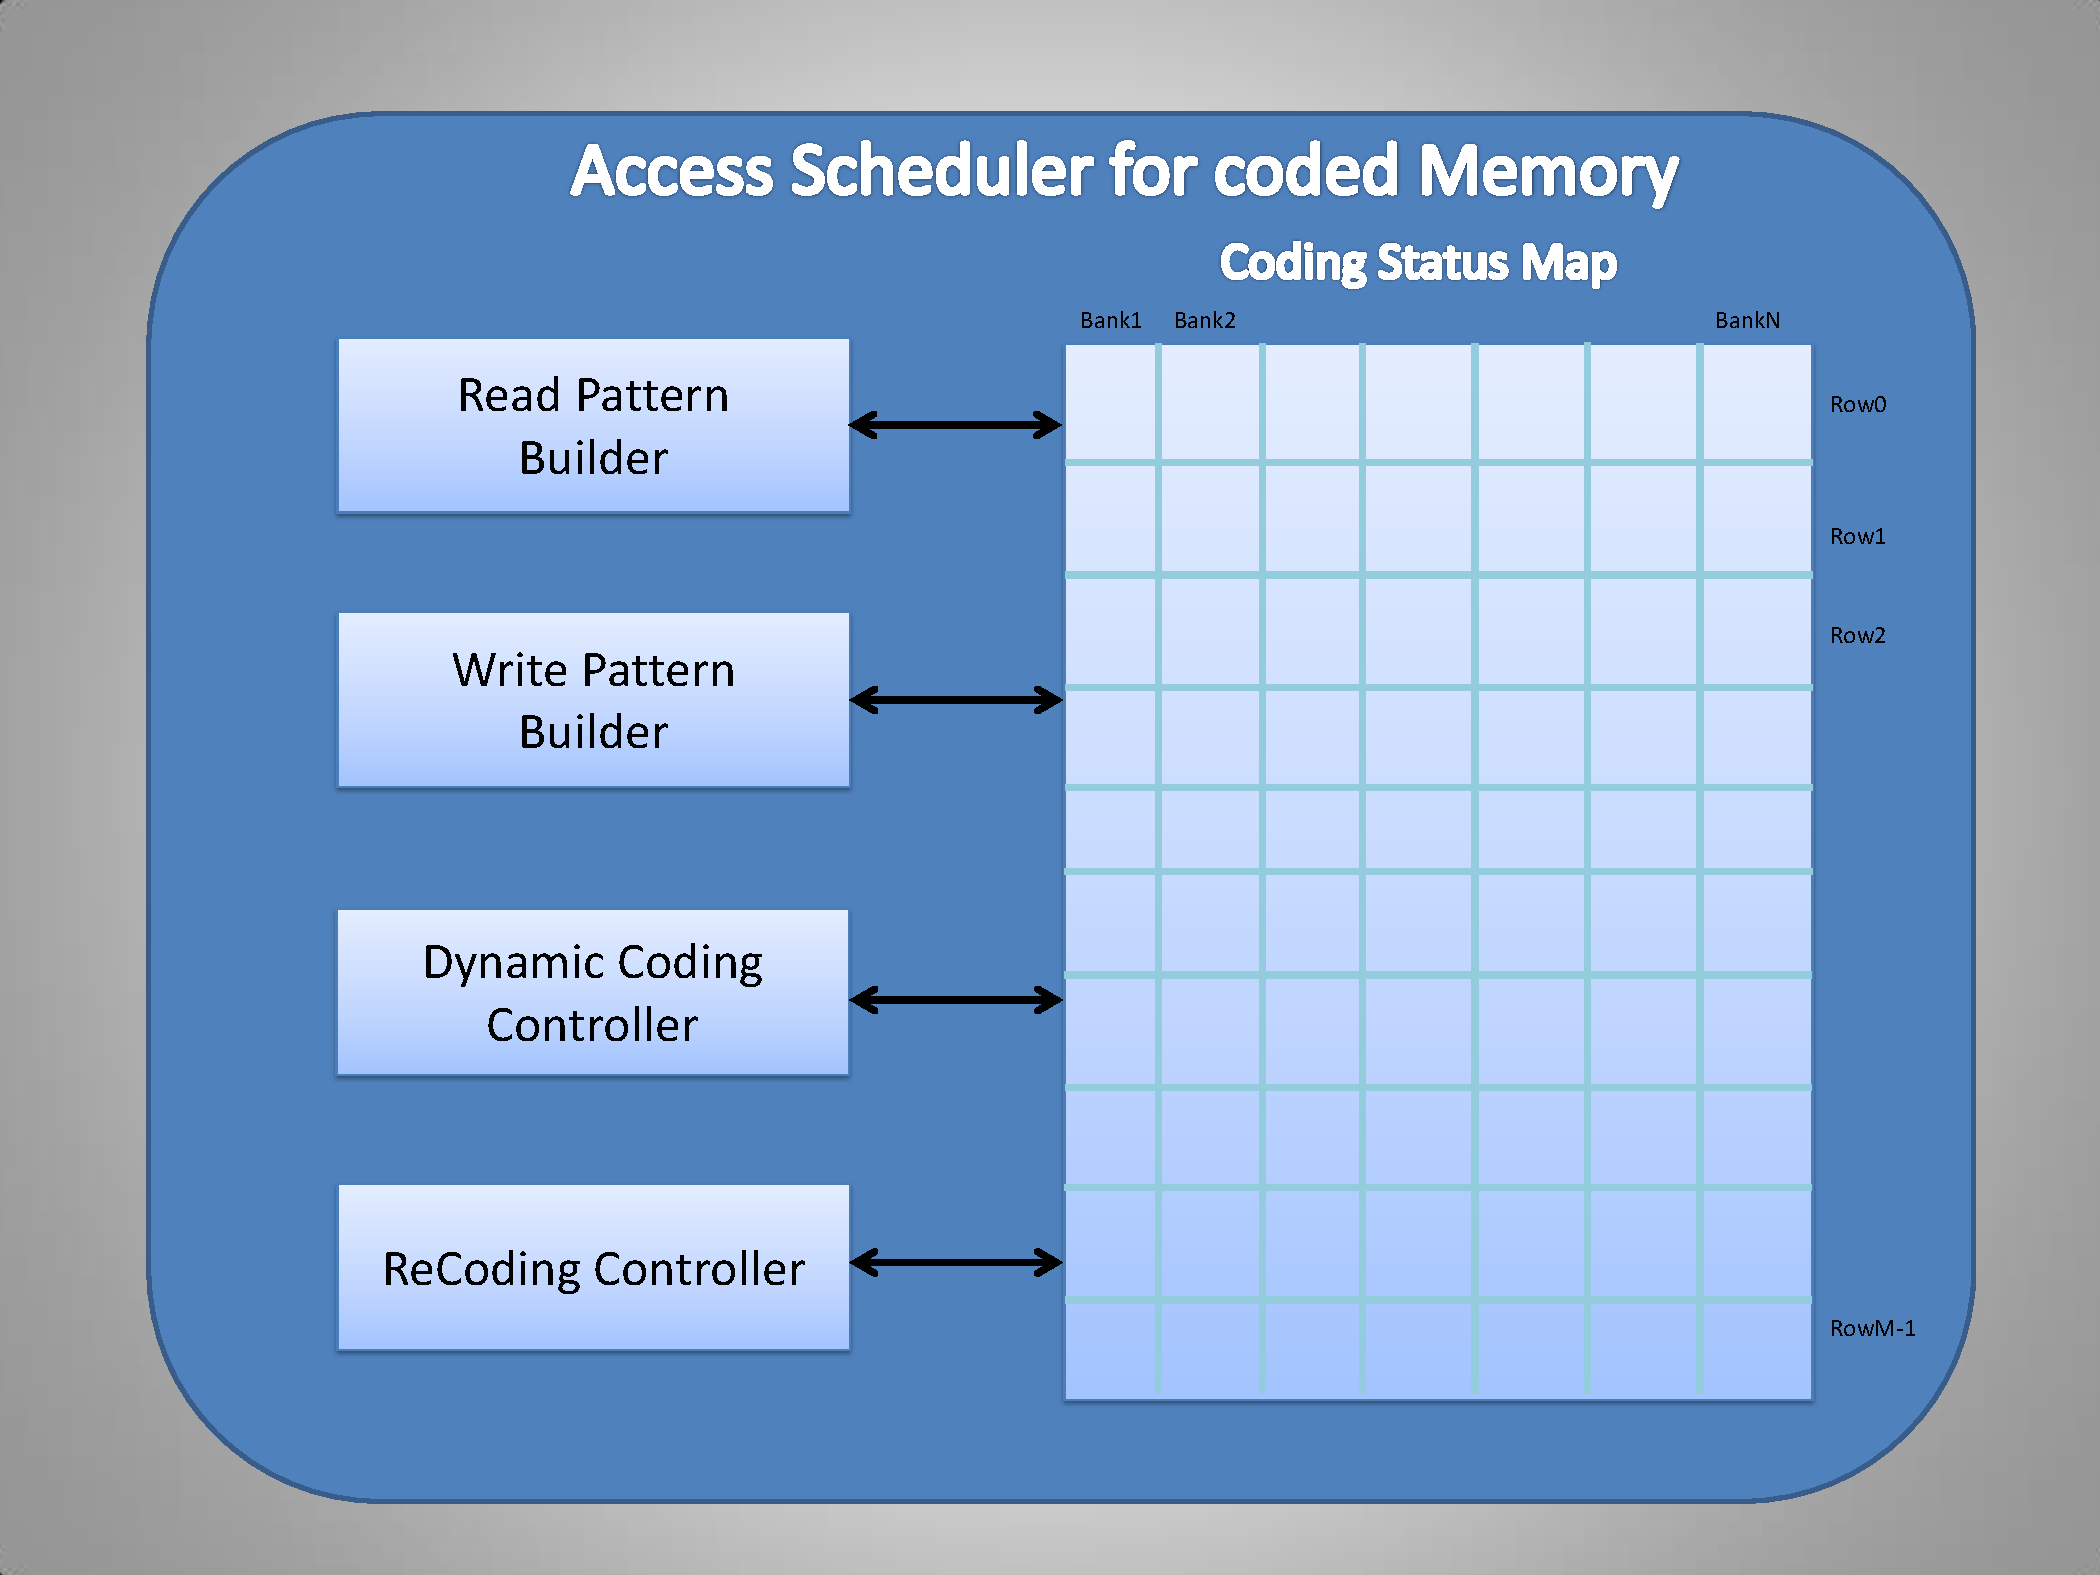
\includegraphics[width=0.7\linewidth]{fig/coded_access_scheduler.pdf}
\caption{
{Access scheduler for coded memory} }
\label{fig:coded_access_scheduler}
\end{figure}
%-------------------------
\subsection{Code Status Table}
\label{sec:codeStatusTable}
The code status table keeps track of the validity of data stored the data and parity banks. When a write is served to a row in a data bank, any parity bank which is constructed from the data bank will contain invalid data its corresponding row. Similarly, when the access scheduler serves a write to a parity bank, both the data bank which contains the memory address specified by the write request and any parity banks which utilizes that data bank will contain invalid data. The code status table keeps track of the locations of invalid data so the access scheduler does not erroneously serve read requests with stale data.

Figure~\ref{fig:coded_access_scheduler} depicts our implementation of the code status table. It contains an entry for every row in each data bank, which can take one of three values indicating 1) the data in both the data bank and parity banks is fresh, 2) the data bank contains the most recent data, or 3) one of the parity banks contains the most recent data. 
%It is not necessary for the code status table to know which parity bank a write request was served, because the dynamic coding unit described later in this section keeps track of this information. 
We assume that the elements of the code status table are accessible at a very fast rate. 


%{\color{red}
%This implementation of the code status table can be improved. This code status table does not keep track of the intermediate steps the access scheduler takes when rebuilding codes after a write is served. When rebuilding the memory in two parity banks after a data bank has been written to, it is likely that elements of one parity bank will be restored before the other. The restored parity bank is ready to serve more memory requests using the rebuilt row, but the code status table will indicate that all the parity banks are unavailable until all parity banks are restored. Full knowledge of the status of all data and parity banks allows the access scheduler to serve more requests in some scenarios. \Matt{is this example necessary? Is the tangent worth the insight?}
%}

%-----------------------
\begin{figure}[t!]
	%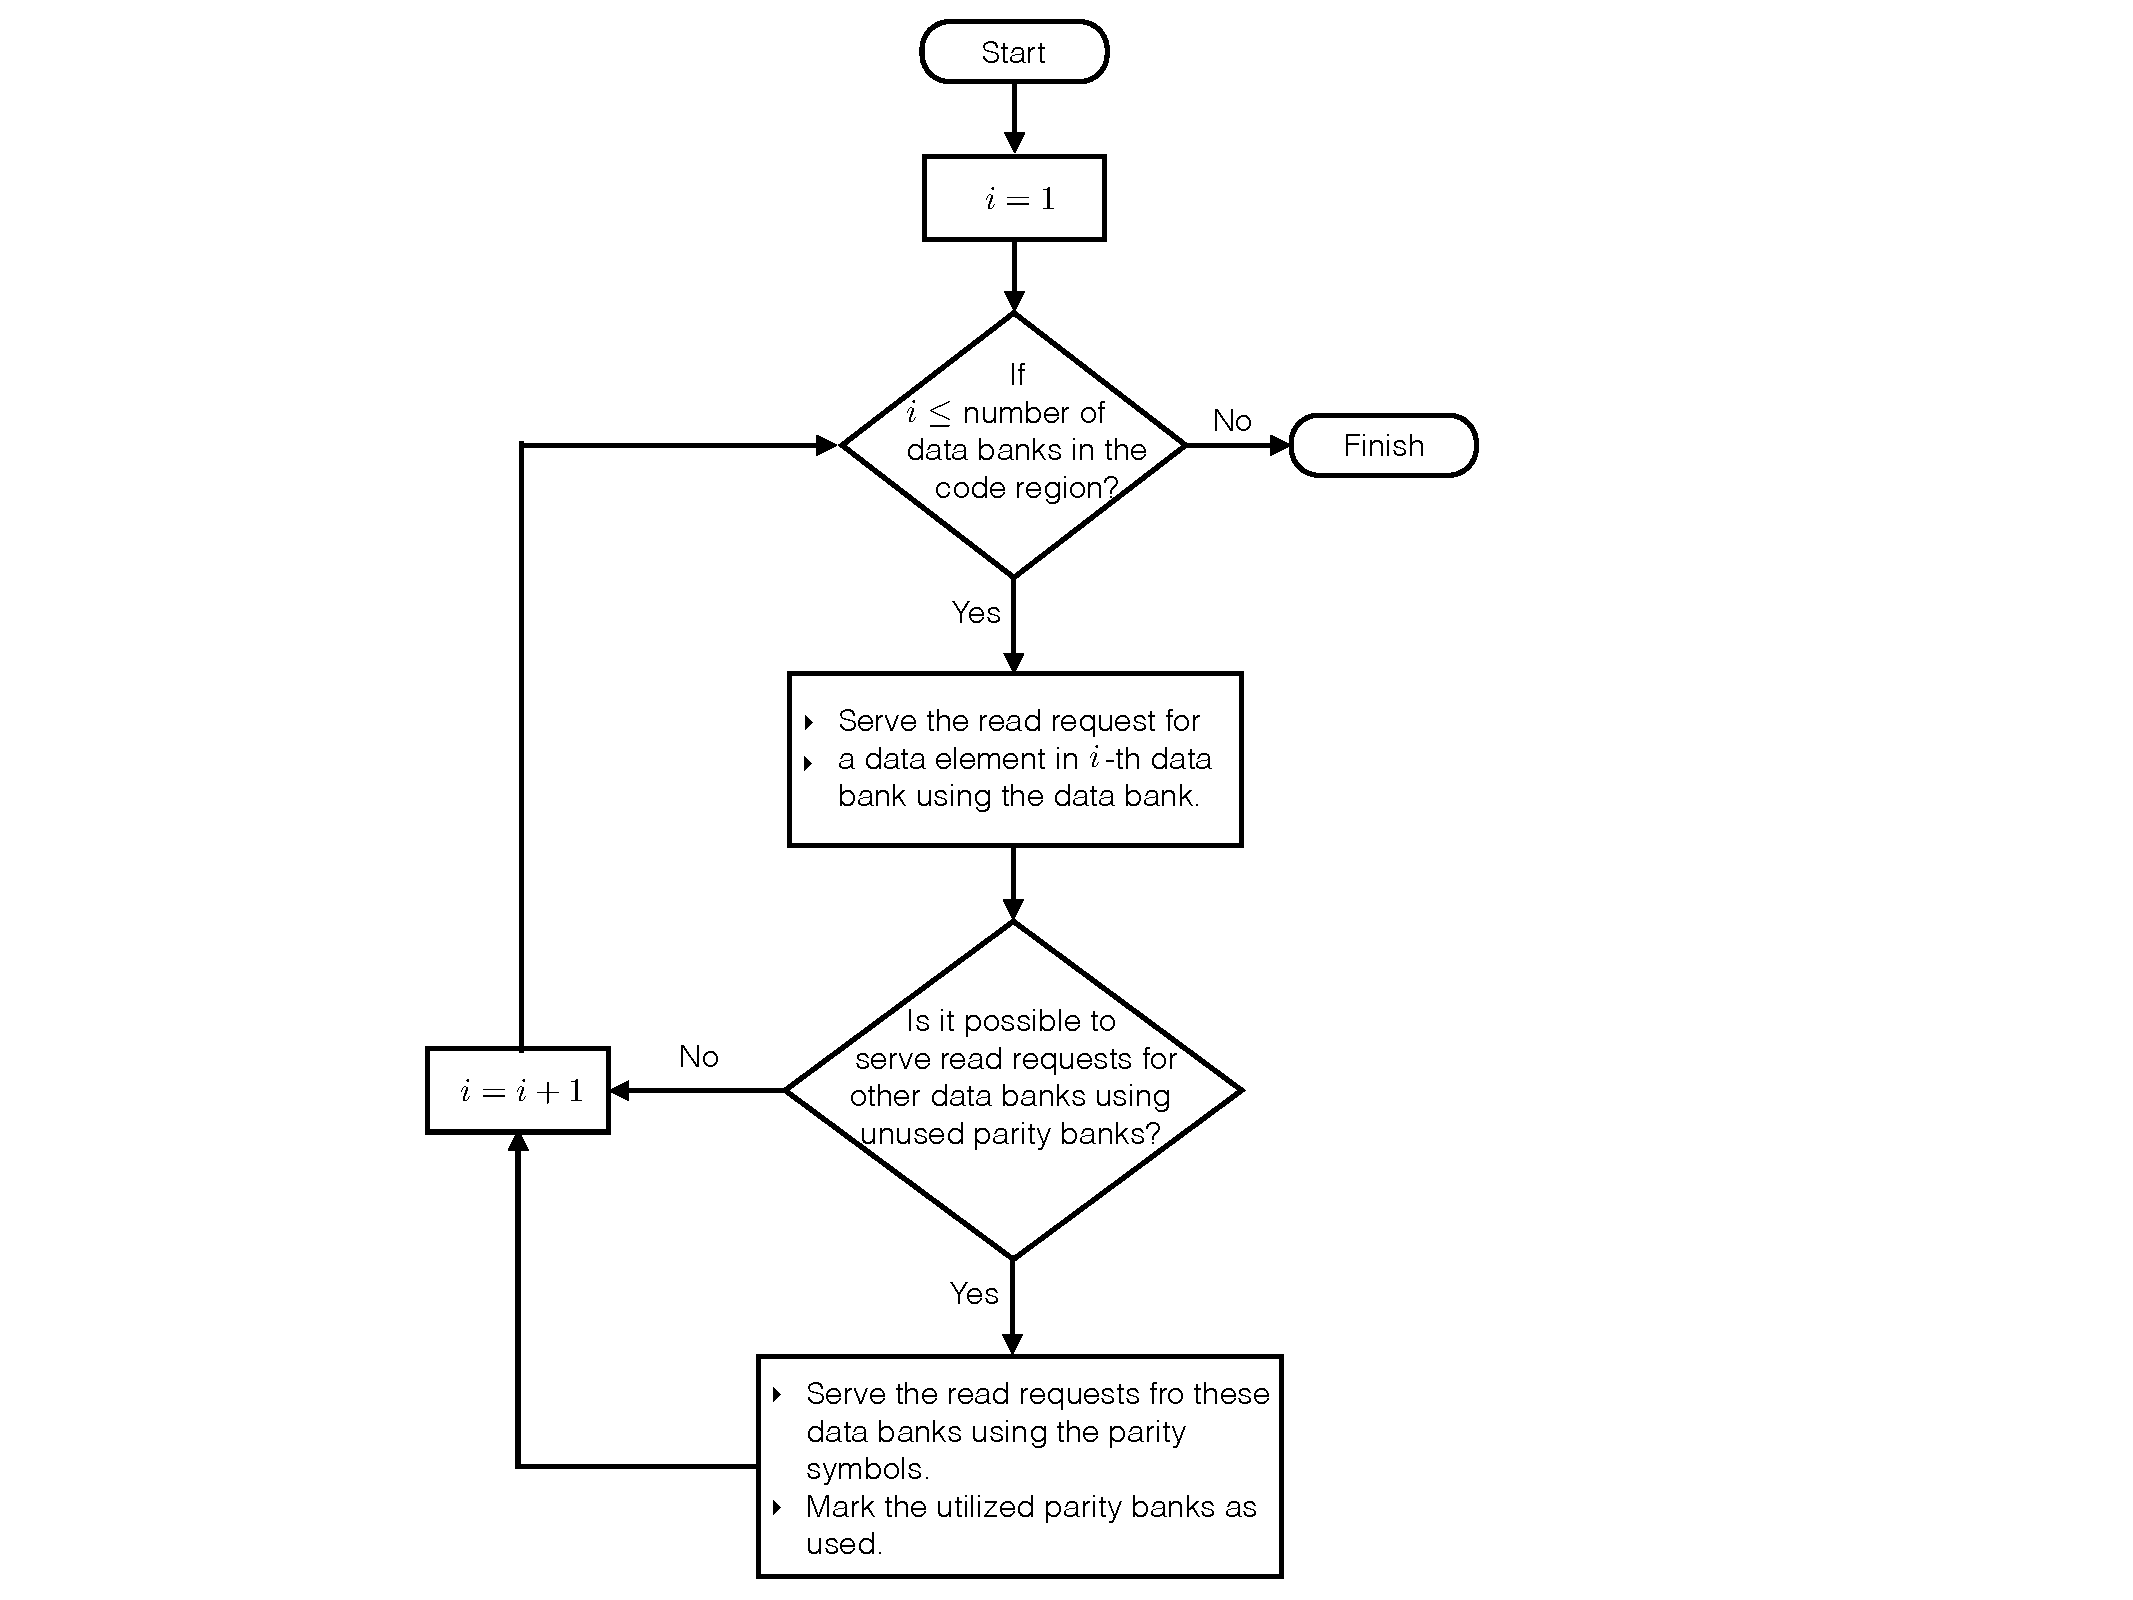
\includegraphics[width=0.9\linewidth]{fig/Read-algo.pdf}
	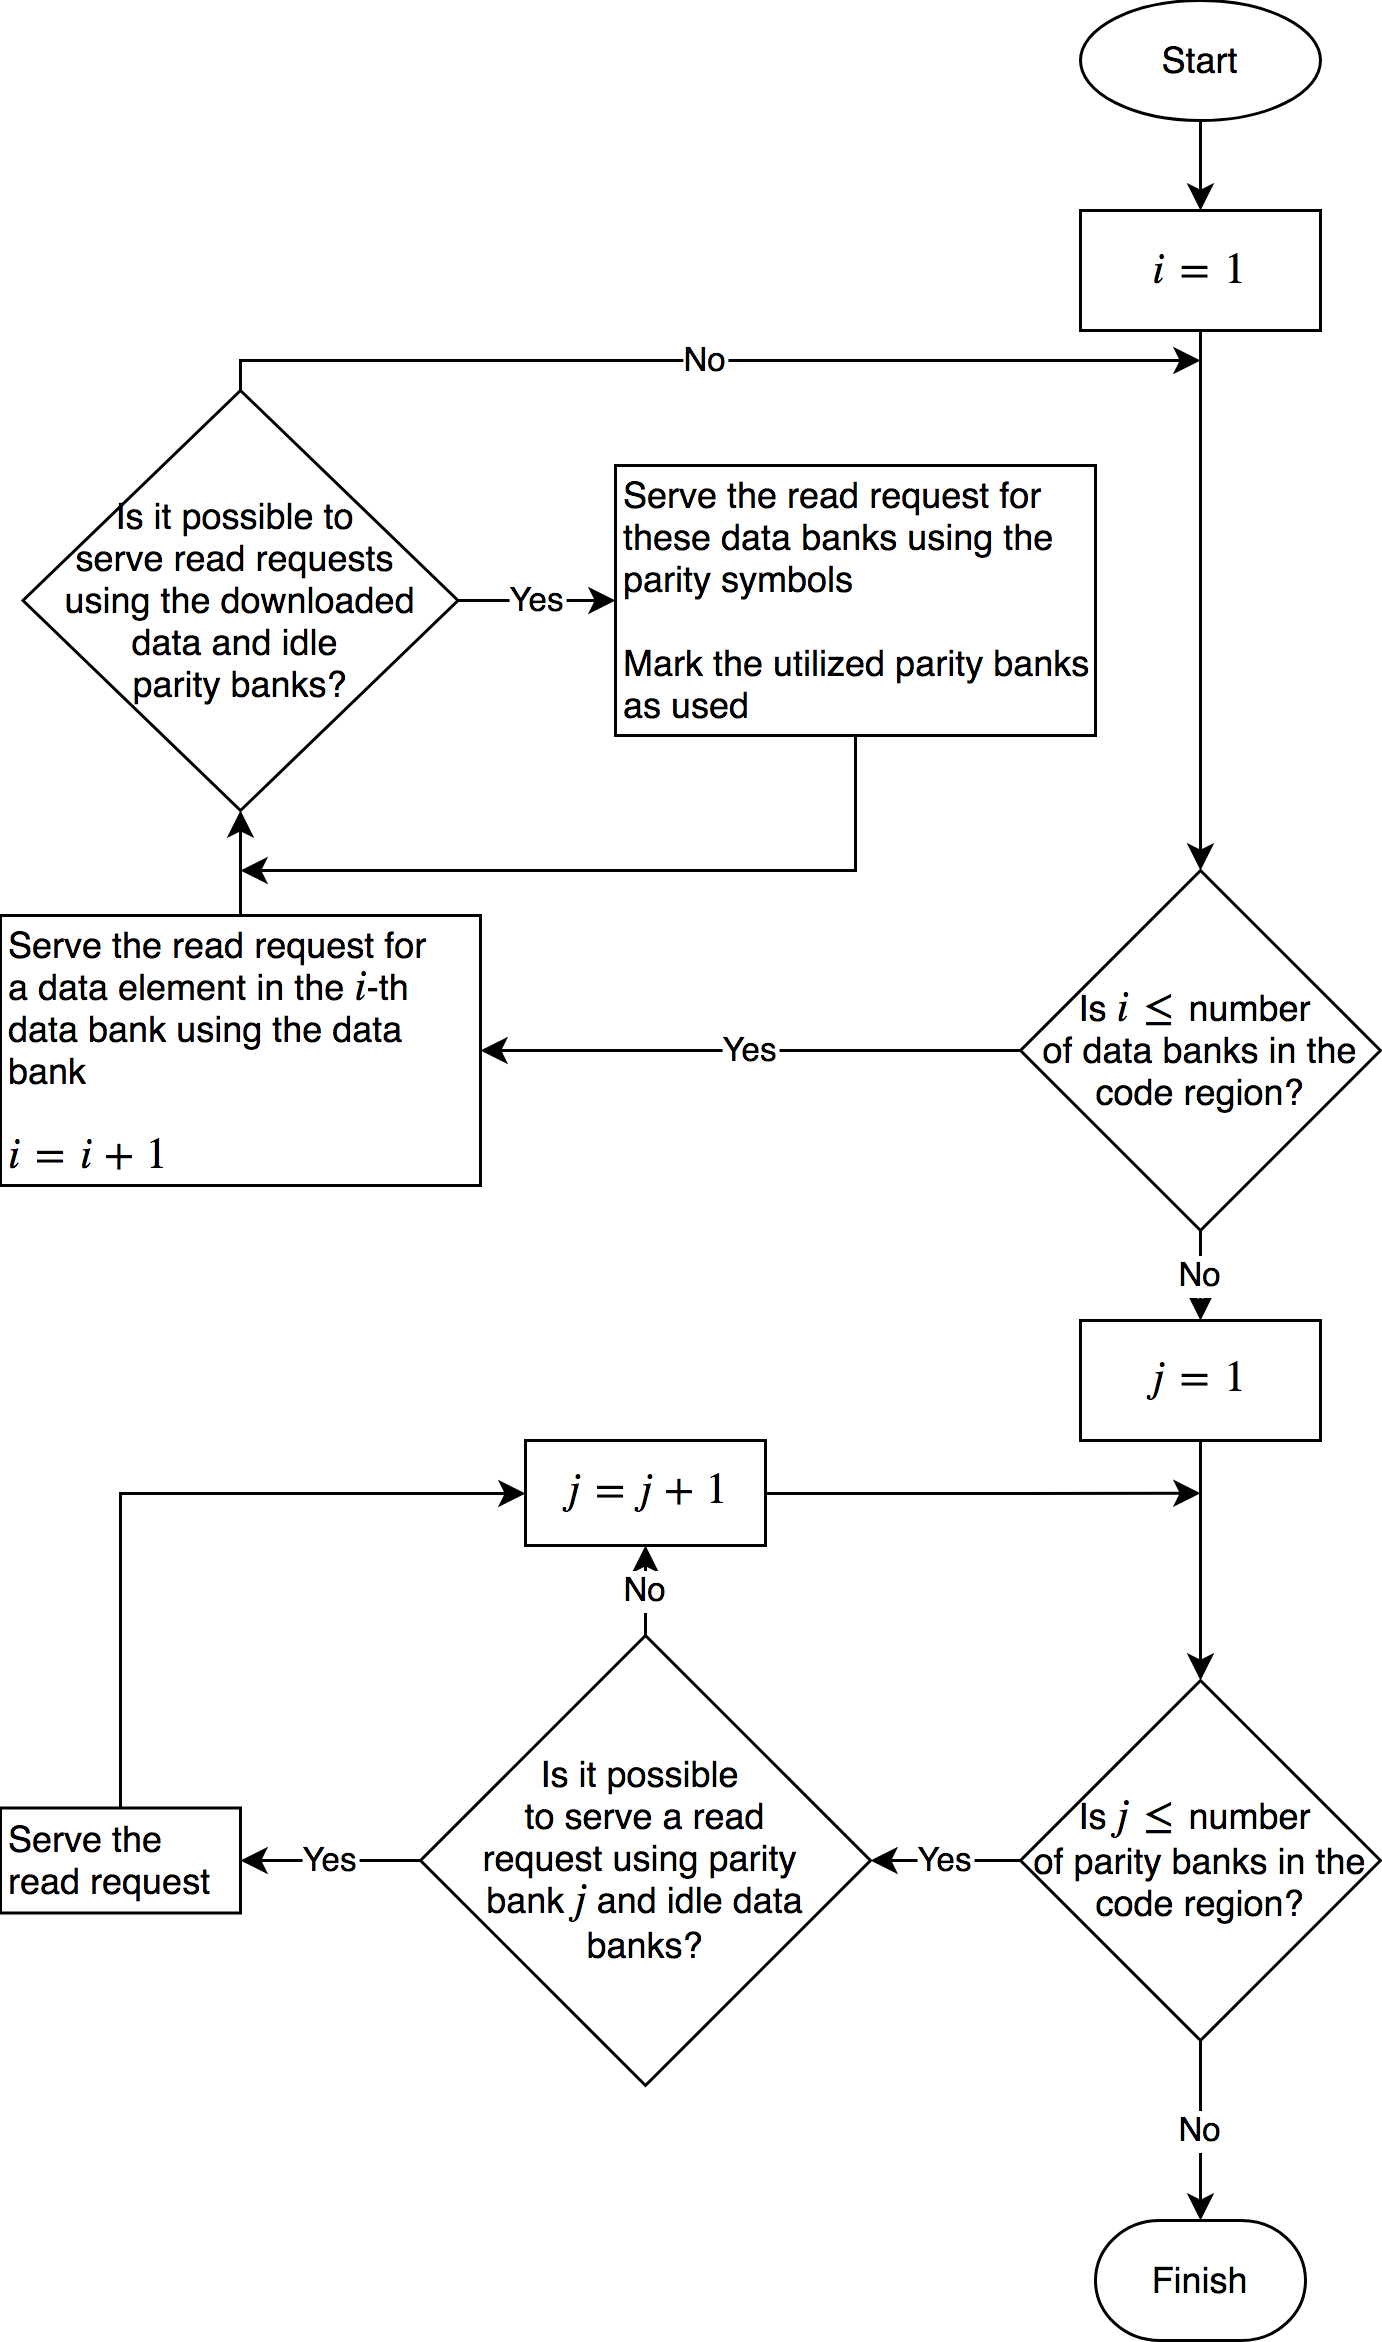
\includegraphics[width=0.96\linewidth]{fig/read_pattern_algo.png}
	\caption{{Description of the algorithm to build a read request pattern to be served in a given memory cycle.}}
	\label{fig:readAlgo}
\end{figure}
%-------------------------
%-----------------------
\begin{figure}[htbp]
	\centering
	%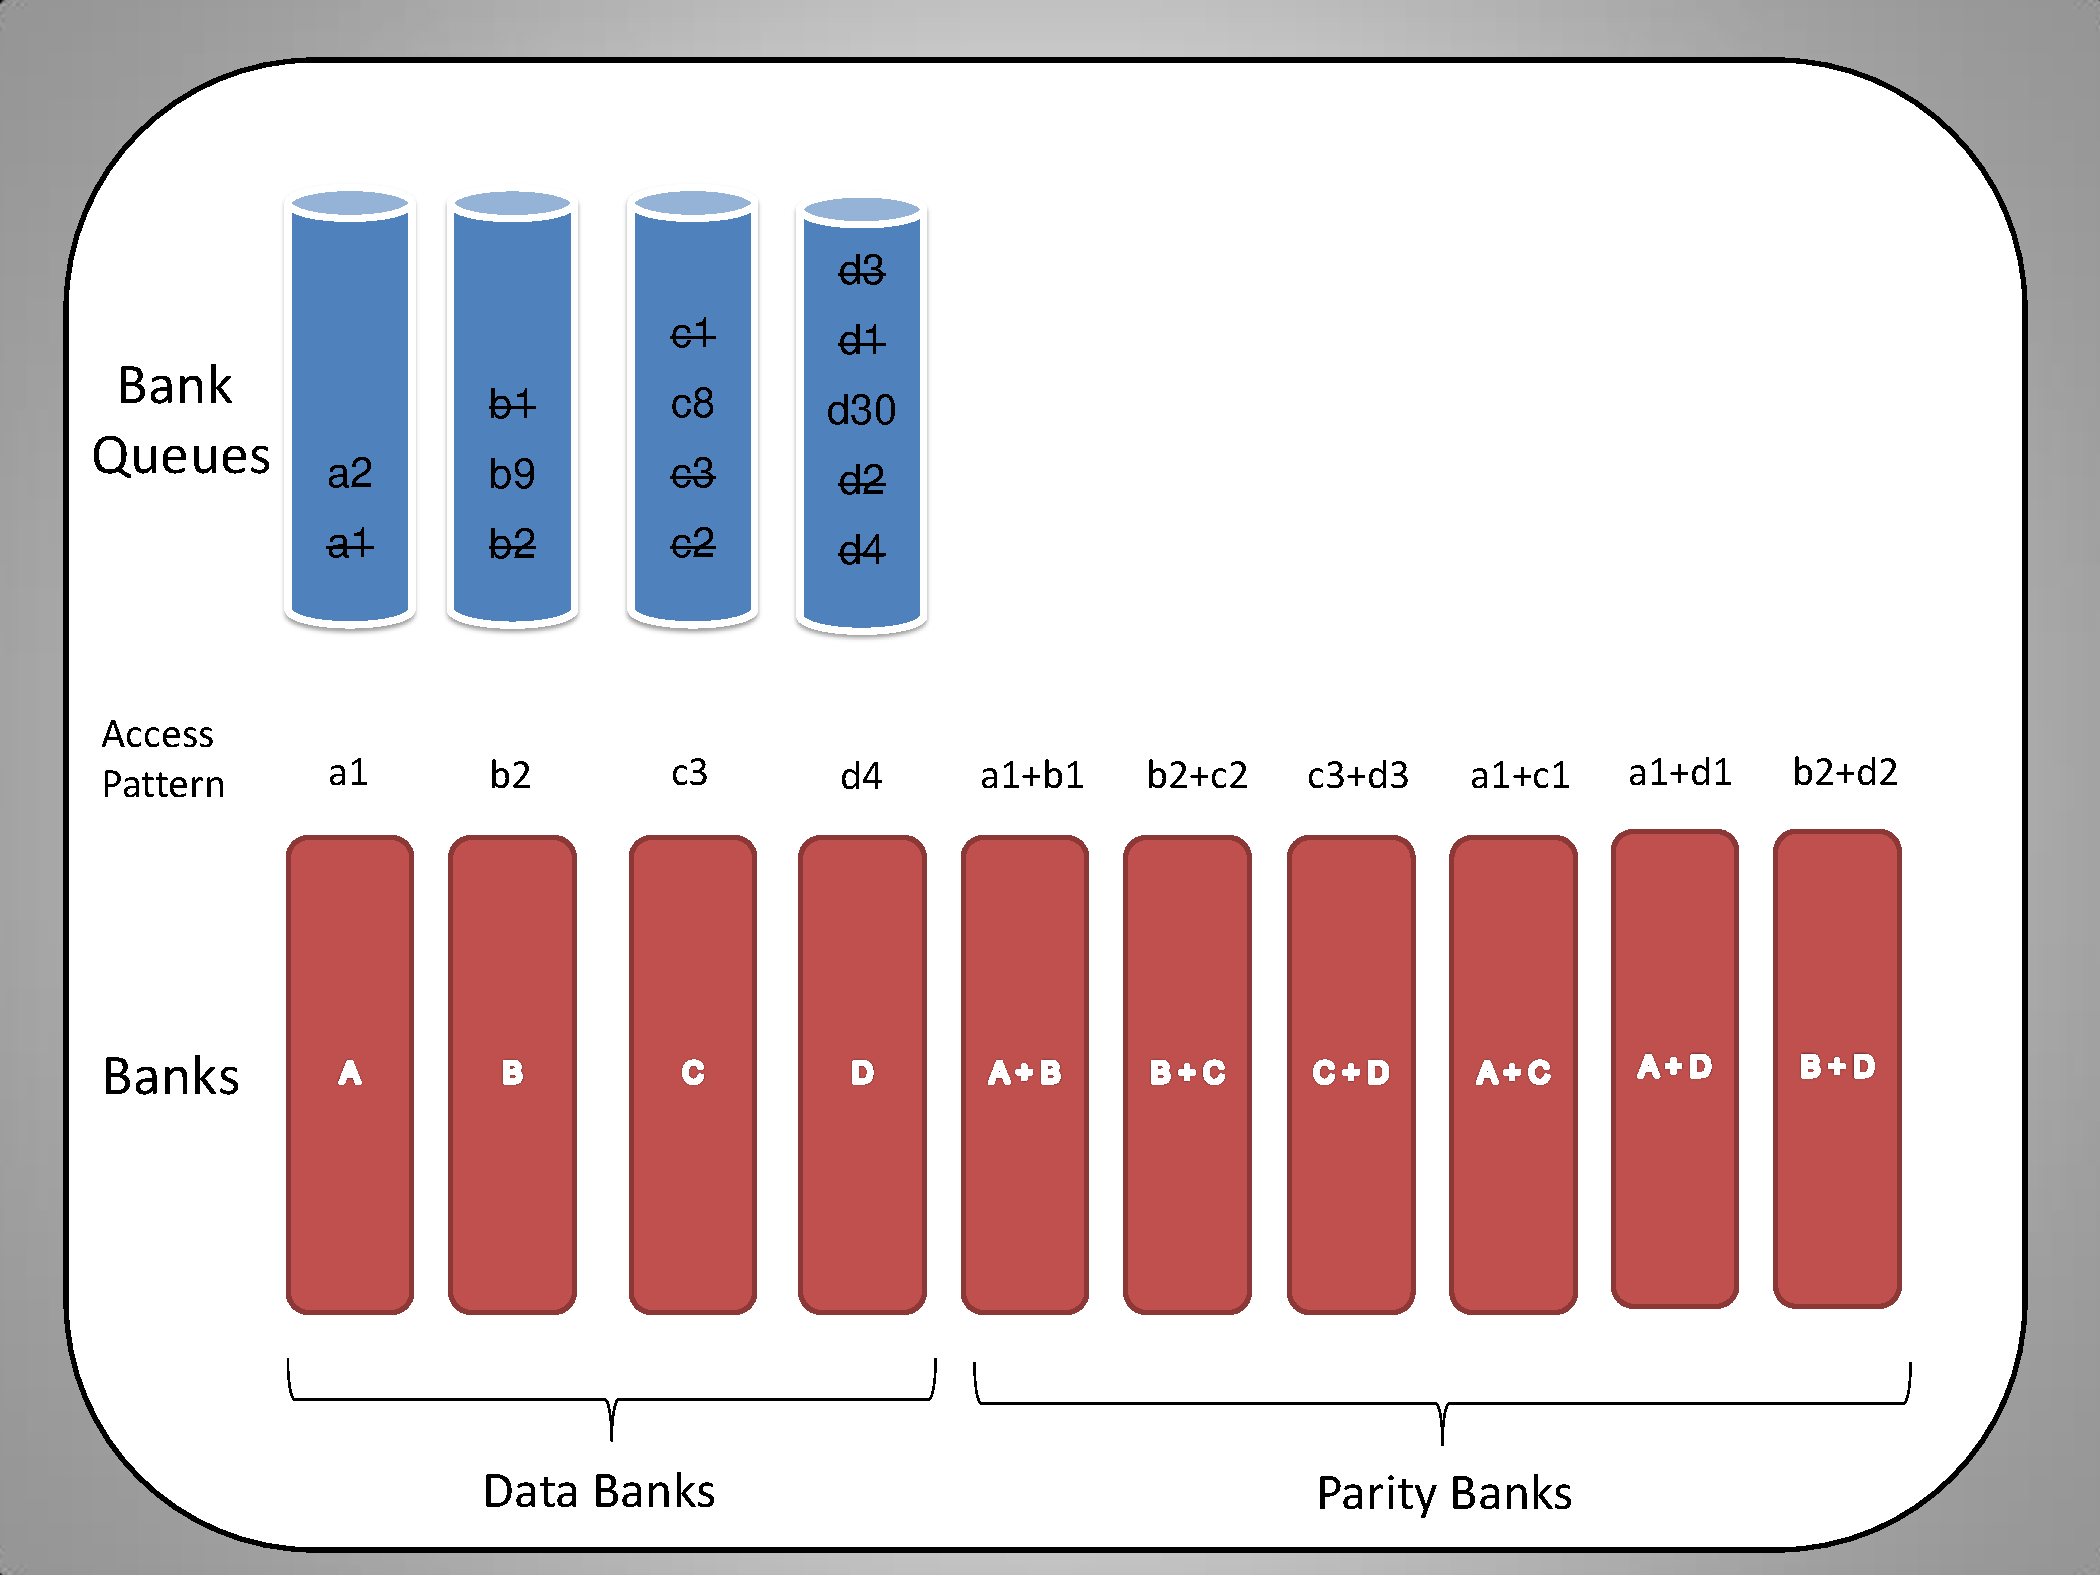
\includegraphics[width=0.7\linewidth]{fig/readAlgoAccessPattern.pdf}
	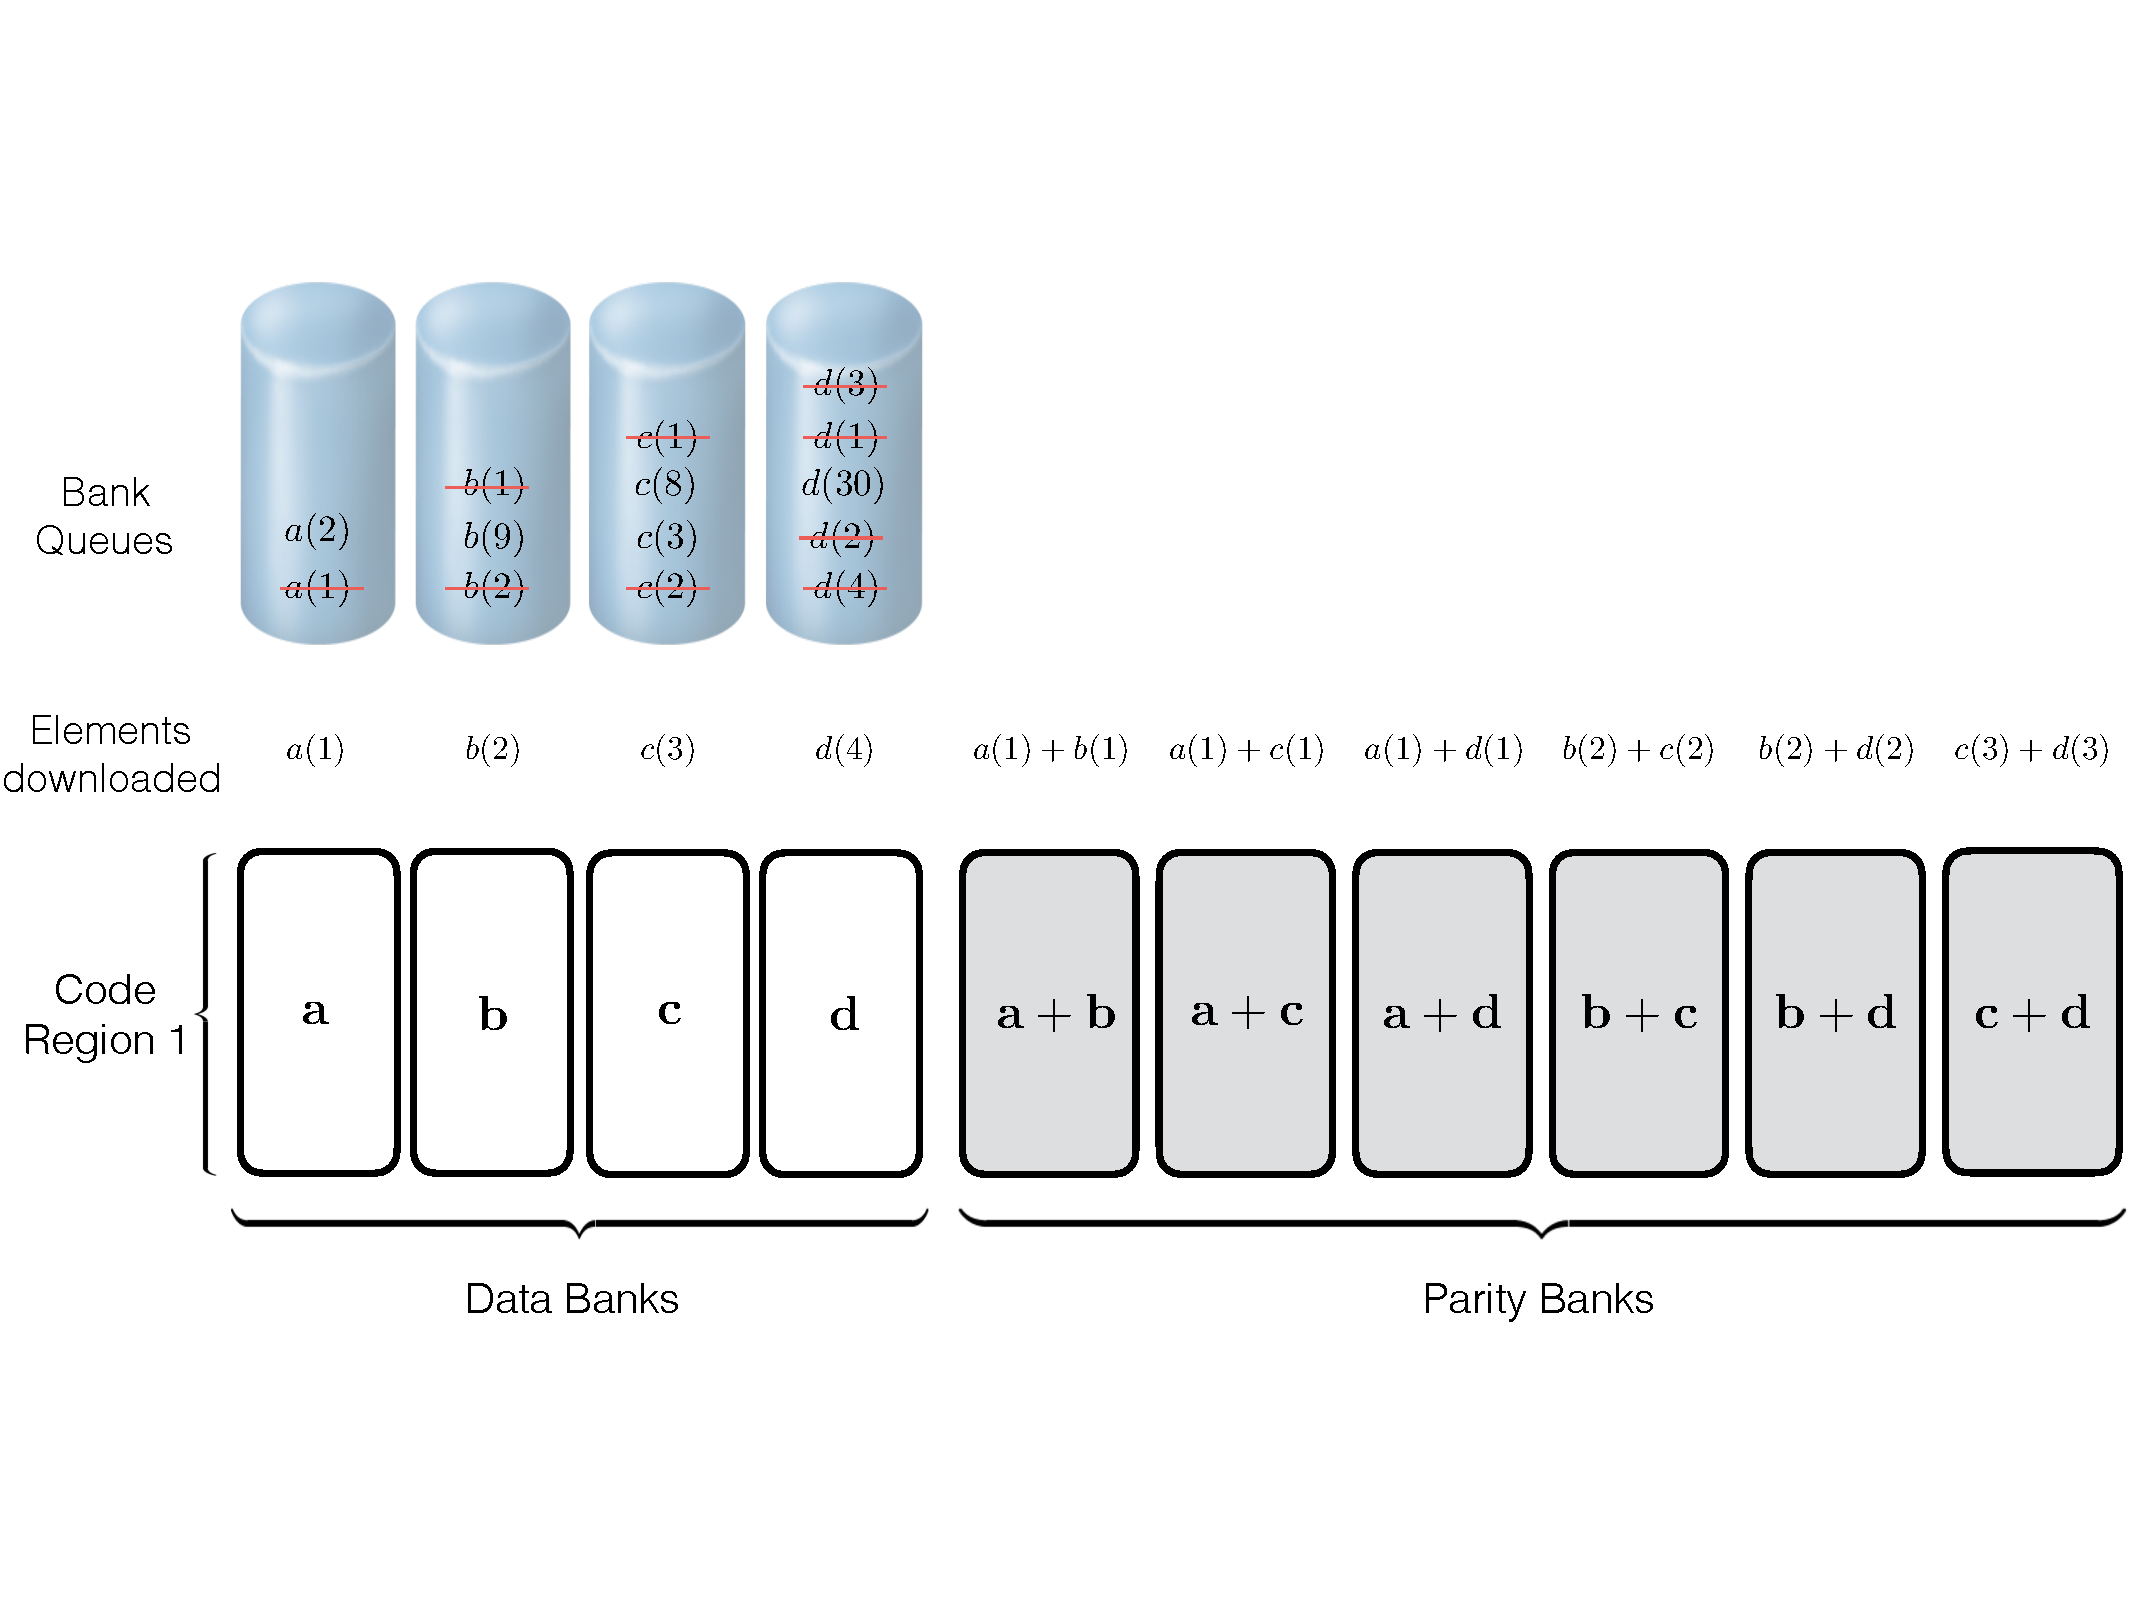
\includegraphics[width=0.96\linewidth]{fig/Read-Algo-Example.pdf}
	\caption{{Illustration of the algorithm to build a read request pattern to be served in a given memory cycle. All the read requests associated with the strikethrough elements are scheduled to be served in a given memory cycle. The figure also shows the elements downloaded from all the memory banks in order to serve these read requests.}}
	\label{fig:readAlgoAccessPattern}
\end{figure}
%------------------------
%\subsection{Read Algorithm for Coded Memory system}
\subsection{Read pattern builder}
\label{sec:readCodingAlgo}


The access scheduler uses the read pattern builder algorithm to determine which requests to serve using parity and which to use data banks. The read pattern builder selects which memory requests to serve and determines how requests served by parity banks will be decoded. The algorithm is designed to serve many read requests in a single memory cycle. Figure~\ref{fig:readAlgo} shows our implementation of the read pattern builder.

Figure~\ref{fig:readAlgoAccessPattern} shows an example read pattern constructed by our algorithm. First, $a(1)$ is marked to be read from data bank $\mathbf{a}$. Then the algorithm looks through banks $\mathbf{b}$, $\mathbf{c}$, and $\mathbf{d}$ for requests for rows $b(1)$, $c(1)$, or $d(1)$ because these symbols can be decoded from a parity bank using the $a(1)$ symbol. In this scenario all three are present in the bank queues and are served using parity banks. Symbols equal to  $a(1) + b(1)$, $a(1) + c(1)$, and $a(1) + d(1)$ are all downloaded from parity banks and decoded with $a(1)$. Next, $b(2$) is read from a data bank. Similar to before, $c(2)$ and $d(2)$ are served by downloading $b(2) + c(2)$ and $b(2) + d(2)$ symbols from the parity banks. Again as before, $c(3)$ is read from data bank and $d(3)$ is decoded using $c(3)$ and $c(3) + d(3)$. Finally, $d(4)$ is read from a data bank.

\begin{remark}
By increasing the number of read requests per cycle, we increase the risk of having out-of-order execution of memory access requests on the same core. We assume that the code arbiter only admits requests into the bank queues if they can be immediately served without introducing harmful out-of-order execution.


\end{remark}
\ignore{
%-----------------------
\begin{figure}[htbp]
\centering
	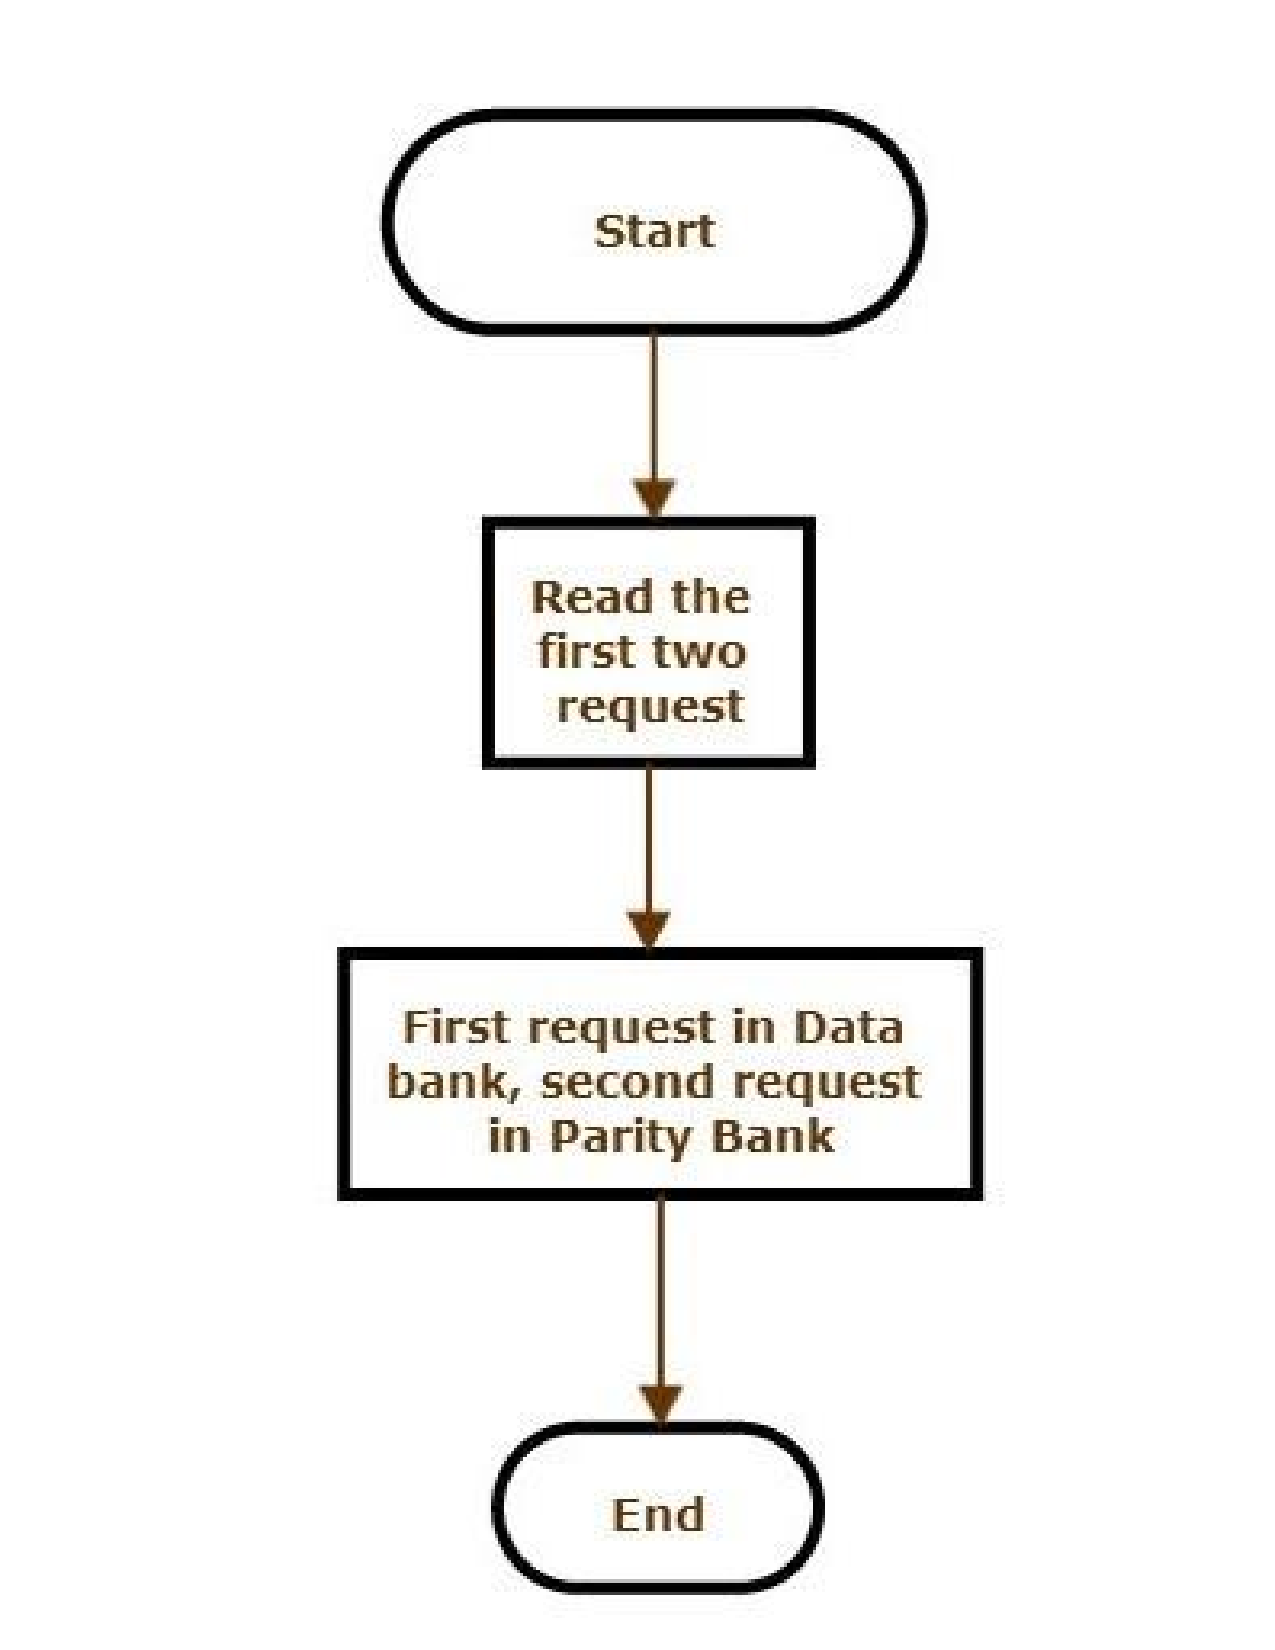
\includegraphics[width=\linewidth]{fig/writealgo.pdf}
	\caption{{\bf Flowchart of Write Algorithm}}
	\label{fig:writeAlgo}
\end{figure}
%-------------------------
%\ignore{
\begin{itemize}
\item Write about how we solve the out of order look ahead problem. If we solve 
	it at all ????
\end{itemize}
}
%\subsection{Write Algorithm for Coded Memory system}
\subsection{Write pattern builder}
\label{sec:writeCodingAlgo}
Parity banks allow the memory controller to serve additional write requests per cycle. When multiple writes target a single bank, it can commit some of them to parity banks. The access scheduler implements a write pattern builder algorithm to determine which write requests to schedule in a single memory cycle. Figure~\ref{fig:writeFlow} illustrates our implementation of the write pattern builder. Only when the write bank queues are nearly full does the access scheduler execute the write pattern builder algorithm. 


%-----------------------
\begin{figure}[htbp]
\centering
	\includegraphics[width=\linewidth]{fig/write_pattern_algo.png}
	\caption{{ Flowchart of write pattern builder}}
	\label{fig:writeFlow}
\end{figure}
%-------------------------


Figure~\ref{fig:writeAlgoAccessPattern} shows an example write pattern produced by our algorithm. Parity banks increase the maximum number of write requests from $4$ to $10$. Note that an element which is addressed to row $n$ in a data bank can only be written to the corresponding row $n$ in the parity banks. In this scenario, the write queues for every data bank are full. The controller takes $2$ write requests from each queue and schedules one to the queue's target data bank and the other to a parity bank. The controller also updates the code status table.

{\color{red}
Figure~\ref{fig:writeAlgoAccessPattern} also demonstrates how the code status table changes to reflect the freshness of the elements in the data and parity banks. Here, the 00 status indicates that all elements are updated. The 01 status indicates that the data banks contain fresh elements and the elements in the parity banks must be recoded. The 10 status indicates that the parity banks contain fresh elements, and that both data banks and parity banks must be updated.
}

%-----------------------
\begin{figure}[t!]
\centering
         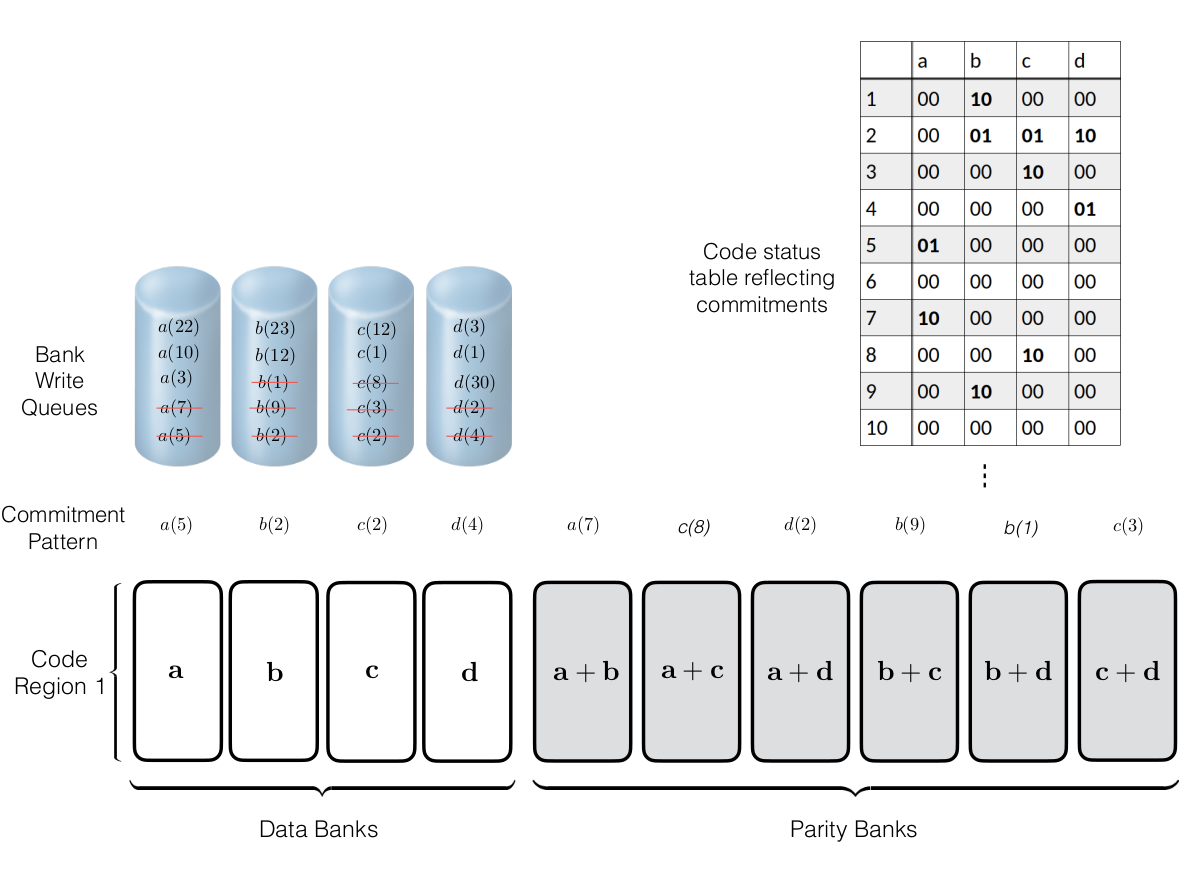
\includegraphics[width=\linewidth]{fig/Write-Algo-Example.png}
	\caption{The behavior of the write pattern builder on a 4-bank memory system}
	\label{fig:writeAlgoAccessPattern}
\end{figure}
%-------------------------
\subsection{ReCoding unit}
\label{sec:recoding}
After a write request has been served, the stale data in the parity (or data) banks must be replaced. The \textit{ReCoding Unit} accomplishes this with a queue of {\em recoding requests}. Every time a write is served, recoding requests are pushed on to the queue indicating which data and parity banks contain stale elements, as well as the bank which generated the recoding request. Requests also contain the current cycle number so that the ReCoding Unit may prioritize older requests. Appendix

\subsection{Dynamic Coding}
\label{sec:dynamicCoding}
To reduce memory overhead $\alpha$, parity banks are designed to be smaller than data banks. The dynamic coding block maintains codes for the most heavily accessed memory subregions, so that parity banks are utilized more often.
%
%\subsubsection{Encoder Design}
%There are many possible implementations of the dynamic coding unit. The design described here is used in the simulator used to generate the results described in sections 5 and 6.
%
The {\em dynamic coding} block partitions each memory bank into $\lceil\frac{1}{r}\rceil$ regions. The block can select up to $\frac{\alpha}{r} - 1$ regions to be encoded in the parity banks. A single region is reserved to allow encoding of a new region.

Every $T$ cycles, the dynamic coding unit chooses the $\frac{\alpha}{r} - 1$ regions with the greatest number of memory accesses. The dynamic coding unit will then encode these regions in the parity banks. If all the selected regions are already encoded, the unit does nothing. Otherwise, the unit begins encoding the most accessed region. Once the dynamic coding unit is finished encoding a new region, the region becomes available for use by the rest of the memory controller. A memory region of length $r$ is reserved by the dynamic coding unit for constructing new encoded regions, and a memory region of length $\alpha - r$ is reserved for active encoded regions. If the memory ceiling $\alpha - r$ is reached when a new memory region is encoded, the unit evicts the least frequently used encoded region.

\subsection{Prefetching Codes}
\label{sec:prefetching}
Dynamic coding works best when the most heavily accessed regions of memory vary little to none over time. When the memory access trend is not static, the proposed memory system can benefit from anticipating structured (\textit{e.g.} sequential) memory accesses. Therefore, our design includes a prefetcher which detects sequential memory accesses and exploits idle memory banks to potentially serve future memory requests. The prefetcher prioritizes long sequential memory accesses as motivation for performing an anticipatory read. Because of the speculative nature of the prefetcher, it is given the lowest priority of all the components in the access scheduler. It only schedules a memory access if all the other units have not done so first. 
\Ethan{More details here?}

%%%%%%%%%%%%%%%%%%%%%%%%%%%%%%%%%%%%%%%%%%%%%%%%%%%%%%%%
% Experimental Methodology
%%%%%%%%%%%%%%%%%%%%%%%%%%%%%%%%%%%%%%%%%%%%
\section{Experimental Methodology}
\label{sec:experimentalmethodology}

In this section, we discuss our method for evaluating the performance of the proposed memory systems. We utilize the PARSEC v2.1 and v3.0 benchmark suites with the gem5 simulator to generate memory traces. Next, we run the Ramulator DRAM simulator to to measure the performance of the proposed memory systems. We compare the baseline performance of the Ramulator simulators against a modified version of the Ramulator simulator which implements the proposed memory systems.

\subsection{Memory Trace Generation}

We use the PARSEC benchmark suite to evaluate the performance of the proposed memory systems. The PARSEC benchmark suite was developed for Chip Multiprocessors and is composed of a diverse set of multithreaded applications~\cite{bienia09parsec2}. The benchmarks allow us to observe how the proposed memory systems perform in dense memory access scenarios. A number of input sets are provided alongside the PARSEC benchmarks. To run the PARSEC applications, we use the gem5 simulator~\cite{parsec_2_1_m5}.

The gem5 simulator allows us to select the number of processors and their attributes we use to generate the memory traces. For most traces, we used 8 processors for the PARSEC benchmarks we evaluated. We also used 16 and 32 processors to explore the effects of denser memory traces on the Ramulator simulation results. The PARSEC applications can be divided into multiple regions where the nature of the computation therein differs. The most computationally interesting region is the region where parallel processing takes place. We extract the region of the trace where the application was performing parallel processing, as it is this region where there is a high probability for bank conflicts to occur. Thus, our Ramulator simulations are run only on this parallel portion of the PARSEC benchmarks.

\Matt{TODO: List the input sets used for each benchmark(?)}

We convert the gem5 memory traces to the Ramulator CPU-trace format. The conversion process is simple as it only requires the reorganization of the memory addresses in the gem5 memory trace. It is important that we use the Ramulator CPU-trace format and not the DRAM-trace format because the CPU-trace format contains information necessary to simulate the processor subsystem within Ramulator, the subsystem wherein the memory controller lies.

\subsection{PARSEC Trace Attributes}

The most important attributes of the memory traces as it relates to the proposed memory systems is the density of the traces, the overlap of the memory accesses between the processors, and how stationary the heavily utilized regions of memory are. The PARSEC benchmarks are sufficiently dense as illustrated by Figure~\ref{fig:dedup_dense}. It is clear from this image that there is heavily memory utilization during this section of the Dedup benchmark. On average across all processors, there is an average of 1.11 nanoseconds between memory accesses per core. The equates to an average of 2.22 cycles between memory access requests per 2 Ghz processor. 

The location of the most heavily used memory region is stationary with respect to time for all PARSEC benchmarks. Figure~\ref{fig:dedup_whole} shows the whole of a dedup memory trace. There are two major bands clear from this image, and the bands remain horizontal for the entirety of the plot indicating that these bands remain heavily accesses for duration of the trace. Figure~\ref{fig:dedup_dense} is a magnified view of the bottom band. This figure reveals that the bottom band is composed of two sub-bands which are also stationary with respect to time. The structure of the dedup the memory trace is representative for all the PARSEC benchmarks. It is also clear from this image that the memory regions utilized by all of the processors overlap sufficiently to create bank conflicts.

\subsection{Ramulator}

We use the Ramulator DRAM simulator to compare the number of CPU cycles required to execute the PARSEC memory traces. We use the vanilla Ramulator simulator to acquire the baseline number of CPU cycles. We extended the memory controller in Ramulator in order to simulate the proposed memory system, and we use the modified Ramulator to examine the improvements the memory system has over the baseline. We use a consistent Ramulator configuration file so that the improvements we observe over baseline are purely a result of the memory system resolving bank conflicts. We test across the amount of memory overhead $\alpha$ the memory system is permitted to use. 
The following are the specifics of the Ramulator configuration file used to acquire the simulation results:
\begin{itemize}
\item Standard : HBM
\item Channels: 8
\item Ranks: 1
\item Speed: 1 Gigabits per second
\item Organization: 4 Gigabits
\item CPU ticks: 32
\item Memory ticks: 5
\end{itemize}



%%%%%%%%%%%%%%%%%%%%%%%%%%%%%%%%%%%%%%%%%%%%%%%%%%%%%%%%
% Results
%%%%%%%%%%%%%%%%%%%%%%%%%%%%%%%%%%%%%%%%%%%%
\subsection{Simulation Results}
\label{sec:simulation}
%\Matt{BLUE: I would not mind removing this text. RED: I will likely remove this text}
%The simulation results are consistent across all the PARSEC benchmarks. The reason for this consistency is due to the similarity of the memory traces across the benchmarks. 

Given sufficient memory overhead, we see a consistent 25\% reduction in CPU cycles over the baseline simulation, with Coding Scheme I generally performing best. 

%\subsection{PARSEC Results}

The proposed memory system performs consistently across the PARSEC benchmarks, and the three proposed schemes yield similar results. Figure~\ref{fig:dedup_results} shows the simulation results for the dedup benchmark with a memory partition coefficient $r = 0.05$. The plot shows that the number of CPU cycles is reduced by $73\%--83\%$ once sufficient memory overhead $\alpha$ is used. 
%The lines on this figure and others show the number of CPU cycles needed for the Ramulator simulation to finish executing. 
We also see that the number of memory region switches performed by the dynamic encoder. When $\alpha = 1$, the number of switches is always zero as expected because the dynamic encoder never needs to switch regions. The performance remains consistent for $\alpha > 0.1$. With this amount of overhead, the memory system finds and encodes the two heavily accessed memory bands in each of the PARSEC benchmarks. This is because $\lfloor\frac{\alpha}{r}\rfloor = 2$, which means we can select $2$ regions to encode. 
%The number of coded region switches is evidence that at $\alpha = .05$ more memory is needed to see maximum benefits from the memory system. 
When $\alpha = 0.05$, the number of coded region switches is very high because the memory system vacillates between the two most heavily accessed bands. When $\alpha = .1$, both of them can be encoded. We see a small numbers of switches when $\alpha \geq 0.25$ because the memory system is encoding less heavily accesses memory bands with little impact on number of CPU cycles.


The heavily accessed memory bands are narrow, which suggests that decreasing the memory bank partition will result in similar performance improvements with a lower $\alpha$. Figure~\ref{fig:dedup_hundreth} shows that indeed $\alpha$ can be reduced by a factor of $5$ by also decreasing $r$ from $0.05$ to $0.01$.


%\subsection{PARSEC Augmentation}
%\subsection{Augmentation}

\subsubsection{Augmented PARSEC}

Results on the the augmented PARSEC traces show that our system improves over the baseline to a lesser extent.
%
%results significantly impact the Ramulator simulation results. Increasing the number of memory bands by splitting the dense bands results in an increased memory requirement to see improved performance. Introducing a ramp to the memory bands decreases the efficacy of the proposed memory system across all values of $\alpha$. \Ethan{highlight it's still good}
%
Figure~\ref{fig:vips_split_result} shows that for a large number of memory bands, we can achieve the same performance as before only by increasing the memory overhead or increasing the memory partition coefficient.
% The memory partition coefficient used here is $r = .05$, but as shown in Figures ~\ref{fig:dedup_results} and ~\ref{fig:dedup_hundreth} lowering the memory partition coefficient allows a lowering of $\alpha$ while achieving the same performance.

Figure~\ref{fig:vips_ramp_result} shows the results of the ramp augmentation. Here we see that our system struggles to adapt to a constantly changing primary access region. 

%The proposed memory system performace worse in this scenario. The number of memory region switches shows that the memory system struggles to handle the constantly changing location of the heavily accessed memory regions. 

%The reason for this is that the memory system locates the heavily accessed memory regions and rarely switches away from them. Here, the memory system is constantly attempting to catch up with the heavily accessed memory region. {\color{blue}We note that the ramp covers a very large number of memory addresses, so the decrease in performance we observe would only effect programs which use very large portions of memory.} 

\begin{figure}[htbp]
		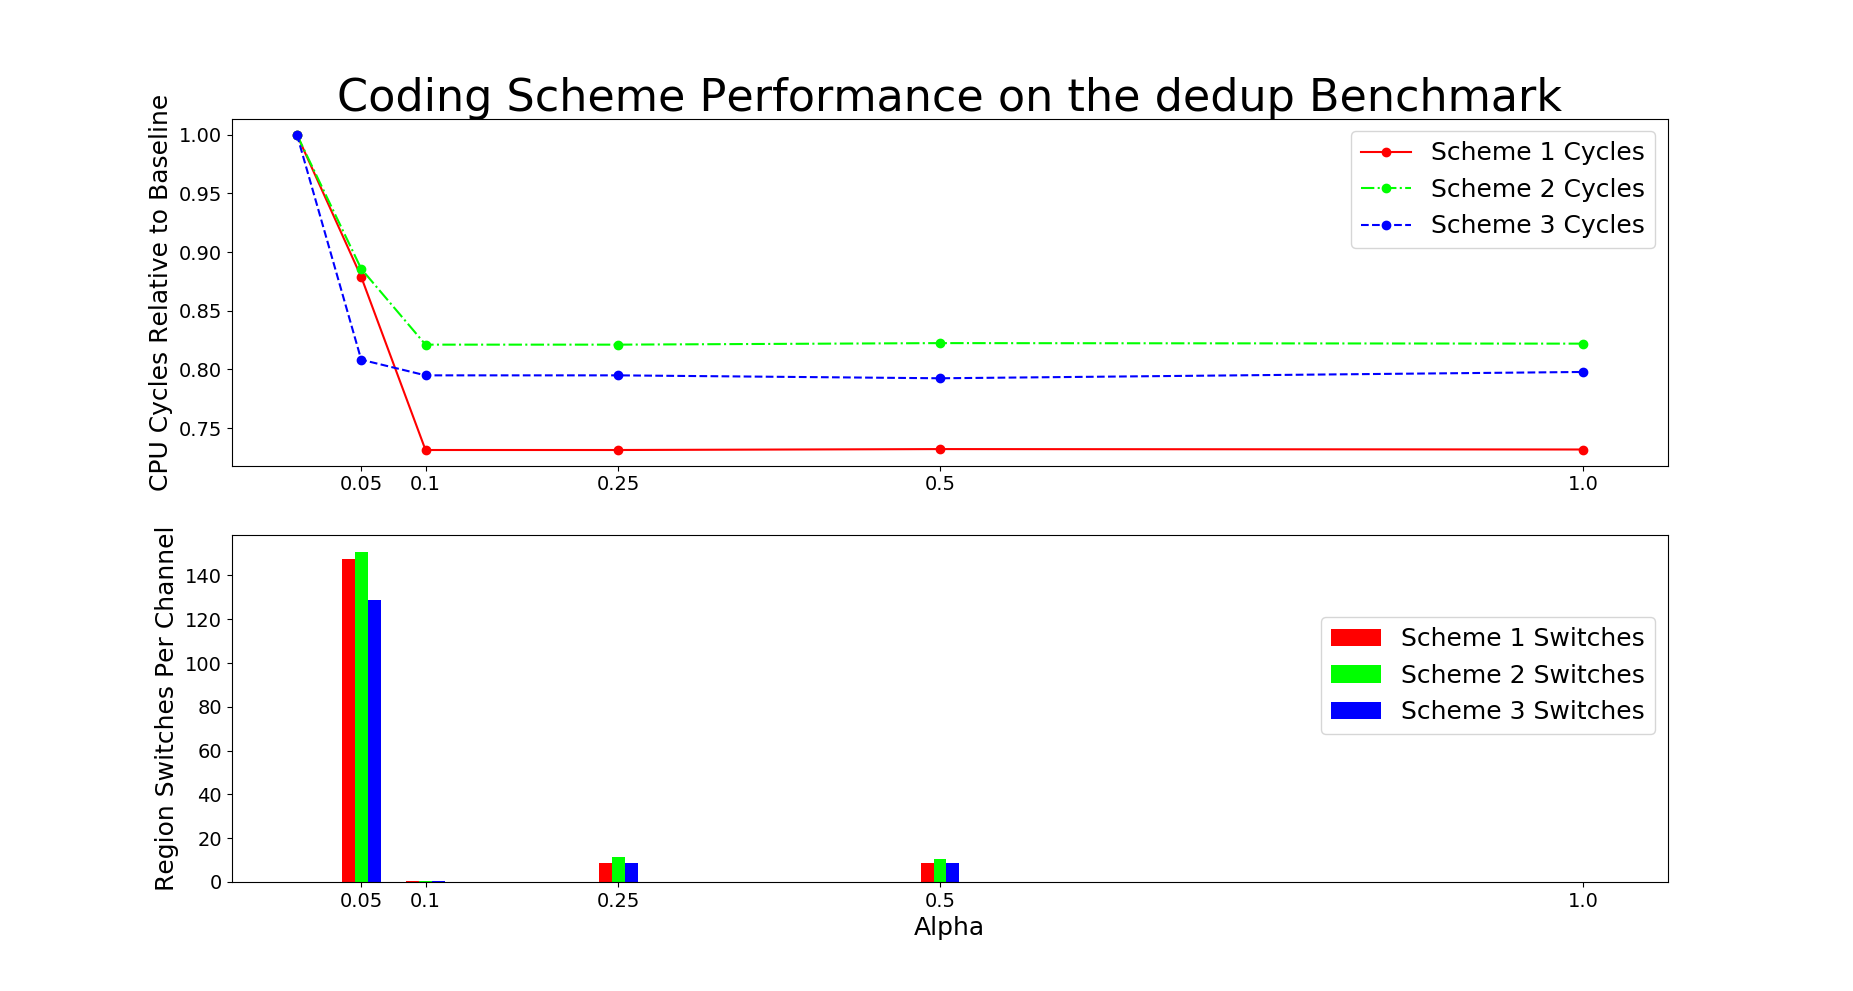
\includegraphics[width=\linewidth]{fig/dedup_benchmark_results.png}
		\caption{The simulation results for the dedup PARSEC benchmark. The line plot represents the number of CPU cycles needed and the bar plot represents the number of items the dynamic coding unit chooses to encode a new memory region. The results from the other PARSEC benchmarks are similar.}
		\label{fig:dedup_results}
\end{figure}

\begin{figure}[htbp]
		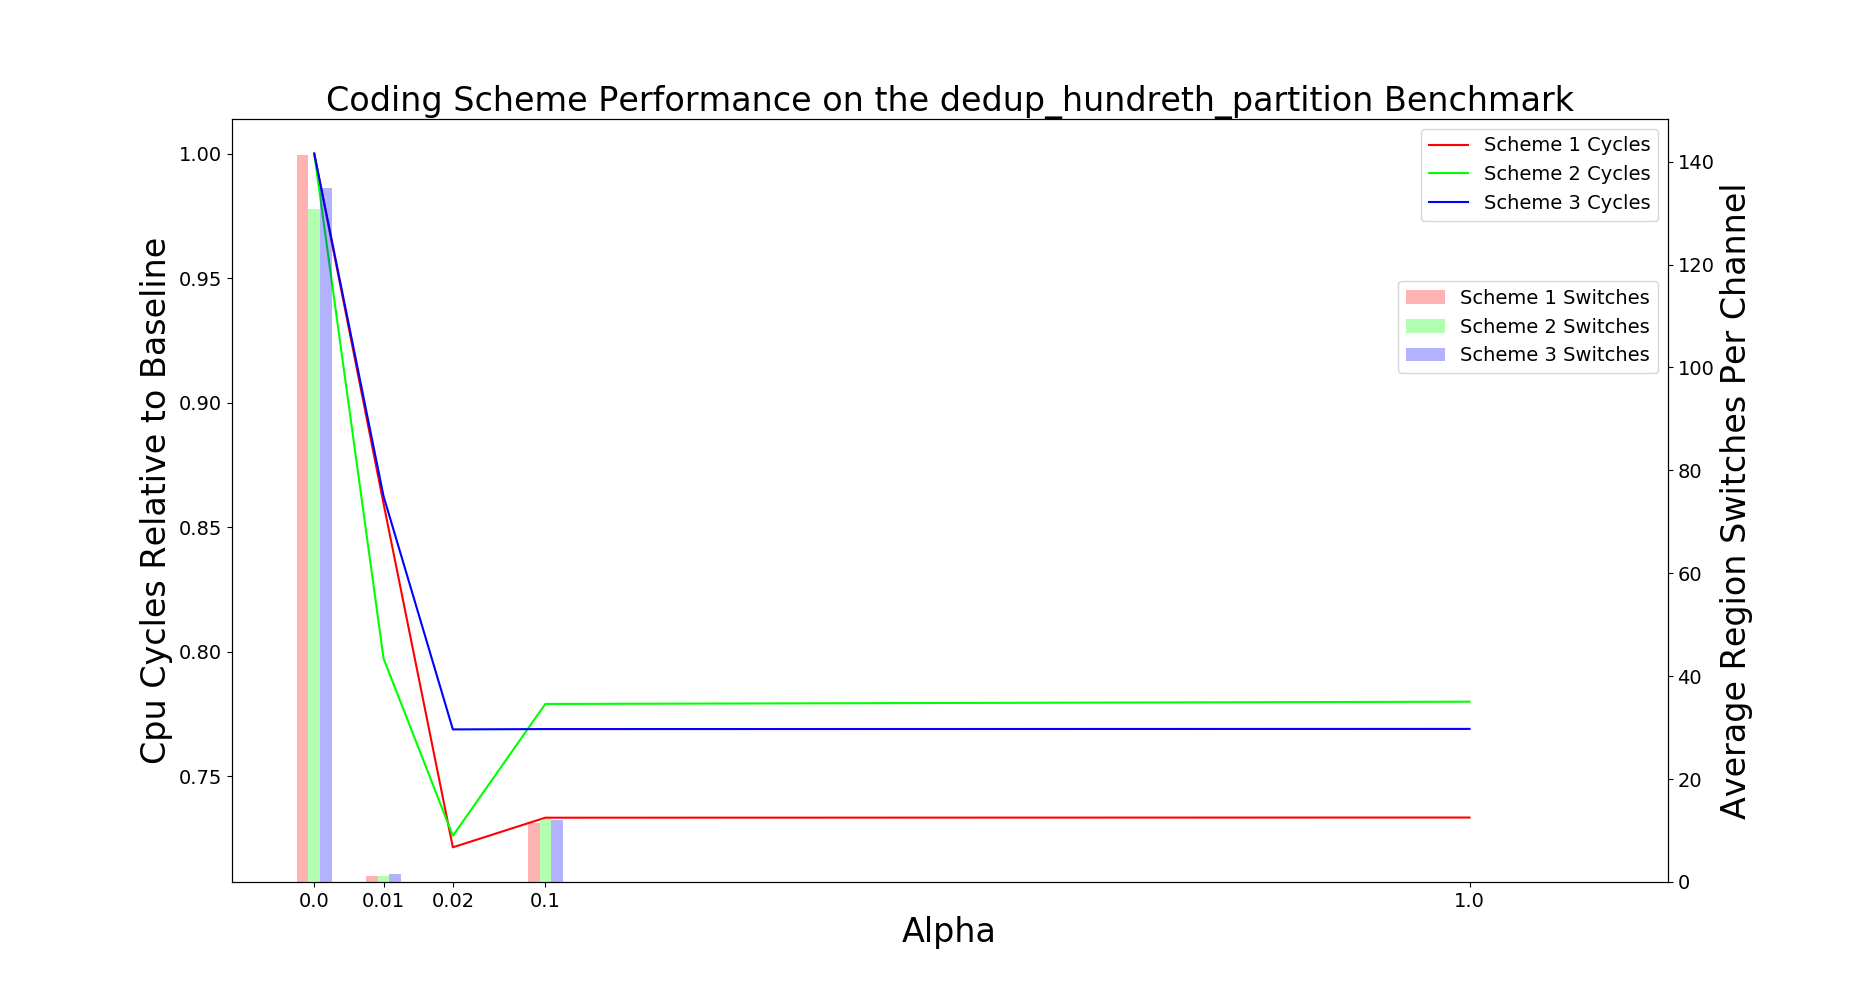
\includegraphics[width=\linewidth]{fig/dedup_hundreth.png}
		\caption{The simulation results for the same trace simulated in Figure~\ref{fig:dedup_results} but with a memory partition coefficient $r = .01$}
		\label{fig:dedup_hundreth}
\end{figure}

\begin{figure}[htbp]
		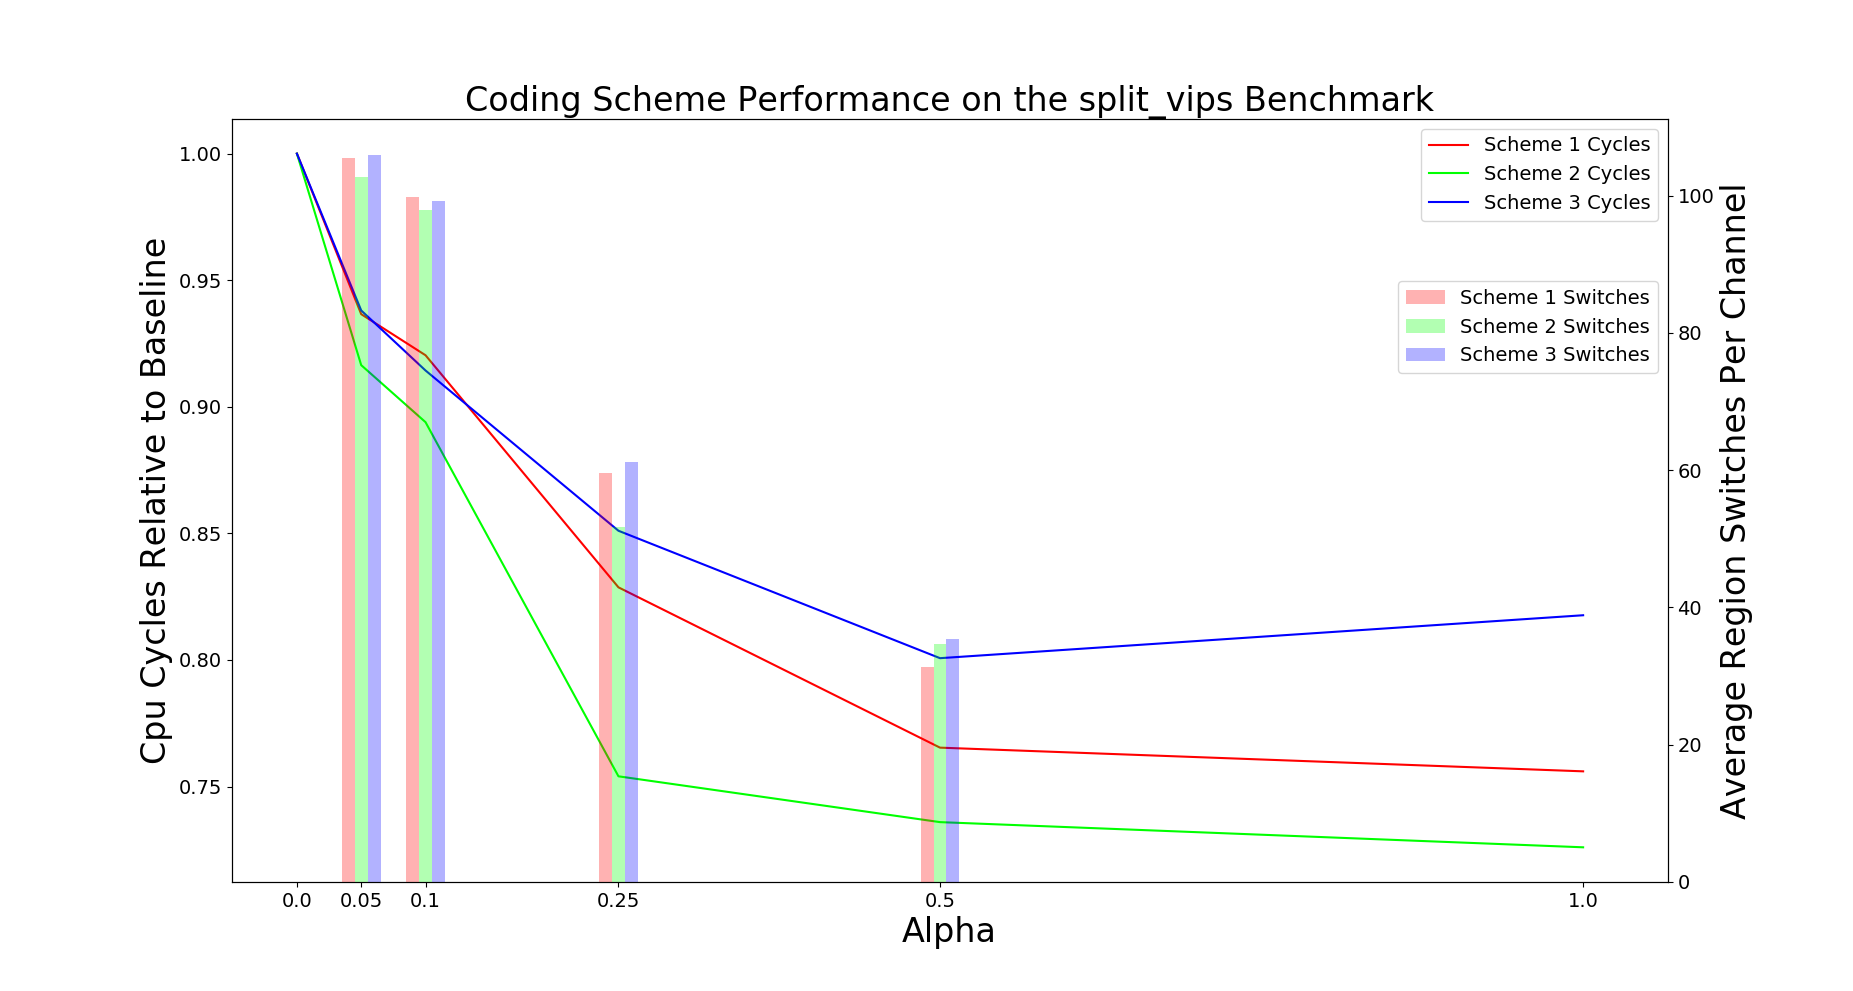
\includegraphics[width=\linewidth]{fig/vips_split_results.png}
		\caption{The simulation results of the augmented vips trace pictured in Figure~\ref{fig:vips_split}}
		\label{fig:vips_split_result}
\end{figure}

\begin{figure}[htbp]
		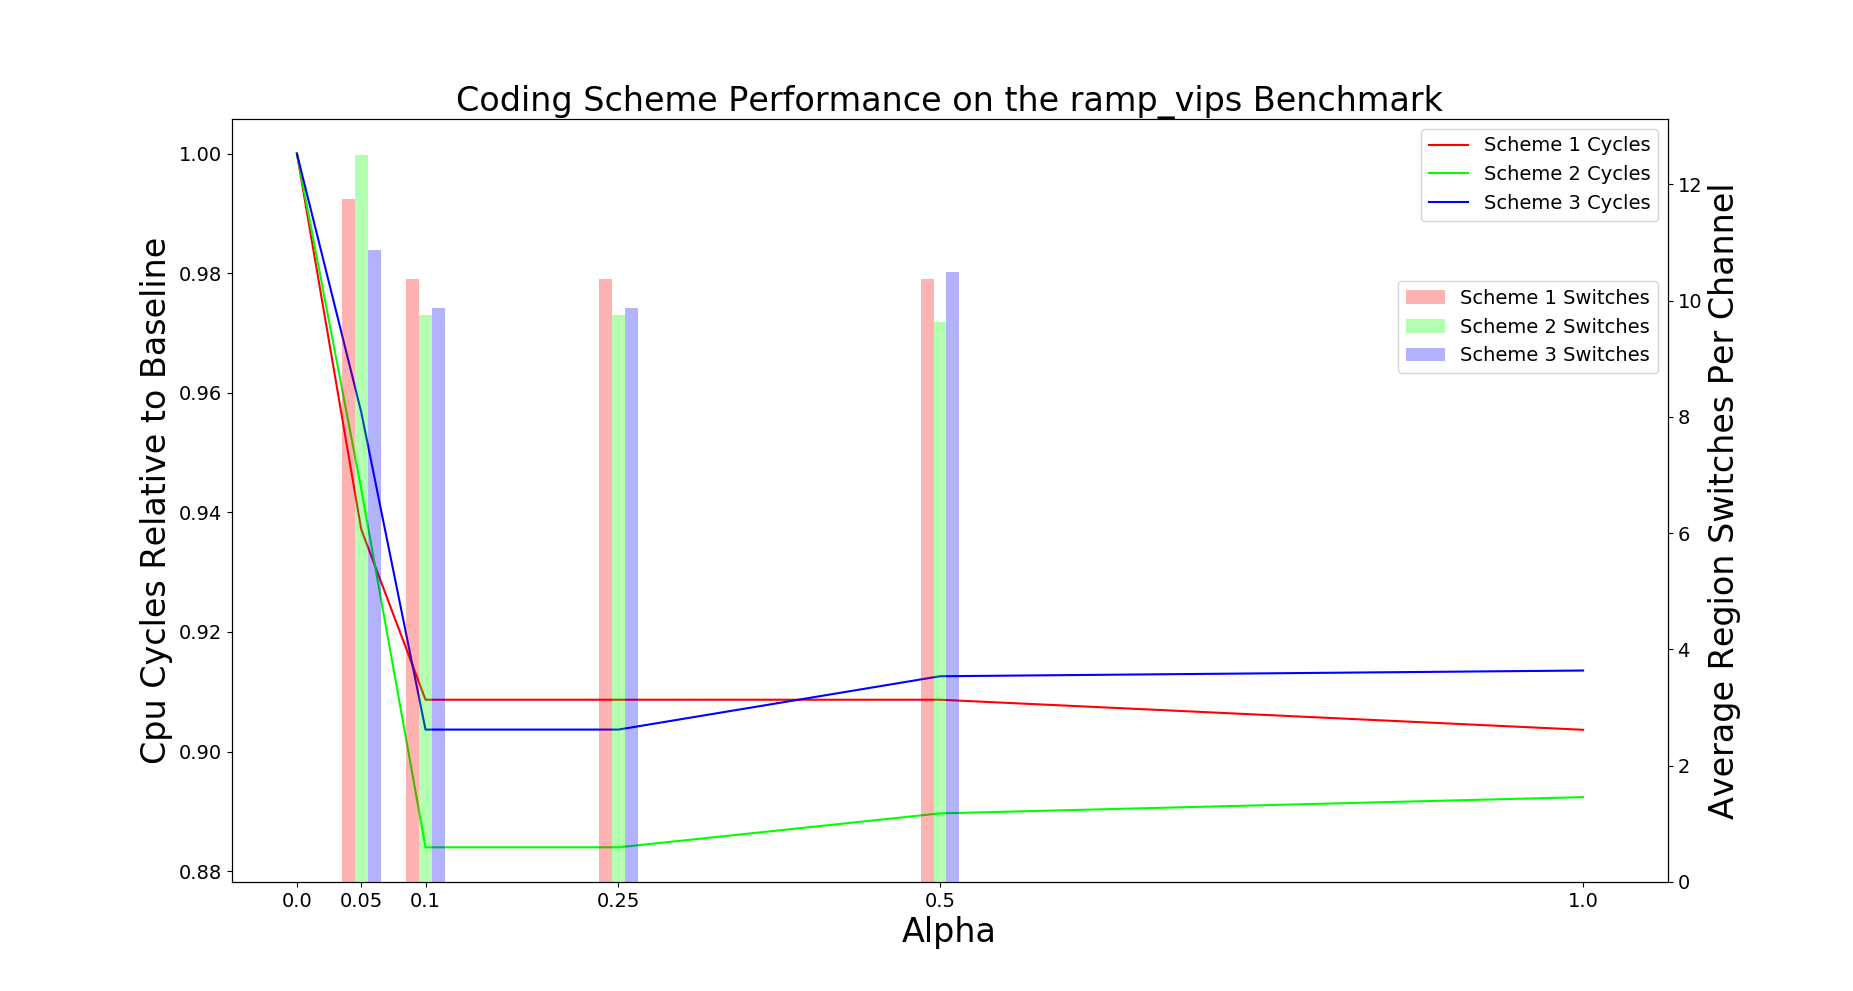
\includegraphics[width=\linewidth]{fig/vips_ramp_results.png}
		\caption{The simulation results of the augmented vips trace pictured in Figure~\ref{fig:vips_ramp}}
		\label{fig:vips_ramp_result}
\end{figure}




%%%%%%%%%%%%%%%%%%%%%%%%%%%%%%%%%%%%%%%%%%%%%%%%%%%%%%%%
% Conclusion
%%%%%%%%%%%%%%%%%%%%%%%%%%%%%%%%%%%%%%%%%%%%


%%%%%%%%%%%%%%%%%%%%%%%%%%%%%%%%%%%%%%%%%%%%%%
% Acknowledgements
%%%%%%%%%%%%%%%%%%%%%%%%%%

\section{Acknowledgements}
This document is derived from previous conferences, in particular HPCA 2017.  We thank Daniel A. Jimenez,  Elvira Teran for their inputs.



%{\color{red}\textbf{Coding over small number of banks:~}In order to save storage space allocated to different pointers.....This is something which does not arise in many classical scenarios where coding is employed. For example, in communications, it is preferable to encode over long messages as apart from computational complexity as in most cases there is no additional penalty (proportional to the code length) in terms of pointers required to deal with write requests.}

%In this part, we attempt to design efficient codes based on the memory traces 
%shared by Huawei.  The goal of this design was to simulate the efficiency of 
%coding and compare the results to the baseline implementation of not coding.  
%During this design phase, we explored various code functions that could be used 
%to create the codes on the stored data. We decide upon using the XOR function to 
%store the data in the parity banks because of its low complexity overhead and 
%for preserving the linearity of codes. Linear codes offer the widest range of 
%functionality because any order of the codes may be used to either encode or 
%decode. This lack of dependency allows our design to use the parity banks in the 
%most flexible way possible. We also explore the potential benefits of using 
%different weights to the memory elements for the XOR function. For examples, the 
%memory elements $a_0$ and $b_0$ could be stored as $\alpha a_0 + \beta b_0$ for 
%integer values of $\alpha$ and $\beta$ which belong to any Galois Field. The 
%least complex design for the decoder would be for taking $\alpha$ = 1 and 
%$\beta$ = 1 . Another design consideration explored is the compression factor to 
%generate the codes.  The codes can be generated by using xor on 2 or more memory 
%elements. For example, suppose there are four banks A, B , C and D. Each of the 
%banks hold $a_0$ to $a_n$, $b_0$ to $b_n$ , $c_0$ to $c_n$ and $d_0$ to $d_n$ 
%elements respectively. The possible codes for these memories could be:
%\begin{equation}
%a_i + b_i, b_i + c_i, c_i + d_i \text{ and } c_i + a_i  \text{ for i = 0 to n }
%\end{equation}
%This scheme uses the combination of 2 memory elements to generate the codes.  
%Although this requires 100$\%$ extra memory overhead, it enables 100$\%$ extra 
%memory accesses per cycle, i.e., 4 extra accesses in this case.
%Another design could be to compress the codes by combining all 4 memory elements 
%to generate the codes:
%\begin{equation}
%a_i + b_i + c_i + d_i \text{ for i = 0 to n }
%\end{equation}
%This design gives one extra access per cycle at the cost of 25$\%$ memory 
%overhead. However, the decoder here needs to know 3 elements to be able to 
%decode the 4th element. So although we are able to compress more data into a 
%single memory location, it comes with the cost of additional memory logic.  The 
%scheme described above "codes" the memory banks using elements from different 
%banks. We call this type of coding as Interbank Coding. We also explore the 
%orthogonal way of coding, i.e. intra-bank coding where we use the memory 
%elements from the same bank to generate codes.
%\\
Following are the objectives used in code design:
\begin{itemize}
\item Read access : 4 per bank in one cycle
\item Write access : 2 per bank in one cycle
\item Shared Memory size 8 kB - 256 kB
\item Number of Banks : 8
\item Memory overhead : 15$ \% $
\item Parity banks : 5 or 6 shallow banks for code storage
\end{itemize}


%%%%%%% -- PAPER CONTENT ENDS -- %%%%%%%%

\newpage

%%%%%%%%% -- BIB STYLE AND FILE -- %%%%%%%%
%\bibliographystyle{ieeetr}
\bibliographystyle{IEEEtran}
\bibliography{references}
%%%%%%%%%%%%%%%%%%%%%%%%%%%%%%%%%%%%

\end{document}
